%% ******************************* PhD Thesis Template **************************
% Please have a look at the README.md file for info on how to use the template

\documentclass[a4paper,12pt,times,numbered,print,index,custommargin]{Classes/PhDThesisPSnPDF}

\usepackage{nomencl, tikz} 
\def\checkmark{\tikz\fill[scale=0.4](0,.35) -- (.25,0) -- (1,.7) -- (.25,.15) -- cycle;}

\makenomenclature


% `a4paper'(The Politecnico di Torino PhD thesis guidelines recommends a page
% size a4 - default option) or `a5paper'%
% `11pt' or `12pt'(default): Font Size 10pt is NOT recommended by the University
% guidelines
% `oneside' or `twoside'(default): Printing double side (twoside) or single
% side.
% `print': Use `print' for print version with appropriate margins and page
% layout. Leaving the options field blank will activate Online version.

% `abstract': To generate only the title page and abstract page with
% dissertation title and name, to submit to the Student Registry
%
% `chapter`: This option enables only the specified chapter and it's references
%  Useful for review and corrections.
%
% ************************* Custom Page Margins ********************************
%
% custommargin`: Use `custommargin' in options to activate custom page margins,
% which can be defined in the preamble.tex. Custom margin will override
% print/online margin setup.
%
% *********************** Choosing the Fonts in Class Options ******************
%
% `times' : Times font with math support. (The Polito guidelines
% recommend using times)
%
% `fourier': Utopia Font with Fourier Math font (Font has to be installed)
%            It's a free font.
%
% `customfont': Use `customfont' option in the document class and load the
% package in the preamble.tex
%
% default or leave empty: `Latin Modern' font will be loaded.
%
% ********************** Choosing the Bibliography style ***********************
%
% `authoryear': For author-year citation eg., Rossi (2013)
%
% `numbered': (Default Option) For numbered and sorted citation e.g., [1,5,2]
%
% `custombib': Define your own bibliography style in the `preamble.tex' file.
%              `\RequirePackage[square, sort, numbers, authoryear]{natbib}'.
%              This can be also used to load biblatex instead of natbib
%              (See Preamble)
%
% **************************** Choosing the Page Style *************************
%
% `default (leave empty)': For Page Numbers in Header (Left Even, Right Odd) and
% Chapter Name in Header (Right Even) and Section Name (Left Odd). Blank Footer.
%
% `PageStyleI': Chapter Name next & Page Number on Even Side (Left Even).
% Section Name & Page Number in Header on Odd Side (Right Odd). Footer is empty.
%
% `PageStyleII': Chapter Name on Even Side (Left Even) in Header. Section Number
% and Section Name in Header on Odd Side (Right Odd). Page numbering in footer


% ********************************** Preamble **********************************
% Preamble: Contains packages and user-defined commands and settings
% ******************************************************************************
% ****************************** Custom Margin *********************************

%Add `custommargin' in the document class options to use this section
%Set {innerside margin / outerside margin / topmargin / bottom margin}  and
% other page dimensions
\ifsetCustomMargin
  \RequirePackage[left=25mm,right=25mm,top=40mm,bottom=40mm]{geometry}
  \setFancyHdr % To apply fancy header after geometry package is loaded
\fi

% Add spaces between paragraphs
\setlength{\parskip}{0.5em}
% Ragged bottom avoids extra whitespaces between paragraphs
\raggedbottom
% To remove the excess top spacing for enumeration, list and description
%\usepackage{enumitem}
%\setlist[enumerate,itemize,description]{topsep=0em}

% *****************************************************************************
% ******************* Fonts (like different typewriter fonts etc.)*************

% Add `customfont' in the document class option to use this section

\ifsetCustomFont
  % Set your custom font here and use `customfont' in options. Leave empty to
  % load computer modern font (default LaTeX font).
  %\RequirePackage{helvet}

  % For use with XeLaTeX
  %  \setmainfont[
  %    Path              = ./libertine/opentype/,
  %    Extension         = .otf,
  %    UprightFont = LinLibertine_R,
  %    BoldFont = LinLibertine_RZ, % Linux Libertine O Regular Semibold
  %    ItalicFont = LinLibertine_RI,
  %    BoldItalicFont = LinLibertine_RZI, % Linux Libertine O Regular Semibold Italic
  %  ]
  %  {libertine}
  %  % load font from system font
  %  \newfontfamily\libertinesystemfont{Linux Libertine O}
\fi

% *****************************************************************************
% **************************** Custom Packages ********************************

% ************************* Algorithms and Pseudocode **************************

%\usepackage{algpseudocode}


% ********************Captions and Hyperreferencing / URL **********************

% Captions: This makes captions of figures use a small font.
\RequirePackage[small]{caption}

\RequirePackage[labelsep=space,tableposition=top]{caption}
\renewcommand{\figurename}{Fig.} %to support older versions of captions.sty


% *************************** Graphics and figures *****************************

%\usepackage{rotating}
%\usepackage{wrapfig}

% Uncomment the following two lines to force Latex to place the figure.
% Use [H] when including graphics. Note 'H' instead of 'h'
\usepackage{float}
%\restylefloat{figure}

% Subcaption package is also available in the sty folder you can use that by
% uncommenting the following line
% This is for people stuck with older versions of texlive
%\usepackage{sty/caption/subcaption}
\usepackage{subcaption}

% ********************************** Tables ************************************
\usepackage{booktabs} % For professional looking tables
\usepackage{multirow}

%\usepackage{multicol}
%\usepackage{longtable}
%\usepackage{tabularx}


% *********************************** SI Units *********************************
\usepackage{siunitx} % use this package module for SI units


% ******************************* Line Spacing *********************************

% Choose linespacing as appropriate. Default is one-half line spacing as per the
% University guidelines

% \doublespacing
% \onehalfspacing
% \singlespacing


% ************************ Formatting / Footnote *******************************

% Don't break enumeration (etc.) across pages in an ugly manner (default 10000)
%\clubpenalty=500
%\widowpenalty=500

%\usepackage[perpage]{footmisc} %Range of footnote options


% *****************************************************************************
% *************************** Bibliography  and References ********************

%\usepackage{cleveref} %Referencing without need to explicitly state fig /table

% Add `custombib' in the document class option to use this section
\ifuseCustomBib
   \RequirePackage[square, sort, numbers, authoryear]{natbib} % CustomBib

% If you would like to use biblatex for your reference management, as opposed to the default `natbibpackage` pass the option `custombib` in the document class. Comment out the previous line to make sure you don't load the natbib package. Uncomment the following lines and specify the location of references.bib file

%\RequirePackage[backend=biber, style=numeric-comp, citestyle=numeric, sorting=nty, natbib=true]{biblatex}
%\bibliography{References/references} %Location of references.bib only for biblatex

\fi

% changes the default name `Bibliography` -> `References'
\renewcommand{\bibname}{References}


% ******************************************************************************
% ************************* User Defined Commands ******************************
% ******************************************************************************

% *********** To change the name of Table of Contents / LOF and LOT ************

\renewcommand{\contentsname}{Contents}
\renewcommand{\listfigurename}{List of Figures}
\renewcommand{\listtablename}{List of Tables}


% ********************** TOC depth and numbering depth *************************

\setcounter{secnumdepth}{2}
\setcounter{tocdepth}{2}



% ******************************* Nomenclature *********************************

% To change the name of the Nomenclature section, uncomment the following line
%\renewcommand{\nomname}{Symbols}
%\printnomenclature[space] %space can be set as 2em between symbol and description
%\printnomenclature[3em]

% ********************************* Appendix ***********************************

% The default value of both \appendixtocname and \appendixpagename is `Appendices'. These names can all be changed via:

%\renewcommand{\appendixtocname}{List of appendices}
%\renewcommand{\appendixname}{Appndx}


% ************************ Thesis Information & Meta-data **********************
% Thesis title and author information, refernce file for biblatex
% ************************ Thesis Information ***************************

%% Title of the Degree (for example: mechanical engineering, Architecture,...)
\degreetitle{Industrial and Management Engineering}

%% Cycle of the phd program
%\cycle{$29^{th}$}

%% The title of the thesis
\title{Change detection and identification in Simple Serial Lines}
%\texorpdfstring is used for PDF metadata. Usage:
%\texorpdfstring{LaTeX_Version}{PDF Version (non-latex)} eg.,
%\texorpdfstring{$sigma$}{sigma}

%% Subtitle (Optional)
\subtitle{A manufacturing application of Process Mining}

%% The full name of the author
\author{Edoardo Chiò}
\label{author}

%% Supervisor(s) 
%% for multiple supervisors, append each supervisor with the \\ command
\supervisor{Prof. A.Alfieri, Supervisor\\
	Ph.D. E.Pastore, Co-Supervisor}%\\
	%Prof. E.F. ,Co-Supervisor\\
	%Prof. G.H. ,Co-Supervisor}

%% Committee members and their role, seperate the role and university by ,
\committee{Prof. A.B. , Referee, University of...\\
	Prof. C.D, Referee, University of... \\
	Prof. E.F, University of... \\ 
	Prof. G.H, University of... \\ 
	Prof. I.J, University of...}


%% Submission date
% Default is set as {\the\year}. In the case you want to change it use the command:
%\degreedate{2014} 

%% Meta information
\subject{LaTeX} \keywords{{LaTeX} {PhD Thesis} {Engineering} {Politecnico di Torino}}


% ***************************** Abstract Separate ******************************
% To printout only the titlepage and the abstract with the PhD title and the
% author name for submission to the Student Registry, use the `abstract' option in
% the document class.

\ifdefineAbstract
 \pagestyle{empty}
 \includeonly{Declaration/declaration, Abstract/abstract}
\fi

% ***************************** Chapter Mode ***********************************
% The chapter mode allows user to only print particular chapters with references
% Title, Contents, Frontmatter are disabled by default
% Useful option to review a particular chapter or to send it to supervisior.
% To use choose `chapter' option in the document class:

%\ifdefineChapter
% \includeonly{Chapter3/chapter3}
%\fi
% Then you can select the desired chapter (here is 3) to print.

% ******************************** Front Matter ********************************
\begin{document}

\frontmatter

\maketitle

% ******************************* Thesis Declaration ***************************

\begin{declaration}

I hereby declare that, the contents and organization of this dissertation constitute my own original work and does not compromise in any way the rights of third parties, including those relating to the security of personal data.

% Author and date will be inserted automatically from thesis.tex \author \degreedate

\end{declaration}


% ******************************* Thesis Dedidcation ********************************

\begin{dedication} 

\textit{to my loving parents\\ \medskip thanks for your patience}
%\textit{I would like to dedicate this thesis to my loving parents}

\end{dedication}


% ************************** Thesis Acknowledgements **************************

\begin{acknowledgements}      
Esprimo la mia gratitudine non solo a coloro che mi hanno aiutato direttamente con la tesi, ma anche a tutte le persone che hanno segnato il mio percorso universitario.\\
Ringrazio la professoressa Alfieri, per avermi offerto di svolgere questa tesi: le opportunità influenzano il corso del destino\\
Ringrazio la dottoressa Erica Pastore, per tutto l'aiuto che mi ha gentilmente offerto, sia nella preparazione della tesi e del paper, sia per il tirocinio\\
Ringrazio Claudio Castiglione, per i preziosi consigli su come procedere nella tesi nei momenti di confusione\\
Ringrazio Simone Grandi, il mio tutor aziendale durante il tirocinio, che con la sua personalità aperta e creativa è riuscito a offrirmi un approccio stimolante al mondo del lavoro\\
Ringrazio Alberto, che mi ha aiutato con grande pazienza quando i miei limiti come programmatore diventavano un ostacolo nella prosecuzione della tesi\\
Ringrazio Gabriele, per avermi aiutato con la tesi della laurea triennale, un vecchio simpaticissimo amico che ha subito risposto all’appello\\
Ringrazio Federico, per le conversazioni avute davanti a caffè e liquori fatti in casa, per essere un amico fidato con cui condividere i propri pensieri\\
Grazie a Irina, Ambra e Benedetta, compagne nei corsi più difficili, per il tempo passato insieme lottando per superare gli ostacoli universitari\\
Grazie a Matteo, Amedeo, Francesco, Davide e Laura, compagni di avventure in altri mondi; grazie a Lorenzo, per il tempo trascorso insieme fra videogiochi e meme; grazie a Jon, Andrea e Giulia, e a tutti i ragazzi dell’aula studio, per le partite a briscola durante la pausa caffè e le birre del venerdì sera\\
Grazie ad Anna e Lorenzo, amici fin dal liceo, perché pur avendo intrapreso percorsi diversi non ci siamo mai allontanati\\
Grazie a Riccardo, Giovanni e Gianluca, per le ore passate a discutere insieme mentre svolgevamo i progetti della magistrale, senza mai tirarsi indietro anche quando il lavoro diventava pesante\\
Grazie a Federico, Luca e Cesare, per la loro amicizia non scalfita dal tempo\\
Grazie a Clara, per aver ascoltato i miei sogni\\
Ringrazio Teodoro e Lucilla, perché le loro fusa mi hanno dato serenità nei momenti di ansia\\
Ringrazio Federica, la mia ragazza: se sono riuscito a concludere è grazie a lei, che mi ha incoraggiato senza incalzarmi, riuscendo a diffondere la luce dell’ottimismo nei tratti bui del mio percorso\\
Infine, più di tutti, ringrazio mio padre Adriano e mia madre Valeria, per il loro amore e supporto, offerti anche e soprattutto nei momenti più difficili; perché, come le guide migliori, indicano la strada giusta senza mai imporla; perché sono modelli di vita che incarnano le virtù della saggezza e dell’equilibrio come nessun altro.

\end{acknowledgements}

% ************************** Thesis Abstract *****************************
% Use `abstract' as an option in the document class to print only the titlepage and the abstract.
% The maximum number of characters in abstract must be 4000 (defined by PhD school of Politecnico di Torino). 
\begin{abstract}
According to the Industry 4.0 paradigm, Digital Twins of production systems must be always aligned with the real systems to guarantee an effective decision making process in a continuously changing environment. To keep the alignment, digital process models can be updated with Process Mining techniques through data collected by sensors. This thesis proposes a model-update procedure and addresses the issue of detecting and identifying changes occurring in Simple Serial Lines, a particular type of production lines. Using event logs, which are data structures generated by line embedded sensors, KPIs are computed, plotted, and analyzed to get insights of the system behavior. Simulation is used to test the effectiveness of the procedure.

\textit{Keywords}: manufacturing; Industry 4.0; digital twin; production systems; change identification; process mining.
\end{abstract}


% *********************** Adding TOC and List of Figures and tables*************
% By activating (commenting out) these comands the table of contents, list of  
% figures and list of tables auotomatically apear.

\tableofcontents

\listoffigures

\listoftables

% ********************************** Nomenclature ******************************
%\printnomenclature


% ******************************** Main Matter *********************************
\mainmatter

\chapter{Introduction}
\label{chapter 1}
\ifpdf
    \graphicspath{{Chapter1/Figs/}{Chapter1/Figs/PDF/}{Chapter1/Figs/}}
\else
    \graphicspath{{Chapter1/Figs/Vector/}{Chapter1/Figs/}}
\fi
In the last three centuries humankind experienced three different industrial revolutions that deeply modified every aspect of society, not only changing production and economic models, but also generating new cultural movements and wide political unrests across the world. \\
The First Industrial Revolution began at the end of the 18th century in Great Britain. The design of efficient steam engines and the use of coke as fuel allowed to highly increase production, especially in iron making and textile industries, and to reduce transportation cost and time. \\
After a slowdown in important innovations in the middle of 19th century, in the last decades of the century many new inventions (e.g. electrical power, petroleum refining, rubber vulcanization) produced a continuous improvement in manufacturing industry. This period is known as the Second Industrial Revolution and culminated with Henry Ford’s product standardization and mass production, inspired by Taylor’s “The Principles of Scientific Management”. Ford’s model (known as Fordism) brought to a massive production and consumption increase, generating both huge wealth and widespread social tensions. \\ 
At the end of the 1940s, AT\&T Bell Laboratories invented the transistor. This was the first step to the design and production of microprocessors, which are the basis of the Third Industrial Revolution. In particular, in the last decades of 20th century, computers led to process automation and system control and monitoring, generating a growth of productivity, efficiency and quality in manufacturing. Processor capability development and diffusion in every field of the human activities have gone along with data storage capacity increase, which in turn led to the problem of information extraction from huge, complex, and scattered databases. \\
Manufacturing has been deeply influenced by the recent advancements in digital technologies. Innovative production and process control techniques started to spread in the last decade; the most remarkable ones are cyber-physical systems, Internet of Things, digital twin, big data analytics, and cloud computing \cite{ZhongRayandXuXunandKlotzEberhardandNewmanStephen}. The challenge of implementing the digitalization in manufacturing led to define a new high-tech strategy by the German government in 2011, soon taken as example by the rest of the world. In the same year, the term “Industrie 4.0” (i.e. Industry 4.0) was introduced \cite{WollschlaegerMartin2017TFoI}, implying that these technological developments are considered so significant that it is now widely acknowledged we are entering in the Fourth Industrial Revolution. 
\section{Industry 4.0 components}
\label{Industry 4.0 components}
\begin{center}
\textit{What does the Fourth Industrial Revolution consist of?}
\end{center}
To understand the complex landscape of Industry 4.0, I will summarize the definitions of the main facets of this new manufacturing model, then I will outline how these concepts are linked to each other.
\paragraph{Cyber-Physical System (CPS)}
A CPS is defined in \cite{LeeJay2015ACSa} as “\textit{transformative technologies for managing interconnected systems between its physical assets and computational capabilities}”. In other words, CPS refers to a system where physical objects and software elements are linked to interact and exchange information. 
In \cite{LeeJay2015ACSa}, two main functional components of a CPS are identified, which are (a) an advanced connectivity able to manage data acquisition and transfer in real-time, and (b) a cyber-space where information is extracted and consequent decisions are taken. Then in the same paper a 5-level (“5C”) architecture is proposed as guideline for implementation of CPS in a manufacturing application. 
\paragraph{Internet of Things (IoT)}
The term IoT refers to a production or service model where various sensorized objects (i.e. “Things”) are connected, creating a network through which they collect and share data in real-time. The implementation of an IoT system introduces many challenges. A reliable and affordable automatic identification technology is required to made the objects “smart”; RFID technology is a viable answer, and it’s already actively used for identifying various objects in warehouses, production shop floors, logistics companies, distribution centers, retailers, and disposal/recycle stages. Also, a secure, high speed, and high bandwidth wireless communication standard has to be adopted to manage the huge amount of data generated by the sensors embedded with the objects; 5G technology is a possible, yet controversial, candidate to address this problem.
\paragraph{Digital Twin (DT)}
The DT is “\textit{the virtual and computerized counterpart of a physical system that can be used to simulate it} (i.e. the physical system) \textit{for various purposes, exploiting a real-time synchronization of the sensed data coming from the field}” \cite{NegriElisa2017ARot}. The deep difference with a simple simulation model is that a DT is not a static but a dynamic representation (at a desired level of detail) of the system: it imitates and changes in accordance with the real system. However, this relationship is not one-directional, having the DT that, in turn, while running in parallel, influences the real system, allowing to foresee the process evolution through simulation and to design improvements. 
\paragraph{Big Data Analytics (BDA)}
Big Data, as written in the HACE theorem \cite{XindongWu2014Dmwb}, “\textit{starts with large-volume, heterogeneous, autonomous sources with distributed and decentralized control, and seeks to explore complex and evolving relationships among data}”. The data characteristics stated by the definition are typical of any data output in CPS, where different sensors, spread across the production lines, gather and send data to a central system. The amount of collected data requires the use of modern analysis techniques to extract meaningful information, such as Data Mining and Process Mining. 
\paragraph{Cloud Computing (CC)}
Cloud computing is a general term that indicates the offer by Internet-related companies (like Google, Microsoft, or Amazon) of computational and storage services through scalable resources over the web. The scalability of resources allows organizations to reduce initial investments and to adjust the business digital capabilities as needs arise. The most significant concerns about cloud computing, apart from technological challenges such as load balancing, scalability and availability, and compatibility among different clouds, are related to privacy issues and security. 
\paragraph{ }
\begin{figure}[h] 
\centering    
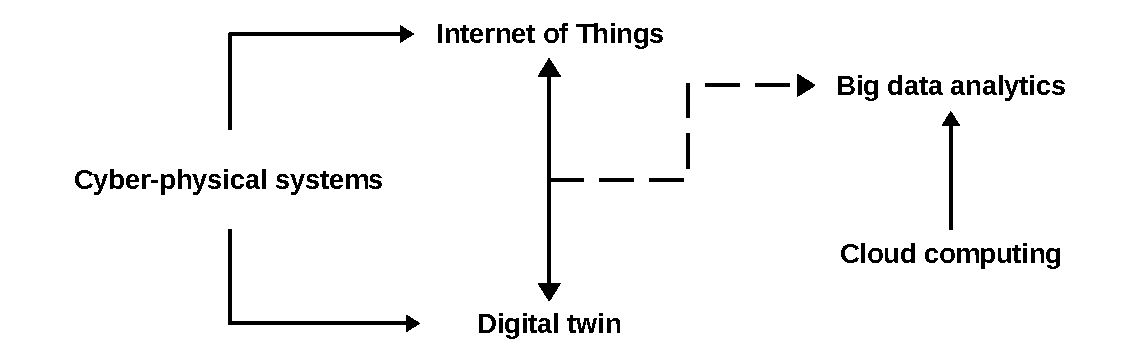
\includegraphics[width=1\textwidth]{Industria 4 schema}
\caption{Industry 4.0 scheme}
\label{fig:Industria 4 schema}
\end{figure}
Although these concepts do not have well-defined borders, and even partially overlap, figure \ref{fig:Industria 4 schema} was included to suggest a logical connection among them. The main aspect that jumps out from the previous definitions is that IoT and DT are two sides of the same coin, which is CPS: IoT can be considered the hardware side and DT the software side of a CPS. The CPS monitoring and the coordination of its parts are performed using BDA techniques, which are hosted on digital environments capable of storing and analyzing huge amount of data (i.e. CC).\\
Ultimately, information extraction and exchange are the glue that brings all the Industry 4.0 facets together. Indeed, the main innovative side that characterize the Fourth Industrial Revolution is the exploitation of huge amount of data, aiming to automatically improve efficiency and quality in manufacturing contexts. 
\section{Tools of Big Data Analytics}
BDA works as a bridge between the hardware side and the software side of a CPS, extracting information from the data collected by sensors embedded in the real system (IoT) and from data obtained by simulations run on the digital copy (DT). In general, the activity of obtaining information from big data volumes is called Knowledge Discovery in Databases (KDD), defined in \cite{ChoudharyAlokK.2009Dmim} as “\textit{the nontrivial process of identifying valid, novel, potentially useful, and ultimately understandable patterns in data}”. KDD does not belong to a specific field of application, indeed it is a framework that can also adopted in manufacturing contexts. 
\begin{figure}[h] 
\centering    
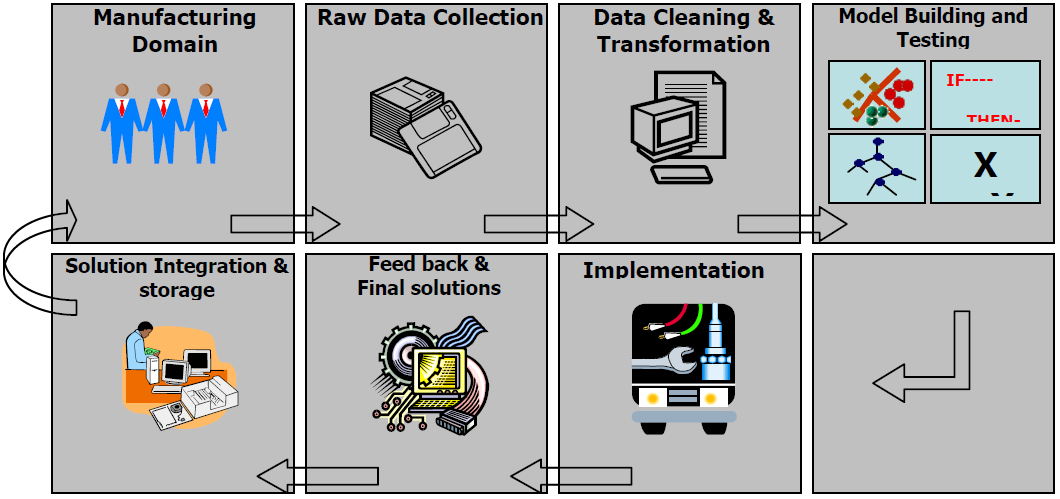
\includegraphics[width=1\textwidth]{KDD}
\caption{KDD in manufacturing \cite{ChoudharyAlokK.2009Dmim}}
\label{fig:KDD in manufacturing}
\end{figure} 
As figure \ref{fig:KDD in manufacturing} shows, KDD includes many steps: 
\begin{enumerate}
\item Understanding the manufacturing domain: preliminary research of the manufacturing sector which the data come from, and specification of the analysis goals
\item Collection of the data: raw data gathering from different sources
\item Data cleaning, pre-processing and transformation: data pre-processing to remove noise, replace missing values and redundancies, and selection of a dataset structure appropriate for data mining algorithms application 
\item Data integration: integration of data from heterogeneous sources
\item Selection of Data Mining area (see \ref{Data Mining}): selection of the Data Mining technique to use for the data analysis
\item Selection of the appropriate data mining algorithm: selection of the Data Mining algorithms to use for the data analysis
\item Interpretation and Visualization: study of the results and preparation of graphs to support the conclusions
\item Implementation of discovered knowledge: execution of the required system modifications and feedback collection 
\item Knowledge storage, reuse and integration into manufacturing system: storage of the acquired know-how in sight of future reuse
\end{enumerate}
\subsection{Data Mining}
\label{Data Mining}
The core of KDD is Data Mining (DM), that is the usage of specific algorithms for identifying patterns in data to uncover hidden relationships (Descriptive DM) and foresee outcomes (Predictive DM). It is possible to distinguish some DM main macro-areas:
\begin{itemize}
\item \textbf{Characterization \& Discrimination}: this DM branch aims to summarize data to provide a concise and information-rich description of the analyzed system. \\It is widely used in manufacturing contexts to address quality control problems or to get a overall sight of a process.
\item \textbf{Classification}: this DM branch aims to map (i.e. classify) the data into one of many different predefined classes. \\In manufacturing contexts, it is particularly used to classify defects and to perform online control chart pattern recognition.
\item \textbf{Clustering}: this DM area branch aims to map the data into one of many different not-predefined classes; these classes are called clusters, characterized by being natural grouping of data items based on similarity metrics. \\Some examples of manufacturing usage are its application to study supply chain and order picking routines, and to design part families and machine cells in cellular manufacturing.
\item \textbf{Prediction}: this DM area branch aims to build and use models to foresee the class of unlabelled samples, or to assess the value or value range of an attribute that a given sample is likely to have. \\It is widely used in manufacturing contexts, for example to design efficient resource maintenance policies, predicting the deterioration of components and machines.
\item \textbf{Association}: this DM branch aims aims to identify relationships patterns among items in a database, not based on inherent properties of the data, but rather on frequency of data-items co-occurrences. \\An example of its application in a manufacturing context is the usage of association to identify an efficient disposition of items stocked in a warehouse.
\end{itemize}
These DM macro-areas are deeply interwined and different approaches can be concurrently applied to explore data and extract meaningful information. \\
\subsection{Process Mining}
In recent years, data analysis research brought to the design of highly specialized and efficient DM algorithms, devised for specific areas of application. This leaning towards specialization lead to the definition of different DM fields, whose developments are separately pursued, even if mutual influences are still present. Some DM field examples are Text Mining, that aims to extract information from written sources, and Image Mining, that focuses on studying hidden patterns in pictures and photos. Among the others, in the late 1990s, Process Mining has been introduced.\\
Process Mining (PM) develops across multiple disciplines beyond DM, involving also Artificial Intelligence research and business process modeling. PM has the purpose of "\textit{discover, monitor and improve real processes by extracting knowledge from event logs readily available in today's (information) systems}" \cite{VanDerAalstWil2012Pmm}, where event logs are data structures that register the events occurred during a process execution (see section \ref{Event logs}). \\As the definition suggests, there are three main types of PM \cite{Aalst16}:
\begin{figure}[h]
  \centering
  \begin{subfigure}[t]{0.9\textwidth}
    
\includegraphics[width=\textwidth]{process_discovery}
    \caption{ }
    \label{fig:process_discovery}   
  \end{subfigure}
  \begin{subfigure}[h]{0.9\textwidth}
    
\includegraphics[width=\textwidth]{conformance_checking}
    \caption{ }
    \label{fig:conformance_checking}   
  \end{subfigure}
  \begin{subfigure}[b]{0.9\textwidth}
    
\includegraphics[width=\textwidth]{model_enhancement}
    \caption{ }
    \label{fig:model_enhancement}   
  \end{subfigure}
  \caption{The three main Process Mining branches, highlighting input and output of each one}
\end{figure}
\begin{itemize}
\item \textbf{Process Discovery}\\As figure \ref{fig:process_discovery} shows, this PM branch focuses on extracting information from the event log in order to understand the logical dependencies among the activities constituting the process. In other words, it aims to build a process model (i.e. a model describing the system behavior) looking at what activities are performed on cases (i.e. jobs) passing through the system.
\item \textbf{Conformance Checking}\\As figure \ref{fig:conformance_checking} shows, this PM branch focuses on the comparison of the behavior of cases registered in an event log with the process behavior prescribed in an already existing process model, looking for mismatches between the actual system (i.e. the one recorded by the event log) and theoretical system (the one represented in the model).
\item \textbf{Model Enhancement}\\As figure \ref{fig:model_enhancement} shows, this PM branch focuses on the enrichment of an already existing process model through the analysis of an event log related to the same system. In particular, the process is studied from different points-of-view, such as the resource perspective (e.g. Organizational Mining, which gives insights about the social network structure of a system) and the case perspective (e.g. time an sequence analysis, that allows to easily build Gantt Charts). 
\end{itemize}
PM has been extensively applied in business and healthcare issues \cite{RojasEric2016Pmih}, and recent researches also tried to apply it to the manufacturing context. Indeed, event logs, which are the initial data source for any PM algorithm, are obtainable as outputs of sensors embedded in production lines, making PM a promising candidate as useful tool for CPS implementation (PM can be adapted to help in the DT construction) and maintenance. In particular, concerning the second part, it is critical to design efficient methods to keep DTs aligned with the real systems, and this thesis aims to suggest a new approach and to take the first steps into a new model updating process, employing the PM framework as a starting point. 
\section{Thesis structure}
In the second chapter the thesis scope is defined, exploring the state of the art and stating the dissertation goals. The third chapter describes the study boundaries, specifying what type of manufacturing systems, sensors, and process variations are taken into account. The fourth chapter focuses on the indicators used to monitor the process, explaining how they are extracted from event logs. The fifth and sixth chapters concern the experimental tests, respectively describing the simulated system characteristics and analyzing the indicator behaviors in the simulations. The seventh chapter summarizes the results shown in the previous chapter. 
\chapter{Scope of the work}
\label{chapter 2}
\ifpdf
    \graphicspath{{Chapter2/Figs/}{Chapter2/Figs/PDF/}{Chapter2/Figs/}}
\else
    \graphicspath{{Chapter2/Figs/Vector/}{Chapter2/Figs/}}
\fi
A recently published article by Lugaresi et al. \cite{LugaresiG.2019MsmG} showed that a process model, starting from an event log, can be built using PM algorithms properly adapted to a manufacturing industry application. Thereafter, a static DT can be created using the resulting process model. However, as explained in section \ref{Industry 4.0 components}, a Digital Twin should be a dynamic copy of a real manufacturing system. It means that, ideally, the DT is changed as soon as a variation occurs in the real process, in order to keep the digital copy continuously aligned with the real system. \\
This thesis has the purpose of laying the foundation for an always up-to-date DT, making it an auto-updating copy of the real system given an initial process model. \\
\section{A standardized approach for the process model updates}
The model updating procedure, in case a variation occurs in the real system, can be divided in the three following steps.
\begin{itemize}
\item \textbf{Change detection}\\The production line is monitored to verify if a variation is occurring during the process. It is performed in real-time, computing and analyzing indicators extracted from sensor output. The continuous inspection of these indicators can be accomplished using statistical process control (SPC) techniques (e.g. Shewart Charts, Cusum Charts, EWMA Charts, Changepoint Detection), which indicate if the process behavior in a certain instant significantly differs from previous observations. So, if in the real system a variation takes place, it is possible to detect and report the change occurrence with a predetermined accuracy level, that depends on the sensor reliability and on the chosen significance level used in statistical tests. Figure \ref{fig:Model update process Detection} schematically represents a Change Detection example.
\begin{figure}[H] 
\centering    
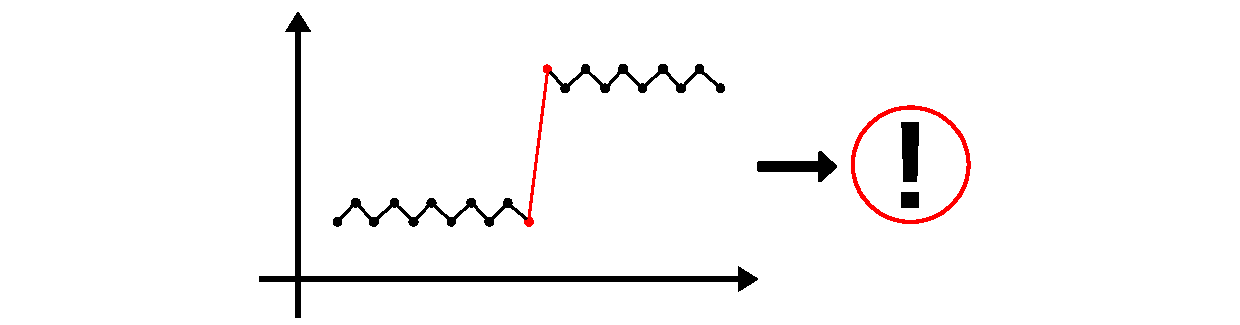
\includegraphics[width=1\textwidth]{Model update process Detection}
\caption[Model update process: Change Detection]{Change Detection: system KPIs are monitored; when a KPI variation occurrence is detected, it is reported for further analysis.}
\label{fig:Model update process Detection}
\end{figure}
\item \textbf{Change identification}\\A detected change of one or more indicators is classified to determine what kind of variation occurred in the underlying process. To do so, a “change map” is interrogated, in order to match the indicator detected change with a real system change, and then choose the correct update to the process model. Figure \ref{fig:Model update process Identification} schematically represents a Change Identification example.
\begin{figure}[H] 
\centering    
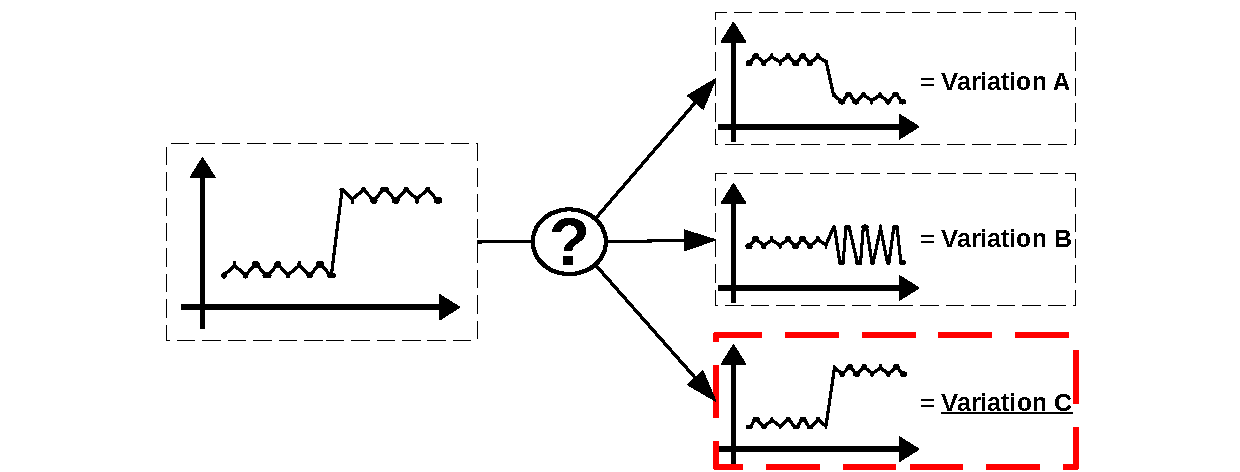
\includegraphics[width=1\textwidth]{Model update process Identification}
\caption[Model update process: Change Identification]{Change Identification: KPI variations are analyzed to identify the type of change occurred in the process.}
\label{fig:Model update process Identification}
\end{figure}
\item \textbf{Model modification}\\The process model is modified accordingly to the identified variation. A radical way to update the model is to build it from scratch, using PM algorithms, every time a variation occurs; however, in case of limited or local changes, it is not recommended to use this procedure, since the computational time and effort could be excessive. For this reason, a better approach could be the design of algorithms more specific to the occurring variation type and position, aiming to a more focused rather than a general change in the model. Figure \ref{fig:Model update process Modification} schematically represents a Model Modification example.
\begin{figure}[H] 
\centering    
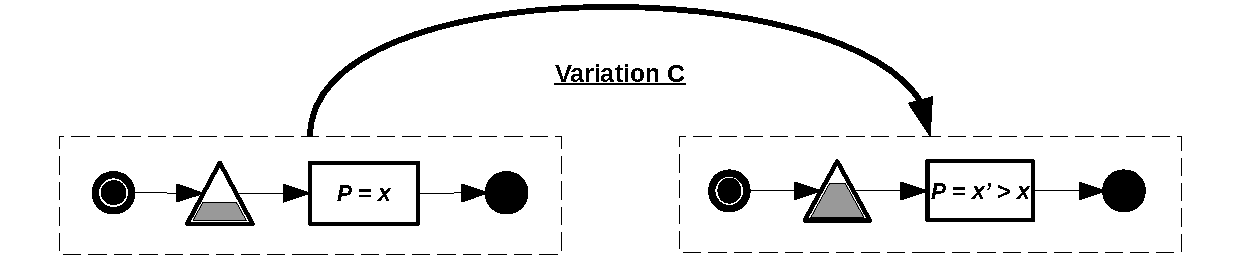
\includegraphics[width=1\textwidth]{Model update process Modification}
\caption[Model update process: Model Modification]{Model Modification: the process model is re-aligned with the real system.}
\label{fig:Model update process Modification}
\end{figure}
\end{itemize}
\subsection{Aim of the work}
\label{Aim of the work}
This thesis focuses on the second step of the model update process and, partially, on the first step. \\
Concerning the change detection, this thesis aims to answer whether or not a certain type of variation in the system is noticeable observing the monitored process indicators. Detection methods usage and even which one to apply fall outside the scope of the work. In other words, the focus is on whether a change can be detected, not on how to detect it. \\
At the same time, the thesis addresses the change identification topic, checking if it is possible to recognize the type of variation through the analysis of indicator behaviors. The main goal is to build a variation map that can be used as a guide to get insights on the process evolution. \\
This thesis is devised as part of the PM framework. In this regard, the observed indicators are extracted only from event logs generated by line sensors. The reason of this choice is to base the model update on the same data used to build the model in the first place, without requiring the addition of other sensors and the analysis of different data structures. \\
To show the novelty of this approach, the following sections are dedicated to a state of the art overview concerning the PM manufacturing applications and the PM adaptations to allow dynamic process model updates in general-purpose applications.
\section{Process Mining applications in manufacturing}
PM has been applied in manufacturing mostly as a process monitoring tool. For example, in \cite{ErMahendrawathiandArsadNovalandAstutiH.M.andPradinaRennyandUtamiRivia} PM is utilized to build the model of a production planning process of a manufacturing company using event logs obtained from an ERP system. A similar application of PM is performed in \cite{ParkMinjeongandSongMinseokandBaekTaeandSonSookyoungandHaSeungandChoSung}, where PM algorithms are adapted to analyze manufacturing make-to-order production processes, focusing on the resource workloads and on the delays caused by issues during the process. It is to be noted that, even if these studies are conducted in manufacturing contexts, they do not actually examine production lines, rather they use PM to analyze the manufacturing systems on a production planning level, and therefore are quite far from the PM application this thesis aims to achieve. \\
Lugaresi et al. in \cite{LugaresiG.2019MsmG}, as previously outlined, instead direct their attention on designing a PM algorithm which can be applied on production lines, in order to easily and swiftly build a DT imitating a real system. The mining procedure presented in the article consists of four steps:
\begin{enumerate}
\item Dataset loading: an event log is pre-filtered and pre-processed to generate the data structures suitable for the information extraction.
\item Optimized mining of event types: this is the core of the procedure, consisting in the application to data of the PM algorithm adapted to production line applications in order to obtain an \textit{activity network}, which shows how activities are connected in the system.
\item Petri Net model generation: the \textit{activity network} is translated in an initial Petri Net model\footnote{Petri Nets are process modelling language}.
\item Petri Net model adjustment: the initial Petri Net Model is polished to obtain a formally correct Petri Net model representing the real system.
\end{enumerate}
Therefore, the article shows that it is possible to mine the necessary information from a system event log to generate a process model, which can serve as a DT logical base. This thesis inserts on the same line of research, aiming to develop around this method and suggesting a procedure to move from a DT one-off generation to an always up-to-date DT.
\section{Auto-update of process models using Process Mining}
\label{Auto-update of process models using Process Mining}
In real applications, event logs often do not present as complete datasets, instead they are generated continuously appending new events recorded in real-time. In other words, an event stream is collected in an always-extending event log and there is no point in time where the dataset is finished, including the entirety of occurred events. A real-time event gathering causes challenges that basic PM algorithms are not able to deal with, since they require datasets to be finite. The PM branch that aims to address this problem is called Streaming Process Discovery (SPD), and different solutions have been developed, such as the usage of smarter forms of sampling, and summarizing the data into event frequency tables. \\
The main issue to confront when dealing with event stream is the occurrence of variations in the real system during the process. In \cite{6900341} three algorithms are proposed, aiming to build a process model from an event stream and keeping it synchronized with the system. These algorithms are based on the \textit{Heuristic Miner}, one of the most used control-flow discovery algorithms. In \cite{7376771} a similar technique is applied, introducing a growing and pruning mechanism in order to align the \textit{prefix-tree} representing the activity relationships with the real process. A different approach is taken by \cite{DennoPeterandDickersonCharlesandHardingJennifer}, where a mixed technique is designed using probabilistic neural nets and a genetic algorithm to identify and keep updated a process model with a real manufacturing system. \\
The model updating processes designed by these articles are much different from the one this thesis suggests. Indeed, in these methods models are influenced by every single event occurring in the system, without an actual monitoring of the process; instead, the approach we propose is based on the detection (and identification) of variations to trigger the model updates. Here the thesis originality lies: before model modifications we think it is critical to understand if and what kind of change is verifying in the real process, in order to minimize the updating computational effort and to be able to build a DT on more stable and reliable process models.

\chapter{Thesis boundaries}
\label{chapter 3}
\ifpdf
    \graphicspath{{Chapter3/Figs/}{Chapter3/Figs/PDF/}{Chapter3/Figs/}}
\else
    \graphicspath{{Chapter3/Figs/Vector/}{Chapter3/Figs/}}
\fi
Production systems can take a wide variety of forms, depending on the specific type of application. Generally, the proper way to explore how to address a problem using a new approach is to start from relatively simple contexts, delineating the dissertation boundaries. \\
This chapter defines the thesis areas of interest, concerning the type of production systems, the sensor positions and the types of variations assumed to occur during the process. Before the boundary definitions, a description of the event logs is provided, in order to illustrate their structure and to show what information they can carry. 
\section{Event logs}
\label{Event logs}
An event log is a data table where each row records a single event occurred during a specific process. Events are sequentially registered such that, at least, each one is associated to the case (i.e., a process instance, a job) object of the event, and with the activity (i.e., a well-defined step in the process, e.g. entering in a buffer, starting the production) performed on the case \cite{BoseR.P.JagadeeshChandra2013Wipm}. \\ 
Thus, if the event order is preserved, a minimal event log (called simple event log) is composed of only two fields, containing the following information 
\begin{itemize}
\item \textbf{ID of the case}: the code that uniquely identifies a certain case flowing in the process. 
\item \textbf{ID of the activity}: the code that uniquely identifies a certain activity performed on a case
\end{itemize}
With these three information (including the event order) a trace can be extracted for each case, which is the ordered sequence of activities executed on a case. So, a simple event log can be reorganized as a multi-set of traces over a set of activities.\\
However, in general, event logs are composed by more fields containing different case attributes or event attributes, which allow a deeper and more meaningful analysis of the process.
\begin{figure}[H] 
\centering    
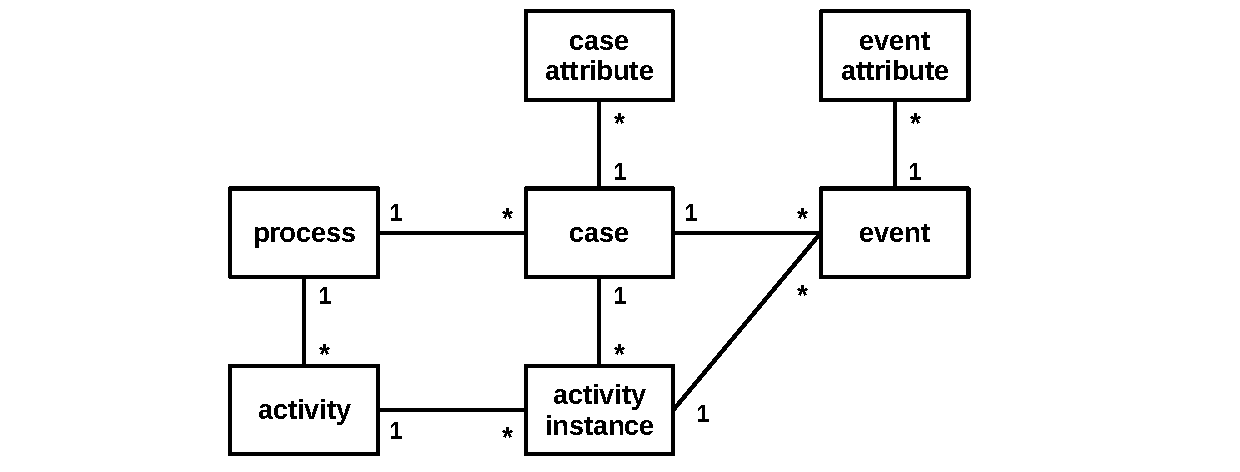
\includegraphics[width=1\textwidth]{Event_log_class_diagram_2}
\caption[Event log class diagram]{Event log class diagram \cite{Aalst16}}
\label{fig:Event log class diagram}
\end{figure}
Figure \ref{fig:Event log class diagram} displays the class diagram of the components of a general event log. The main structure of simple event logs is still present in richer event logs:
\begin{itemize}
\item Each event log refers to only one process
\item Each case belongs to one process but a process may consist of many cases
\item Each event refers to one case but a case may be the subject of many events
\item Each activity may be performed on many cases and each case may be processed by different activities
\end{itemize}
The diagram shows that, in general event logs, in contrast to simple event logs, cases and events may have many attributes. Some examples are
\begin{itemize}
\item \textbf{Timestamp}: an event attribute containing the instants when events verified
\item \textbf{ID of the resource}: an event attribute containing the codes that identify which resources (e.g. an operator that performs different activities, a machine in a multi-machine stage) were utilized to process the job
\item \textbf{Cost}: an event attribute containing the costs related to events
\item \textbf{Case type}: a case attribute registering the category to which the case belongs, useful in a multi-product system context
\end{itemize}
The presence of attributes allows to apply Model Enhancement algorithms, which aim to create models that look at a process from different perspectives. For example, if the resource ID\footnote{In this case, intended as the operator IDs} is available, it is possible to generate graphs of the social network, that show the employee relationships, the work sequence and the connection frequency. 
\subsection{Event logs in real applications: event streams}
In manufacturing, event logs are the output produced by sensors positioned along the production line. The sensor locations are determined a priori, and the sensors should guarantee a good level of reliability to minimize errors in the event log.\\
As explained in section \ref{Auto-update of process models using Process Mining}, in real applications, often, events are collected one at a time, generating event streams, however this thesis only considers event logs consisting of complete datasets, while the event stream situation is not explicitly taken into account. This simplification causes a partial, but not total, generality loss with respect to the event flow case. Indeed, this dissertation has the aim to clarify if it is possible to detect and identify some specific types of variation. Concerning the change detection, since this issue is addressed by assessing the event log with an event-by-event (or window-by-window) approach, that is comparing each new event with the previous ones, the dataset completeness is not necessary and the same approach could be also applied in an event stream context without any adaptation. Instead, regarding the change identification, the event log completeness is much more relevant. To understand what kind of variation is occurring, a simple comparison of consecutive events is insufficient, and the complete event log case and the event stream case lead to different approaches. In the first case (if the event log includes an enough long collection of after-change events), the dataset serves as a snap-shot of the process, making easy to recognize steady state periods before and after the variation and allowing to directly compare them to get insight about the process evolution. Instead, the second case, which necessarily works collecting events (or event windows) one at a time, must also deal with the problem of identifying when the process reaches again the steady state after the variation. \\
Therefore, while reasonings about the change detection can also be straight applied to event stream situations, even if the study only considers complete event logs, the change identification presents additional challenges that are not addressed in this thesis. 
\section{Considered systems}
\label{Considered systems}
\subsection{Simple serial lines (SSLs)}
In this thesis the considered systems are limited to Simple Serial Lines (SSLs), also called basic straight lines, with one resource for each of stage. 
\begin{figure}[H] 
\centering    
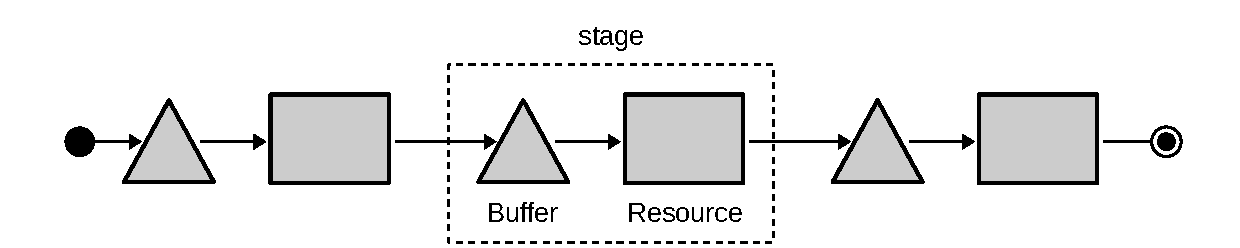
\includegraphics[width=1\textwidth]{SSL_scheme}
\caption[A SSL composed of three stages]{A SSL composed of three stages}
\label{A SSL composed of three stages}
\end{figure}
Figure \ref{A SSL composed of three stages} shows an example of a SSL made of three stages, each one composed of a buffer and a resource. SSLs are described in \cite{Romero-SilvaRodrigo2019Splp}, having the following characteristics.
\begin{itemize}
\item \textbf{Production in discrete parts}\\
Discrete manufacturing involves finished products consisting of distinct items (or batches of items) that can be counted, touched, or seen. Production is guided by a bill of materials (BOM) and follows a route, such as an assembly line. Examples of discrete manufacturing products are automobiles, furniture, and smartphones. In theory, a discrete product can be broken down at the end of its lifecycle so its basic components can be recycled.
Discrete manufacturing contrasts with process manufacturing, where the product is created by using a formula or recipe to refine raw ingredients and the final product cannot be broken down to its basic components. Examples of goods produced by process manufacturing include pharmaceuticals, food and beverages, refined oil and paints.
\item \textbf{Single type of product}\\
Multi-product systems work many types of jobs, and the job type may change during the process. Job types are distinguished, for instance, by production time or cost or because of the stage sequence that they have to pass through. SSLs process a single type of jobs, and the type does not change throughout the process.
\item \textbf{Production and transfer batches composed of one unit}\\
Resources does not process groups (i.e. batches) of jobs, but only single jobs. Moreover, jobs move from a stage to the following one alone.
\item \textbf{FIFO (First In First Out) service policy}\\
FIFO service policy\footnote{A service policy is the rule which defines the resource feeding order from the preceding buffer} prescribes that, in each stage, the first job to enter in the buffer is the first to be processed by the resource(s). The exact opposite of FIFO is LIFO (Last In First Out), which prescribes that the last job to enter in the buffer is the first to be processed by the resource. \\ It is noteworthy that, since FIFO service policy is implemented in all stages and each stage is composed by only one resource, then the job arrival order, the job process order in every stage and the job disposal order is always the same. In other words, jobs cannot swap positions after the arrival in the line. Therefore, each job is uniquely identified by its position.
\item \textbf{Not synchronized operations}\\
Each station's operation is independent from the others. The only information that a resource has access to are the fill state of the preceding buffer (i.e. the buffer in the same stage where the resource is located) and the following buffer (i.e. the buffer in the next stage). If the preceding buffer is empty, starvation occurs, that is the production stop caused by the absence of jobs to process. On the other side, if the following buffer is full, blocking occurs, that is the production stop caused by the lack of space to unload the job processed by the resource. Lack of synchronization in operations also prevents setups planning to minimize completion time. 
\end{itemize}
\subsection{Production line characteristics assumptions}
To focus on specific types of manufacturing system structures, further assumptions have been done
\begin{itemize}
\item \textbf{Production line is initially stable}\\
Stable lines are production lines where the job average arrival rate is lower than the system average service rate. In other words, mean inter-arrival time is higher than mean processing time of the bottleneck. Because of this, true bottleneck of the system is the arrival process. This assumption is made to consider a realistic production situation: an initially unstable system is clearly out-of-control since the beginning of monitoring, so it is not worth to be studied using methods that aim to find more subtle processing issues.\\
The average initial utilization in the bottleneck resource is set around 80-90\%, again to consider a realistic production condition.
\item \textbf{Production line is unsaturated and job arrival in the line is a stochastic process}\\
Unsaturated lines are production lines where the system is limited by a stochastic arrival pattern, in contrast with saturated production lines, where starvation in the first stage can never occur, meaning that the system is not dependent on material supply or incoming demand. \\
A stochastic process is a sequence of observations of the same random variable as it is observed through time. The arrival of the jobs in the line is hypothesized to follow a Poisson point process; this is a widely common assumption, since the Poisson distribution is the discrete probability distribution that expresses the probability of a given number of events occurring in a fixed interval of time if these events occur with a known constant mean rate and independently of the time since the last event. Thus, the inter-arrival time of the jobs follows an exponential distribution, which is the probability distribution of the time between events in a Poisson point process.
\item \textbf{Job processing is a stochastic process}\\
Job processing time in resources is assumed to follow a lognormal distribution, which is a continuous probability distribution of a random variable whose logarithm is normally distributed.
\item \textbf{Transfer time is negligible}\\
After being processed by a resource, jobs are sent to the buffer of the following stage. The job transfer neither uses a vehicle or an operator nor requires time to complete. So, if the buffer in the following stage is not full, the resource is released, and the processed job moves directly and immediately in the next buffer.
\item \textbf{No failures during resource process and no setups}\\
Breakdowns while the resources are processing jobs and maintenance do not occur in the considered production lines. This simplification is made to limit the sources of variability in the system to better focus on other variables. 
\item \textbf{Buffers with limited capacity}\\
Buffer capacity is limited, so when a job tries to leave a resource, if the following stage buffer is saturated, the resource is subject to blocking. An exception is the buffer in the first stage, which has never limited capacity to avoid job loss at the arrival. In chapter \ref{chapter 6} also unlimited buffers have been briefly considered (even if not realistic), to observe the effects of blocking absence on queues. Indeed, if buffers have infinite capacity, no blocking occurs and queues are influenced only by process capacity of the resource in the same stage where the buffer is placed, and by process capacity of the resource in the previous stage. Then, this simplified situation can be compared with the realistic one, where buffers are limited.
\item \textbf{Blocking after service (BAS)}\\
BAS is a resource blocking mechanism which prescribes that, after a job has been processed, if the job tries to enter in the following queue which has reached its capacity constraint, then it is forced to wait in the resource, forbidding to process the next jobs. When a space becomes available in the following buffer, the job moves, the resource is released, and service can resume.
\item \textbf{Unconstrained departures}\\
After being processed by the last stage resource, jobs leave the system freely, without any blocking mechanism.
\end{itemize}
\section{Considered sensor positions}
\label{Considered sensor positions}
To build a full functioning DT many types of sensors can be involved. For example, in \cite{ASchutze2018S4s} an IoT application in a hydraulic system is described: the outputs of different kinds of sensors (e.g. pressure sensors, flow sensors, electrical power sensors, temperature sensors, vibration sensors) are combined into calculated indicators in order to identify hydraulic system faults and defects of the sensors themselves. The same information could be used to keep a hypothetical DT aligned with the real system in every subtle detail. \\
However, a process model, which is the fundamental structure of a DT, can be built requiring much less information. Indeed, to automatically create a basic process model using PM, even simple event logs are sufficient. This kind of event logs are obtainable as output of sensors, embedded in specific places along the line, that record just the ID of the case flowing through the sensor position and the timestamp corresponding to the passage instant. Therefore, given the simple task of the sensors considered in this application, not the sensor type, but the placement choice is critical. \\
In this thesis, a placement configuration with three sensors in each stage is assumed to be implemented:
\begin{enumerate}
	\item One sensor at the buffer entrance. Since, as explained in section \ref{Considered systems}, transfer time is assumed always null, this position also corresponds to the resource exit of the previous stage.
	\item One sensor at the resource entrance, corresponding to the buffer exit.
	\item One sensor in the resource, which records job processing finish. It is to be noted that it does not coincide with the resource exit: indeed, a job could stop inside the resource if the buffer in following stage is full, because of the BAS policy.
\end{enumerate}
\begin{figure}[H] 
\centering    
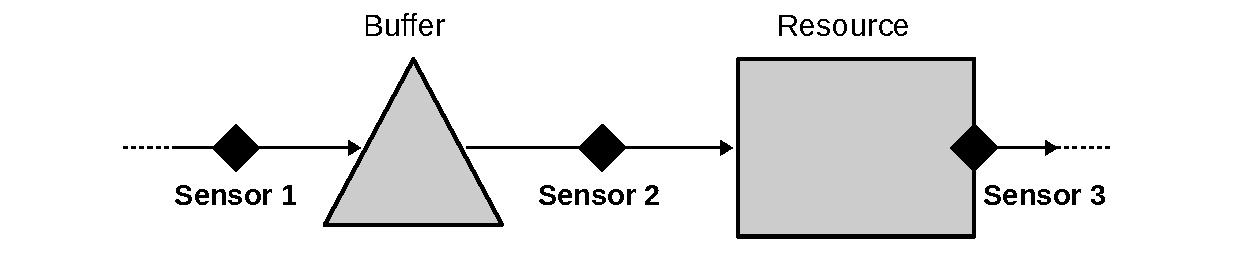
\includegraphics[width=1\textwidth]{Production_line_sensor_conf_thesis}
\caption[Three sensors configuration scheme]{Three sensors configuration scheme}
\label{fig:Three sensors configuration scheme}
\end{figure}
All the sensors are identical, and they all collect the same data, that are the job identification code (Case ID) and its passage instant (Timestamp). These are not the only fields composing the output event log, other attributes are associated, but they are not job-related fields, which have to be actively recorded by the sensors (like Case ID and timestamp), instead they keep track of the event and the sensor position. \\
%At the end of the thesis the topic of which indicators are obtainable if only two sensors are present in each stage is discussed. This situation could occur because of the breakage of one sensor or in the case of a placement design that aims to reduce time and costs related to implementation. 
\section{Considered process variations}
\subsection{Variation classifications}
The issue of process variation has been addressed in Process Mining, in particular within the wider topic of Streaming Process Discovery (see section \ref{Auto-update of process models using Process Mining}), that is the construction of models based not on finite event logs but on streams of events. Indeed, in the long term, an event stream relative to a process monitored in real time could be susceptible to concept drifts, which are “\textit{situations where the process is changing while being analyzed}” \cite{Aalst16}. \\
In \cite{BoseR.P.J.C.2011Hcdi} by Bose et al., concept drifts are classified based on three criteria. 
\subparagraph{Classification on perspective} It focuses on where the change occurs, indicating not the physical location but the level of variation. Three categories are identified:
\begin{itemize}
\item \textbf{Control-flow perspective}: this class includes structural changes, such as insertions, deletions, substitutions, and reordering of process components. For example, inserting new stages in the line, or adding new product types, cause variations of the model structure itself. 
\item \textbf{Data perspective}: this class includes changes related to requirements, usages, a data generation. For example, the enabling the execution of a task without the information request previously needed. 
\item \textbf{Resource perspective}: this class includes changes in roles and behaviors of resources. These variations influence the executions of a process, for example a resource capacity increase in the bottleneck can make the throughput increase if the process is unstable (i.e. production-constrained), or, in a multi-resource stage, a machine disabling makes the stage slower and raises its utilization.
\end{itemize}
\subparagraph{Classification on duration} As the name suggests, classification on duration aims to classify the variations based on their durations. Two categories are identified:
\begin{itemize}
\item \textbf{Momentary changes}: variation lifespans are short and may affect few activities, being not enough durable to influence the whole process. (Figure \ref{fig:Momentary change})
\item \textbf{Permanent changes}: variations lifespans are long-lasting, to the point that can be considered permanent. These changes usually affect all the process activities. (Figure \ref{fig:Permanent change})
\end{itemize}
\begin{figure}[H]
  \centering
  \begin{subfigure}[b]{0.4\textwidth}
    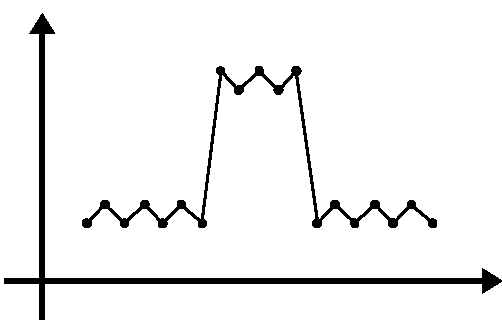
\includegraphics[width=\textwidth]{Momentary_change}
    \caption{Momentary change}
    \label{fig:Momentary change}   
  \end{subfigure}
  \hspace{0.1\textwidth}
  \begin{subfigure}[b]{0.4\textwidth}
    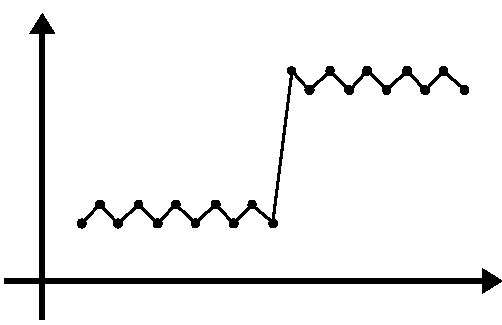
\includegraphics[width=\textwidth]{Permanent_change}
    \caption{Permanent change}
    \label{fig:Permanent change}
  \end{subfigure}             
  \caption{Change classification on duration}
  \label{fig:Change classification on duration}
\end{figure}
\subparagraph{Classification on nature} It focuses on the variation speed and frequency. Four categories are identified:
\begin{itemize}
\item \textbf{Sudden drift}: it includes variations consisting of instantaneous substitution of an existing process with a new one. This kind of change typically occurs in emergency circumstances, such as machine failures. (Figure \ref{fig:Sudden drift})
\item \textbf{Gradual drift}: it includes variations that occur without substituting the previous conditions, in other words it considers situations where different processes coexist for a certain time. This kind of variation is typical of planned organizational changes, such as the implementation of new procedures, without suddenly discontinuing the old ones. (Figure \ref{fig:Gradual drift})
\item \textbf{Incremental drift}: it includes variations that occur through small and incremental steps. This is typical of processes with slow machine deterioration over time. (Figure \ref{fig:Incremental drift})
\item \textbf{Recurring drift}: it includes variations which occur periodically, often with fixed frequency, followed by reinstatements of previous conditions. It is typical of processes characterized by seasonality. (Figure \ref{fig:Recurring drift})
\end{itemize}
\begin{figure}[H]
  \centering
  \begin{subfigure}[b]{0.4\textwidth}
    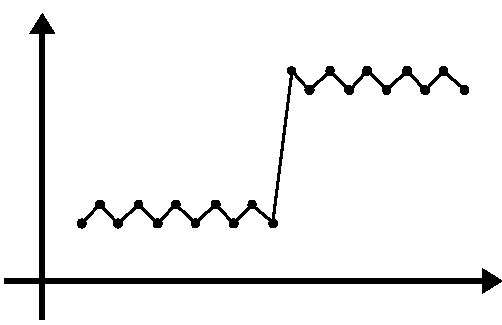
\includegraphics[width=\textwidth]{Sudden_change}
    \caption{Sudden drift}
    \label{fig:Sudden drift}   
  \end{subfigure}
  \hspace{0.1\textwidth}
  \begin{subfigure}[b]{0.4\textwidth}
    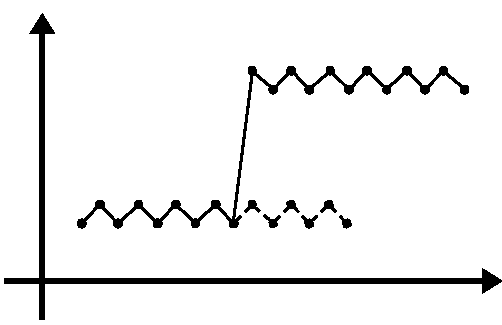
\includegraphics[width=\textwidth]{Gradual_change}
    \caption{Gradual drift}
    \label{fig:Gradual drift}
  \end{subfigure}
  \begin{subfigure}[b]{0.4\textwidth}
    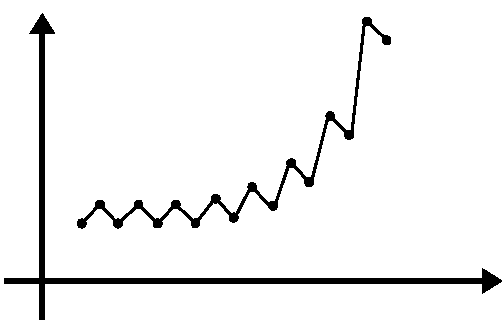
\includegraphics[width=\textwidth]{Incremental_change}
    \caption{Incremental drift}
    \label{fig:Incremental drift}
  \end{subfigure}
  \hspace{0.1\textwidth}
  \begin{subfigure}[b]{0.4\textwidth}
    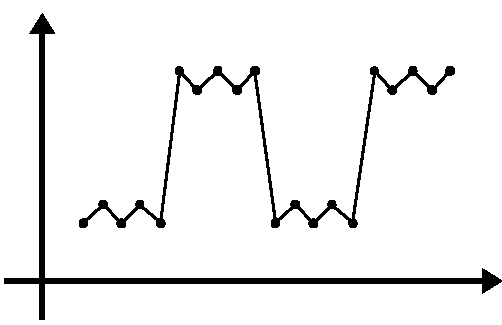
\includegraphics[width=\textwidth]{Recurring_change}
    \caption{Recurring drift}
    \label{fig:Recurring drift}
  \end{subfigure}
  \caption{Change classification on nature}
  \label{fig:Change classification on nature}
\end{figure}
\subsection{Considered variations}
In this thesis two variation types are considered:
\begin{itemize}
\item \textbf{Processing time variation in a resource}: a machine in a stage is subject to a sudden production capacity growth or loss, causing, respectively, a decrease or an increase of time needed to process a job in the stage. A capacity growth in a stage may occur in case of a machine substitution with a new and more efficient one. On the other side, a capacity loss may occur when an unnoticed resource deterioration is not adequately addressed by maintenance and abruptly affects the machine, slowing its production.
\item \textbf{Buffer capacity variation}: a buffer in a stage is subject to a sudden capacity limit growth or loss. This kind of variation may occur in a plug-and-play context, where buffers can expand or shrink based on the stage requirements, aiming to minimize blocking and starvation along the line. 
\end{itemize}
Therefore, according to the previous categorization, the variations considered in this dissertation are limited to stage-related, permanent, sudden changes. It is to be noted that the expression “stage-related” is used as the adaptation to a manufacturing context of the resource-perspective category, part of the classification on perspective. Indeed, in manufacturing the term resource is often used as synonym of machine, yet a resource-change, as meant above, can occur to any stage component, including buffers: a buffer capacity variation does not affect the model structure or the data requirement and usage, but influences stage behaviors and, so, the process execution, which is the distinctive trait of a resource-perspective variation. 
\chapter{Indicator extractions from event logs}
\label{chapter 4}
\ifpdf
    \graphicspath{{Chapter4/Figs/}{Chapter4/Figs/PDF/}{Chapter4/Figs/}}
\else
    \graphicspath{{Chapter4/Figs/Vector/}{Chapter4/Figs/}}
\fi
The identification and extraction of meaningful process indicators (i.e. Key Process Indicators, KPIs), capable of conveying useful information in a simple, concise, and not misleading way, is a critical challenge in Operations and Process Management. In this chapter, a series of KPIs are proposed as candidates to monitor a manufacturing system: the first section describes what fields are assumed to compose event logs generated by production lines, while the second section explains how event logs are transformed in \textit{case lists}, which are data structures more suitable for the suggested indicator extractions. The last section shows how these KPIs are computed starting from \textit{case lists} and provides a brief description of what they represent.
\section{Assumptions on event logs generated by production lines}
Event logs, as described in section \ref{Event logs}, have a well-defined general-purpose structure, characterized by the association of one row to each event, accompanied by a case identifier and an activity identifier, and also by a variable number of attributes. \\In the particular manufacturing application considered by this thesis, it is assumed that the sensor generated event logs are composed of five fields:
\begin{itemize}
\item \textbf{Event ID}: univocal code of the event. It is assumed that the event order sequence serves as ID of the event. Therefore, Event ID works on an ordinal scale and events are represented with indexes belonging to a set $\Theta$ whose elements are $e\in\{1,2,...,E\}$, where $E$ is number of the events occurring during the process. It is to be noted that, for this application, the information carried by Event ID is redundant, as explained in section \ref{From event logs to case lists}, so this field can be discharged without information loss. 
\item \textbf{Case ID}: univocal code of the job. Since the considered lines are SSLs, with one resource in each stage, and the service policy is BAS, as explained in section \ref{Considered systems}, no case order swap is possible, so the Case ID is equivalent to the job arrival order in the first stage of the line and to the job processing order in each stage. The job arrival order is used as ID for the jobs. Therefore Case ID works on a categorical scale and jobs are represented with indexes belonging to a set $\Gamma$ whose elements are $j\in\{1,2,...,J\}$, where $J$ is the total number of arrived (and processed) jobs in the line. 
\item \textbf{Activity ID}: univocal code of the stage where the event occurs. The definition of activity for the rest of the dissertation is slightly different from the one presented in section \ref{Event logs}: the term activity is not used to indicate a step in the work sequence, but a station in the manufacturing line. Since lines are SSLs, and so stages cannot be concurrent, the occupied position in the line stage sequence is used as identification code of the stage. Therefore, Activity ID works on a categorical scale and stages are represented with indexes belonging to a set $\Sigma$ whose elements are $s\in\{1,2,...,S\}$, where $S$ is the number of stages in the line. 
\item \textbf{Position ID}: univocal code of the position occupied by a sensor in a stage. This ID is univocal only inside a certain stage: multiple sensors in different stages own the same ID if they occupy the same relative position. Position ID works on a categorical scale and positions are represented with indexes belonging to a set $\Pi$ whose elements are $p\in\{1,2,...,P\}$, where $P$ is the number of sensors in each stage, that is three (see section \ref{Considered sensor positions}).
\item \textbf{Timestamp}: instant when the event occurred. This field works on an interval scale, where the zero value is assumed in correspondence with the process starting instant. 
\end{itemize}
\begin{table}[H]
\caption{Example of event log generated by sensors embedded in a production line}
\centering
\label{table:Example of event log}
\scalebox{0.9}{
\begin{tabular}{c c c c c}
  \toprule
  Event ID & Case ID & Activity ID & Position ID & Timestamp \\ 
  \cmidrule{1-5}
  157480 & 7500 & 1 & 1 & 106387.78 \\ 
  157481 & 7500 & 1 & 2 & 106389.37 \\ 
  157482 & 7500 & 1 & 3 & 106392.58 \\ 
  157483 & 7500 & 2 & 1 & 106392.58 \\ 
  157484 & 7500 & 2 & 2 & 106399.19 \\ 
  157485 & 7500 & 2 & 3 & 106413.20 \\ 
  157486 & 7500 & 3 & 1 & 106413.20 \\ 
  157487 & 7500 & 3 & 2 & 106413.20 \\ 
  157488 & 7500 & 3 & 3 & 106416.90 \\ 
  157489 & 7500 & 4 & 1 & 106416.90 \\ 
  157490 & 7500 & 4 & 2 & 106416.90 \\ 
  157491 & 7500 & 4 & 3 & 106423.33 \\ 
  157492 & 7500 & 5 & 1 & 106423.33 \\ 
  157493 & 7500 & 5 & 2 & 106486.05 \\ 
  157494 & 7500 & 5 & 3 & 106498.81 \\ 
  157495 & 7500 & 6 & 1 & 106498.81 \\ 
  157496 & 7500 & 6 & 2 & 106498.81 \\ 
  157497 & 7500 & 6 & 3 & 106506.34 \\ 
  157498 & 7500 & 7 & 1 & 106506.34 \\ 
  157499 & 7500 & 7 & 2 & 106506.34 \\ 
  157500 & 7500 & 7 & 3 & 106513.06 \\ 
  \bottomrule
\end{tabular}
}
\end{table}
Table \ref{table:Example of event log} is provided to show an example of the described field structure, reproducing an event log fragment limited to the trace of a job having CaseID equal to 7500. 
\section{From event logs to case lists}
\label{From event logs to case lists}
Before the indicator extractions, the event log is modified, moving from an event perspective to a case-activity perspective. The datasets obtained modifying event logs are named \textit{case lists}. This conversion is applied to simplify the successive calculations and to organize the data in a structure that better fits the stage-focused study performed through the KPI analysis. \\
A preliminary transformation is the discharge of the Event ID field. Indeed, both Timestamp and Event ID carry the same information (i.e. the event order), however they work on different measurement scales. Timestamp works on an interval scale, while Event ID operates on an ordinal scale. Event ID clearly does not convey any information regarding the time gap between events, just their order of occurrence. Thus, Timestamp is kept, since it is the richer field, and Event ID is dismissed. \\ 
The rest of the event log undergoes a pivoting operation. The Timestamp field is spread in three fields, separating time instants acquired by sensors located in different positions (recorded in Position ID) in the same stage. The resulting fields are named as follows
\begin{itemize}
\item \textbf{Timestamp\_Buffer} ($T_B$): it registers the instant when the job entered in the stage buffer, recorded in event log rows having Position ID equal to 1
\item \textbf{Timestamp\_Resource} ($T_R$): it registers the instant when the job entered in the stage resource, recorded in event log rows having Position ID equal to 2
\item \textbf{Timestamp\_End} ($T_E$): it registers the instant when the resource finished the job processing, recorded in event log rows having Position ID equal to 3
\end{itemize}
\begin{figure}[h] 
\centering    
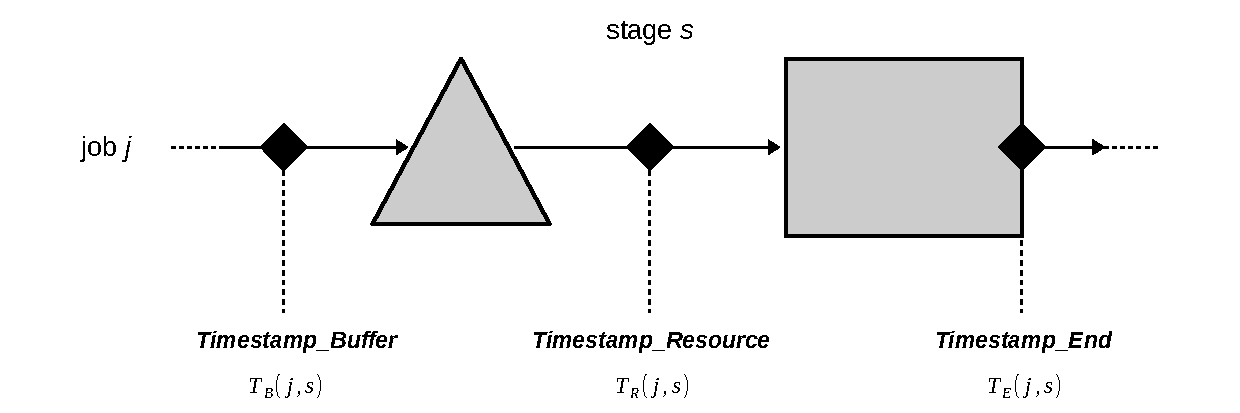
\includegraphics[width=1\textwidth]{Timestamps_thesis}
\caption[Relations between sensors and timestamps]{Relations between sensors and timestamps}
\label{fig:Relations between sensors and timestamps}
\end{figure}
Each row of the resulting dataset records the instants when the sensors in a specific stage observed the passage of a certain job. Each row is uniquely identified by (i.e. the dataset primary key is) the combination of Case ID and Activity ID. \\
For the rest of the thesis, Timestamp fields are going to be referenced as follows
\begin{itemize}
\item $T_B(j,s)$: instant of entrance of job j in the buffer of stage s
\item $T_R(j,s)$: instant of entrance of job j in the resource of stage s
\item $T_E(j,s)$: instant of processing finish of job j in stage s
\end{itemize}
\begin{table}[ht]
\caption{Example of case list}
\centering
\label{table:Example case list}
\scalebox{0.9}{
\begin{tabular}{c c c c c}
  \toprule
  Case ID & Activity ID & Timestamp\_Buffer & Timestamp\_Resource & Timestamp\_End \\ 
  \cmidrule{1-5}
  7500.00 & 1 & 106387.78 & 106389.37 & 106392.58 \\ 
  7500.00 & 2 & 106392.58 & 106399.19 & 106413.20 \\ 
  7500.00 & 3 & 106413.20 & 106413.20 & 106416.90 \\ 
  7500.00 & 4 & 106416.90 & 106416.90 & 106423.33 \\ 
  7500.00 & 5 & 106423.33 & 106486.05 & 106498.81 \\ 
  7500.00 & 6 & 106498.81 & 106498.81 & 106506.34 \\ 
  7500.00 & 7 & 106506.34 & 106506.34 & 106513.06 \\ 
  \bottomrule
\end{tabular}
}
\end{table}
Table \ref{table:Example case list} is provided to show a case list example, computed starting from the event log fragment of table \ref{table:Example of event log}.
\section{Indicator computations}
\label{Indicator computations}
Both basic and derived KPIs are calculated starting from case lists. In this section firstly the basic ones are presented, from which all the others are obtained. Then KPIs calculated aggregating on moving windows are discussed. 
\subsection{Basic KPIs}
\label{Basic KPIs}
These indicators are computed as differences between timestamps, so they are all time intervals (see figure \ref{fig:Basic KPIs scheme}). They are separated in two categories: \textbf{Same Case Intervals} (\textbf{SCI}) KPIs and \textbf{Consecutive Cases Intervals} (\textbf{CCI}) KPIs. The first category includes indicators calculated as differences of timestamps related to a specific job, not necessarily in the same stage. The second category consists of indicators calculated as differences of timestamps related to pairs of jobs consecutively passing in the same sensor position. 
\subsubsection{Same case intervals (SCI) KPIs}
\begin{figure}[H] 
\centering    
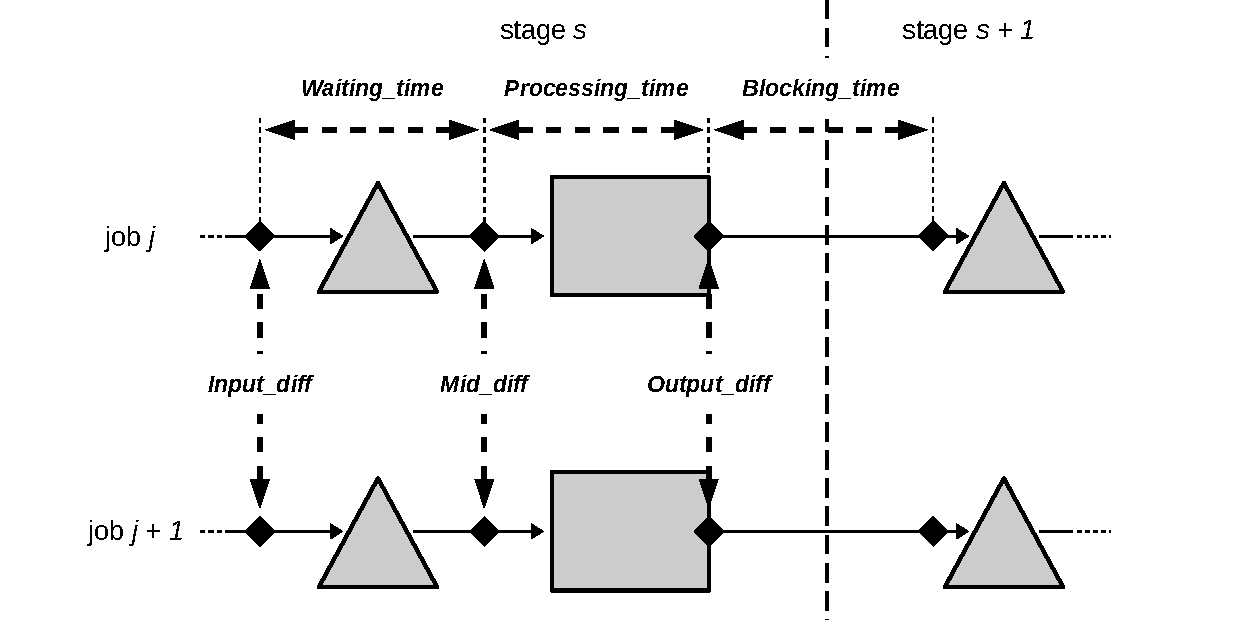
\includegraphics[width=1\textwidth]{Case_intervals_thesis}
\caption[Basic KPI computations scheme]{Basic KPI computations scheme}
\label{fig:Basic KPIs scheme}
\end{figure}
\paragraph{Waiting\_time} is a SCI indicator, computed as the difference between Timestamp\_RESOURCE and Timestamp\_BUFFER (see figure \ref{fig:Waiting time scheme}). Since Timestamp\_BUFFER is the instant when the job entered in the stage buffer, and Timestamp\_RESOURCE  is the instant when the job departed from the buffer and entered in the stage resource, this KPI represents the time spent by a job in a stage buffer. \\
The equation for Waiting\_time of job $j$ in stage $s$ is
\[Waiting\_time(j,s)=T_R(j,s)-T_B(j,s)\]
\begin{figure}[H] 
\centering    

\includegraphics[width=1\textwidth]{Same_case_intervals_WT_thesis}
\caption[Waiting time computation scheme]{Waiting time computation scheme}
\label{fig:Waiting time scheme}
\end{figure}
\paragraph{Processing\_time} is a SCI indicator, computed as the difference between Timestamp\_END and Timestamp\_RESOURCE (see figure \ref{fig:Processing time scheme}). Since Timestamp\_RESOURCE is the instant when the job entered in the stage resource (and started being processed), and Timestamp\_END is the instant when the job processing finished, this KPI represents the time spent by a job in a stage resource while being processed. \\
The equation for Processing\_time of job $j$ in stage $s$ is
\[Processing\_time(j,s)=T_E(j,s)-T_R(j,s)\]
\begin{figure}[H] 
\centering    

\includegraphics[width=1\textwidth]{Same_case_intervals_PT_thesis}
\caption[Processing time computation scheme]{Processing time computation scheme}
\label{fig:Processing time scheme}
\end{figure}
\paragraph{Blocking\_time} is a SCI indicator, computed as the difference between Timestamp\_BUFFER, registered at the entrance of the stage following the considered one, and Timestamp\_END, registered in the considered stage (see figure \ref{fig:Blocking time scheme}). Since Timestamp\_END is the instant when the job ended to be processed by the stage resource, and Timestamp\_BUFFER is the instant when the job entered in the buffer of the following stage, this KPI represents the time spent by a job in a stage resource without being processed; in other words, this is the time interval during which the resource was occupied by the job because the buffer in the following stage was full, causing stage s resource blocking. \\
The equation for Blocking\_time of job $j$ in stage $s$ is
\[Blocking\_time(j,s)=T_B(j,s+1)-T_E(j,s)\]
\begin{figure}[H] 
\centering    
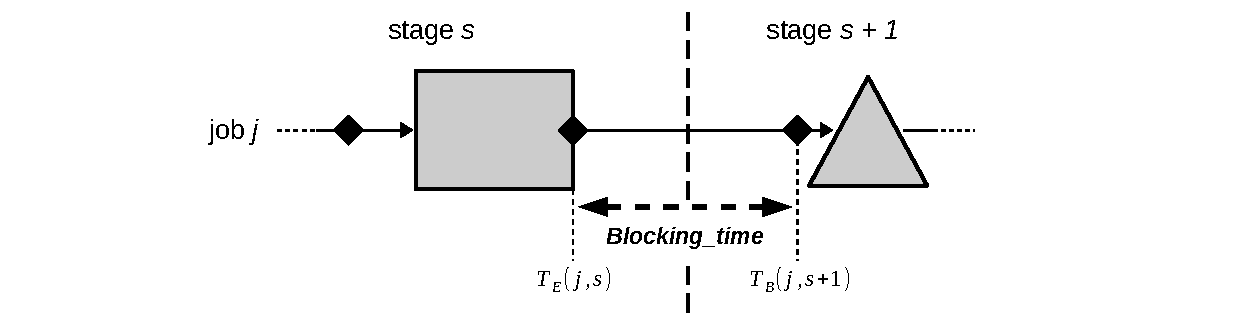
\includegraphics[width=1\textwidth]{Same_case_intervals_BT_thesis}
\caption[Blocking time computation scheme]{Blocking time computation scheme}
\label{fig:Blocking time scheme}
\end{figure}
\subsubsection{Consecutive cases intervals (CCI) KPIs}
\textbf{Input\_diff, Mid\_diff, and Output\_diff} are CCI indicators, computed as the differences between pairs of timestamps\footnote{Input\_diff is related to pairs of Timestamp\_BUFFER, Mid\_diff is related to pairs of Timestamp\_RESOURCE, and Output\_diff is related to pairs of Timestamp\_END} relative to consecutive job passages through the same sensor (see figure \ref{fig:Consecutive cases intervals scheme}). All these KPIs represent time intervals related to the cycle time as perceived by different sensor positions. The values assumed by these indicators during a process in steady state are very similar, as it is going to be shown in subsection \ref{Consecutive cases intervals KPIs - Processing time variation}. \\
The equations for CCI KPIs of job $j$ in stage $s$ are
\[Input\_diff(j,s)=T_B(j+1,s)-T_B(j,s)\]
\[Mid\_diff(j,s)=T_R(j+1,s)-T_R(j,s)\]
\[Output\_diff(j,s)=T_E(j+1,s)-T_E(j,s)\]
\begin{figure}[H] 
\centering    
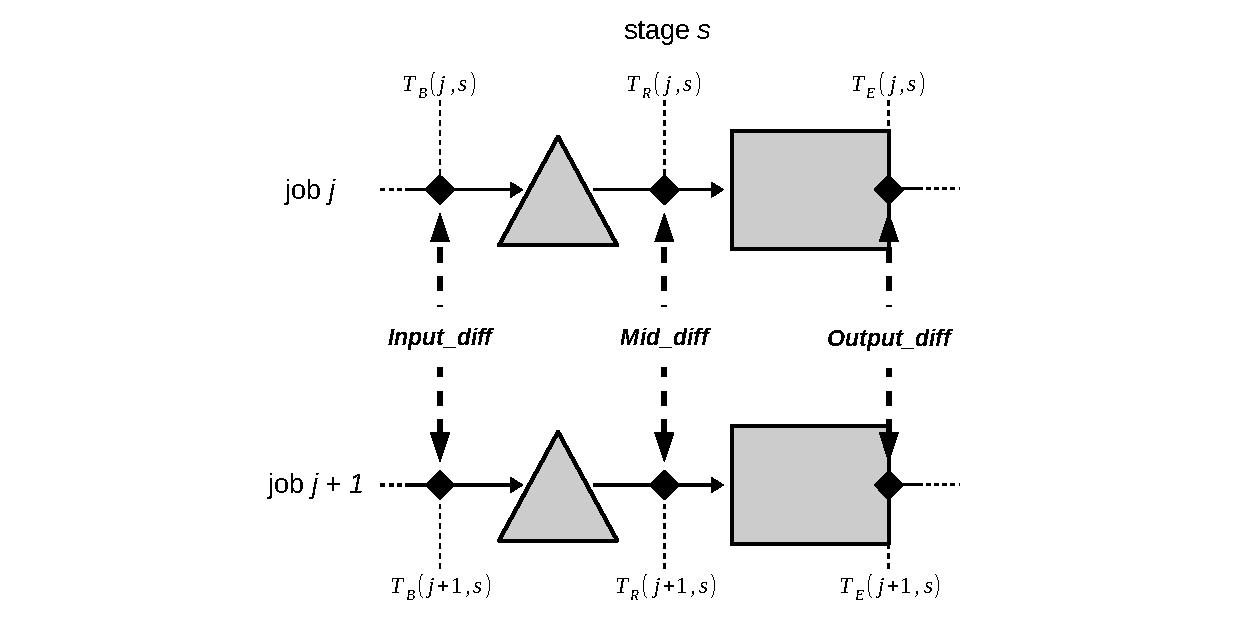
\includegraphics[width=1\textwidth]{Consecutive_cases_intervals_names_thesis}
\caption[Consecutive cases intervals computations scheme]{Consecutive cases intervals computations scheme}
\label{fig:Consecutive cases intervals scheme}
\end{figure}
\subsection{Derived KPIs}
\label{Derived KPIs}
These KPIs are obtained combining the basic KPIs introduced in the previous paragraph. The first indicator belonging to this group is called Starving\_time and it is closely related the SCI KPIs, to such an extent that is considered part of that category for the rest of the dissertation. The other derived KPIs are called Rolling Windows KPIs.
\subsubsection{Starving\_time KPI}
Starving\_time is calculated as the difference between Mid\_diff and the sum of Processing\_time and Blocking\_time (see figure \ref{fig:Starving time scheme}). As said, Mid\_diff represents the time interval between the passages of two consecutive jobs through the same sensor; this means that Mid\_diff cannot be less than Processing\_time (i.e. the time spent by a job being processed), since there is only one resource in each stage and, if the resource is seized, jobs have to wait in the buffer queue. Moreover, Mid\_diff can be greater than Processing\_time for two reasons: first, if the buffer of the following stage is full, a processed job does not release the resource, causing the machine blocking (for a period represented by Blocking\_time) and preventing other jobs to enter in the resource. Second, after a job has released the resource, if the previous buffer is empty, clearly no job seizes the resource, causing starvation. Both these resource statuses contribute to inflate Mid\_diff, that is none other than the sum of these time intervals plus the processing time. Therefore, knowing Mid\_diff, Processing\_time, and Blocking\_time, Starving\_time can be calculated and represents the time interval during which a resource was not working due to lack of jobs in the stage buffer.\\
The equation for Starving\_time of job $j$ in stage $s$ is 
\[Starving\_time(j,s)=Mid\_diff(j,s) - (Processing\_time(j,s)+Blocking\_time(j,s))\]
\begin{figure}[H] 
\centering
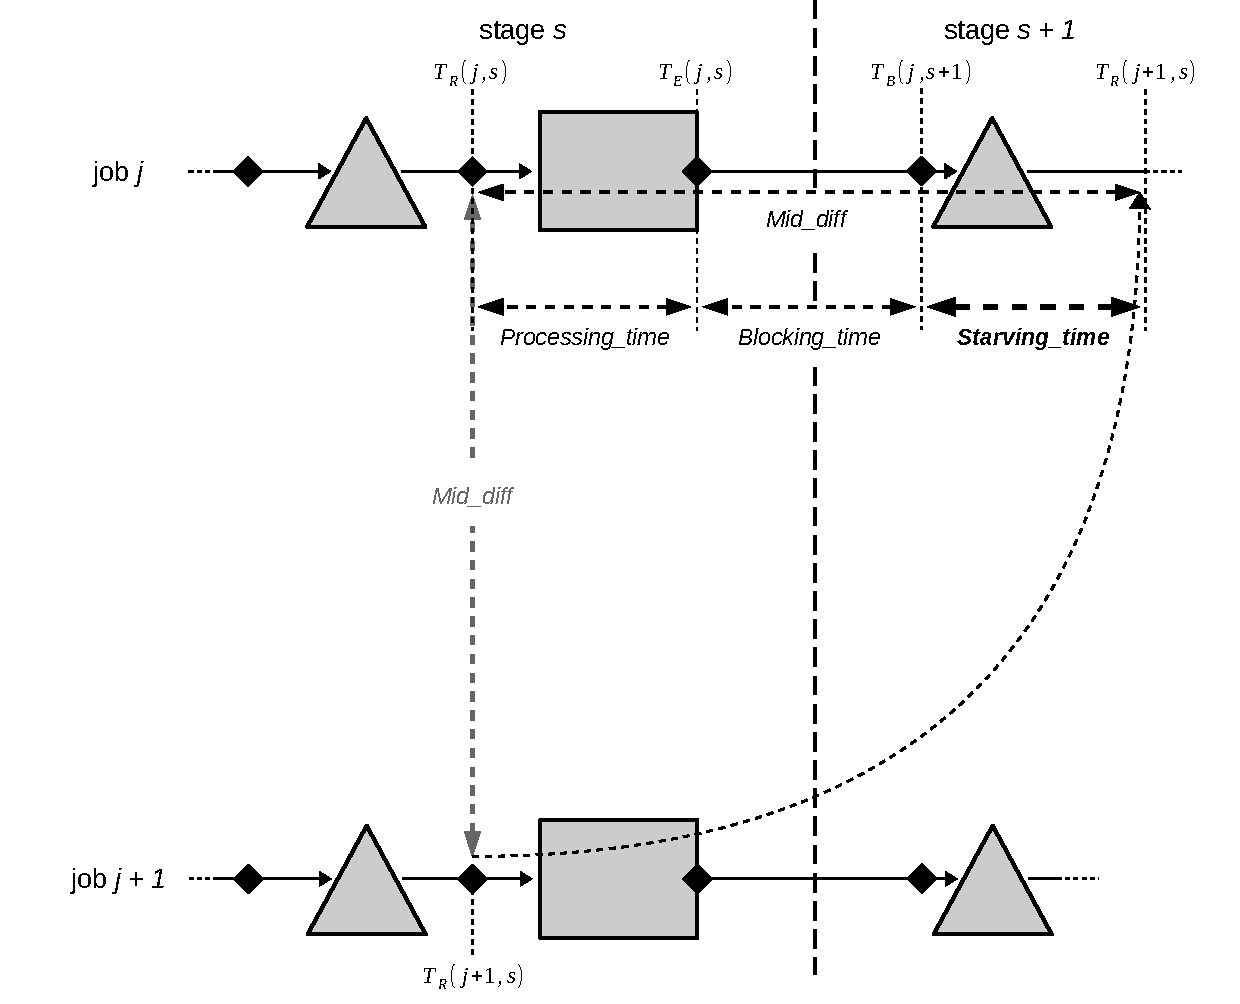
\includegraphics[width=1\textwidth]{Same_case_intervals_ST_thesis}
\caption[Starving time computation scheme]{Starving time computation scheme}
\label{fig:Starving time scheme}
\end{figure}
A more direct, yet less intuitive way to compute this KPI (found simply by replacing the basic indicators with the equations that define them) is differentiating Timestamp\_RESOURCE of the job, immediately following the considered one, entering in the stage resource, and Timestamp\_BUFFER of the considered job entering in the next stage buffer (see figure \ref{fig:Starving time formula visualization}). \\
So, an alternative formula to compute Starving\_time of job $j$ in stage $s$ is
\[Starving\_time(j,s)=T_R(j+1,s)-T_B(j,s+1)\]
\begin{figure}[H] 
\centering    
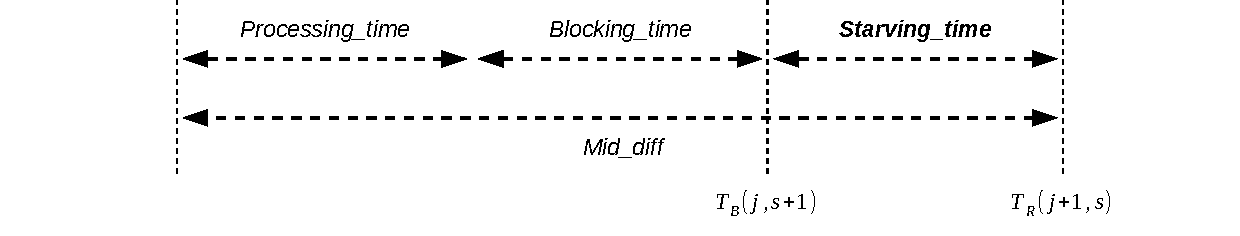
\includegraphics[width=1\textwidth]{Same_case_intervals_ST_scheme}
\caption[Starving time formula visualization]{Starving time alternative formula}
\label{fig:Starving time formula visualization}
\end{figure}
%\subsubsection{Trend KPIs}
%Trend KPIs are calculated as ratios of CCI KPIs (see figure \ref{fig:Trend KPIs scheme}). Since both numerator and denominator are time intervals, these KPIs present as absolute values. They aim to display how the job flow in a specific stage portion behaves over time. 
%\begin{figure}[H] 
%\centering    
%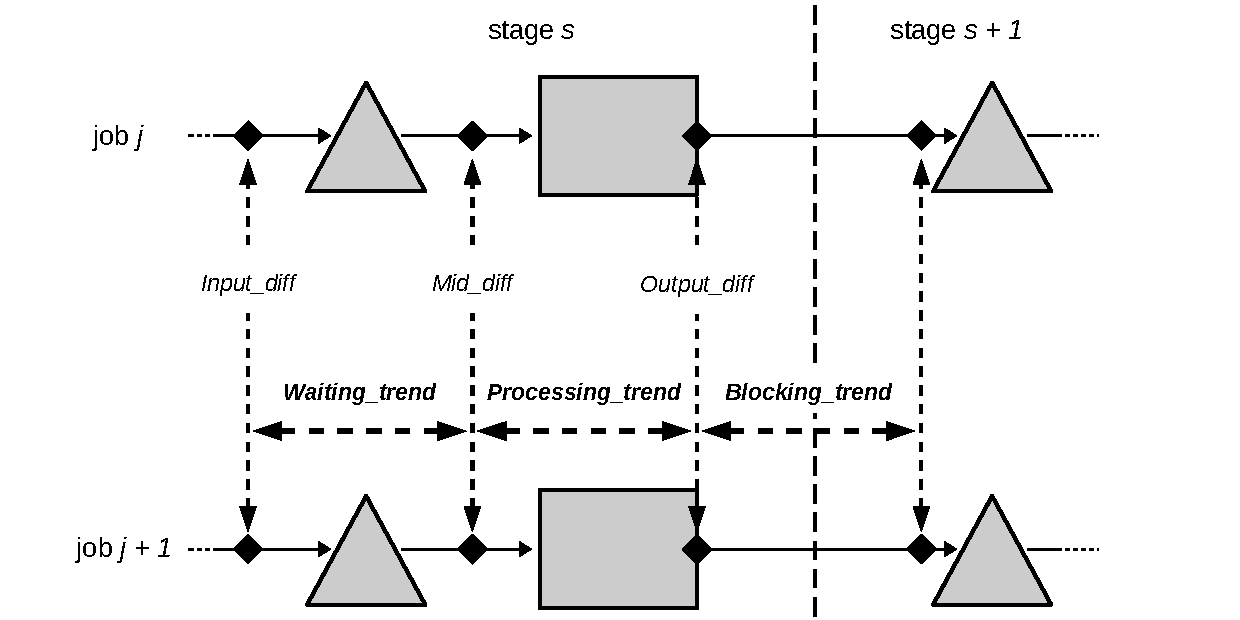
\includegraphics[width=1\textwidth]{Trend_thesis}
%\caption[Trend KPI computations scheme]{Trend KPI computations scheme}
%\label{fig:Trend KPIs scheme}
%\end{figure}
%\paragraph{Waiting\_trend} is computed as the ratio of Mid\_diff and Input\_diff both referring to the same job in the same stage. Since Mid\_diff represents the flow time at a buffer exit, and Input\_diff represents the flow time at a buffer entrance, this KPI shows if the buffer outflow is higher than the inflow or vice versa. Therefore, a greater than one Waiting\_trend (corresponding to a higher outgoing than ingoing flow time, that is a lower outgoing than ingoing flow rate) suggests that the buffer is filling up, whereas a lower than one Waiting\_trend (corresponding to a higher ingoing than outgoing flow time, that is a lower ingoing than outgoing flow rate) suggests that the buffer is emptying.\\
%The equation for Waiting\_trend of job $j$ in stage $s$ is
%\[Waiting\_trend(j,s)=\frac{Mid\_diff(j,s)}{Input\_diff(j,s)}\]
%\paragraph{Processing\_trend} is computed as the ratio of Output\_diff and Mid\_diff referring to the same job in the same stage. Since Output\_diff represents the flow time in correspondence with a job processing finish, and Mid\_diff represents the flow time at a resource entrance, this KPI shows if the resource outflow is higher than the inflow or vice versa. Therefore, a greater than one Processing\_trend (corresponding to a higher outgoing than ingoing flow time, that is a lower outgoing than ingoing flow rate) suggests that the resource is slowing down (i.e. its process capacity is reducing), whereas a lower than one Processing\_trend (corresponding to a higher ingoing than outgoing flow time, that is a lower ingoing than outgoing flow rate) suggests that the resource is accelerating (i.e. its process capacity is increasing).\\
%The equation for Processing\_trend of job $j$ in stage $s$ is
%\[Processing\_trend(j,s)=\frac{Output\_diff(j,s)}{Mid\_diff(j,s)}\]
%\paragraph{Blocking\_trend} is computed as the ratio of Input\_diff of a job in the stage following the considered one, and Output\_diff of the same job in the considered stage. Since Input\_diff represents the flow time at a buffer entrance, and Output\_diff represents the flow time in correspondence with a job processing finish, this KPI shows how blocking affects job flow. Therefore, a greater than one Blocking\_trend suggests that blocking time is increasing (i.e. resource is subject to longer blocking times), whereas a lower than one Blocking\_trend suggests that blocking time is decreasing (i.e. resource is subject to lower blocking times). 
%These indicators are quite useful, even if the carried insights are similar to the ones already offered by corresponding SCI KPIs. Indeed, as [sezione results] shows, these Trend KPIs are steadier and less noise affected, but more reactive to changes than SCI KPIs, resulting suitable to quickly detect variations in the process behavior.\\
%The equation for Blocking\_trend of job $j$ in stage $s$ is
%\[Blocking\_trend(j,s)=\frac{Input\_diff(j,s+1)}{Output\_diff(j,s)}\]
\subsubsection{Rolling Windows KPIs}
Rolling Windows (RW) KPIs are indicators calculated on case list subsection. Since this operation aggregates groups of consecutive rows (i.e. windows) in single records, the resulting dataset has as fewer rows as the subsections are wider. The table containing the aggregation results is named \textit{aggregated case list}. \\ 
RW KPIs are separated in two categories: Moment RW KPIs and Stage Metric RW KPIs. The behavior of this kind of indicators depends on the characteristics of the window which they are computed on. Indeed, windows are characterized by two parameters: length and shift. The length $l$ defines how many rows (i.e. jobs) are included in the dataset subsection. The shift $f$ defines how many rows are between the start of a subsection and the start of the following one, upper extreme included. Windows overlap if shift is lower than length ($f<l$), windows are delayed if shift is higher than length ($f>l$), windows are adjacent if the parameters are equal ($f=l$). Only complete subsections are considered (i.e. all the windows have length $l$, included the first and the last ones), and it is to be noted that the number of windows obtained from a case list varies in function of the windows parameters: the higher the shift and the length, the lower the number of windows obtained from a case list and, therefore, the fewer the rows of the aggregated case list.\\
Since each window includes $l$ jobs, it is conventionally assumed that the Case ID value of the last job $j'$ of a window serves as window ID. So, windows are represented with a set $\Omega$, a subset of set $\Gamma$, whose elements $j'$ depend on window parameters $l$ and $f$, and that includes only indexes of jobs positioned at window ends. So, given certain window parameters values, the elements of set $\Omega$ are defined through the function $j'\in\{l,l+f,l+2f,...\}\subseteq\Gamma$. 
\paragraph{Moment Rolling Windows KPIs} are RW indicators related to moments computed on case list subsections. First order moment (i.e. mean) and second order central moment (i.e. variance) are calculated for each SCI (Starving\_time included), and CCI KPI. \\
These indicators aim to reduce the noise due to process variability, and to concisely display the characteristics of the distributions followed by the related KPIs. \\
The equations for Moment Rolling RW KPIs are
\[Waiting\_time\_MEAN(j',l,f,s)=\text{mean}_j\{Waiting\_time(j,s)\}\]
\[Waiting\_time\_VAR(j',l,f,s)=\text{var}_j\{Waiting\_time(j,s)\}\]

\[Processing\_time\_MEAN(j',l,f,s)=\text{mean}_j\{Processing\_time(j,s)\}\]
\[Processing\_time\_VAR(j',l,f,s)=\text{var}_j\{Processing\_time(j,s)\}\]

\[Blocking\_time\_MEAN(j',l,f,s)=\text{mean}_j\{Blocking\_time(j,s)\}\]
\[Blocking\_time\_VAR(j',l,f,s)=\text{var}_j\{Blocking\_time(j,s)\}\]

\[Starving\_time\_MEAN(j',l,f,s)=\text{mean}_j\{Starving\_time(j,s)\}\]
\[Starving\_time\_VAR(j',l,f,s)=\text{var}_j\{Starving\_time(j,s)\}\]

\[Input\_diff\_MEAN(j',l,f,s)=\text{mean}_j\{Input\_diff(j,s)\}\]
\[Input\_diff\_VAR(j',l,f,s)=\text{var}_j\{Input\_diff(j,s)\}\]

\[Mid\_diff\_MEAN(j',l,f,s)=\text{mean}_j\{Mid\_diff(j,s)\}\]
\[Mid\_diff\_VAR(j',l,f,s)=\text{var}_j\{Mid\_diff(j,s)\}\]

\[Output\_diff\_MEAN(j',l,f,s)=\text{mean}_j\{Output\_diff(j,s)\}\]
\[Output\_diff\_VAR(j',l,f,s)=\text{var}_j\{Output\_diff(j,s)\}\]

\[Waiting\_trend\_MEAN(j',l,f,s)=\text{mean}_j\{Waiting\_trend(j,s)\}\]
\[Waiting\_trend\_VAR(j',l,f,s)=\text{var}_j\{Waiting\_trend(j,s)\}\]

\[Processing\_trend\_MEAN(j',l,f,s)=\text{mean}_j\{Processing\_trend(j,s)\}\]
\[Processing\_trend\_VAR(j',l,f,s)=\text{var}_j\{Processing\_trend(j,s)\}\]

\[Blocking\_trend\_MEAN(j',l,f,s)=\text{mean}_j\{Blocking\_trend(j,s)\}\]
\[Blocking\_trend\_VAR(j',l,f,s)=\text{var}_j\{Blocking\_trend(j,s)\}\]

Each function is computed having 
\[j\in\{j'-l+1,j'-l+2,...,j'\}\wedge j'\in\{l,l+f,l+2f,...\}\]
\paragraph{Stage State Rolling Windows KPIs} are RW indicators that help to monitor buffer and resource, exploiting the flow time to get more insights about their usage. Concerning the buffer, the average number of jobs (in a certain window) in a queue is calculated; then three resource related metrics are computed, that are utilization, probability of blocking, and probability of starvation. All Stage State RW KPIs present the same formula structure, that is the ratio between a SCI derived Moment RW KPI and a CCI derived Moment RW KPI, both calculated on the same dataset subsection. Since both numerator and denominator are time intervals, these KPIs present as absolute values. 
\subparagraph{Average\_Queue} is calculated as the ratio between the Waiting\_time\_MEAN and Input\_diff\_MEAN. Since Waiting\_time\_MEAN is the average time interval spent by jobs waiting in a buffer, and Input\_diff\_MEAN is the average time interval between consecutive jobs entering in a buffer (i.e. average flow time as seen by the buffer), their ratio tells the average number of jobs simultaneously present in a buffer.\\
The equation for Average\_Queue computed in stage $s$ on rolling windows with parameters $l$ and $f$ and having $j'$ as last job is
\[Average\_Queue(j',l,f,s)=\frac{Waiting\_time\_MEAN(j',l,f,s)}{Input\_diff\_MEAN(j',l,f,s)}\]
\subparagraph{Utilization} is calculated as the ratio between the Processing\_time\_MEAN and Mid\_diff\_MEAN. Since Processing\_time\_MEAN is the average time interval needed by a resource to process a job, and Mid\_diff\_MEAN is the average time interval between consecutive jobs entering in a resource (i.e. average flow time as seen by the resource), their ratio tells how much time the resource worked compared to the available time, or, from another point of view, the probability that, in a certain instant, the resource was not idle. \\
The equation for Utilization computed in stage $s$ on rolling windows with parameters $l$ and $f$ and having $j'$ as last job is
\[Utilization(j',l,f,s)=\frac{Processing\_time\_MEAN(j',l,f,s)}{Mid\_diff\_MEAN(j',l,f,s)}\]
\subparagraph{Blocking\_probability} is calculated as the ratio between the Blocking\_time\_MEAN and Mid\_diff\_MEAN. Since Blocking\_time\_MEAN is the average duration of a stop when blocking occurs in a resource, and Mid\_diff\_MEAN is the average time interval between consecutive jobs entering in a resource (i.e. average flow time as seen by the resource), their ratio tells how much time the resource was in a blocking state compared to the available time, or, from another point of view, the probability that, in a certain instant, the resource was blocked. \\
The mathematical equation for Blocking\_probability computed in stage $s$ on rolling windows with parameters $l$ and $f$ and having $j'$ as last job is
\[Blocking\_probability(j',l,f,s)=\frac{Blocking\_time\_MEAN(j',l,f,s)}{Mid\_diff\_MEAN(j',l,f,s)}\]
\subparagraph{Starving\_probability} is calculated as the ratio between the Starving\_time\_MEAN and Mid\_diff\_MEAN. Since Starving\_time\_MEAN is the average time a resource has to wait for the arrival of a new job after being released by the previous one, and Mid\_diff\_MEAN is the average time interval between consecutive jobs entering in a resource (i.e. average flow time as seen by the resource), their ratio tells how much time the resource was in a starving state compared to the available time, or, from another point of view, the probability that, in a certain instant, the resource was starving. \\
The equation for Starving\_probability computed in stage $s$ on rolling windows with parameters $l$ and $f$ and having $j'$ as last job is
\[Starving\_probability(j',l,f,s)=\frac{Starving\_time\_MEAN(j',l,f,s)}{Mid\_diff\_MEAN(j',l,f,s)}\]






\chapter{Simulated systems}
\label{chapter 5}

\ifpdf
    \graphicspath{{Chapter5/Figs/}{Chapter5/Figs/PDF/}{Chapter5/Figs/}}
\else
    \graphicspath{{Chapter5/Figs/Vector/}{Chapter5/Figs/}}
\fi
To observe the indicator behaviors, simulations are built to replicate a SSL having the characteristics described in section \ref{Considered systems}. Virtual sensors have been placed accordingly to the three sensor configuration shown in section \ref{Considered sensor positions}. The sensor output is an event log having the field structure defined in chapter \ref{chapter 4}.\\
Concerning the software tools: 
\begin{itemize}
\item Models are written and run with \textit{simmer} \cite{simmer}, a process-oriented discrete-event simulator.
\item Event logs transformation in case lists and KPI extractions are executed with queries mostly written with \textit{dplyr}, \textit{tidyr} and other libraries belonging to the \textit{tidyverse} collection \cite{tidyverse}.
\item Plots are printed using \textit{ggplot2}, which is also part of the \textit{tidyverse} collection.
\end{itemize}
\textit{simmer} and \textit{tidyverse} are open-source packages for \textbf{\textsf{R}} language \cite{Rlanguage}.
\section{Simulated line}
The model is designed to simulate a simple serial line having 7 stages. Each stage is composed by a resource fed by a buffer. The first buffer is supplied by a source set up to generate 10000 jobs; job inter-arrival time (i.e. inter-generation time) follows an exponential distribution with pdf
\begin{equation}
f(x;\lambda)=\begin{cases}
\lambda e^{-\lambda x}~,& \text{if}~ x\geq 0\\
0~, & \text{otherwise.}
\end{cases}
\end{equation}
having fixed parameter $\lambda=10^{-1}$. In this way, the expected value of the inter-arrival time is $\mu_{a}=10$ time units. The simulation stops when the last job has been processed by the resource in the last stage.\\ 
Job processing time in the resources follows a log-normal distribution with pdf
\begin{equation}
f(x;\mu,\sigma^2)=e^{\mu+\sigma Z(x;\mu,\sigma^2)}
\end{equation}
where $Z(x;\mu,\sigma^2)$ is the pdf of a normal distribution with mean $\mu$ and variance $\sigma^2$. The standard deviation of the log-normal distribution is set to $\sigma_s=5$ time units in every stage $s$; the initial mean is set to $\mu_s'=7$ time units in every stage, except for the resource in the bottleneck stage $s_{BN}$, where the initial mean processing time is set to $\mu_s'=8.5$.\\
During the simulation run, a variation takes place in the line, to observe how indicators behave when it occurs. The variation is realized by forcing a process parameter to suddenly change in the instant when half of the jobs (i.e. the 5000 jobs) have been processed by the first stage resource. The changing stage position $s_{CH}$ is chosen in order to have a wide view of the variation effects both upstream and downstream in the line; the change trigger was set to be sure that system was in steady state before the variation and to let it to reach the steady state again after.
\subsection{Experimental factors and levels}
In this section the experimental factors and the respective levels are presented. 
\begin{itemize}
\item \textbf{Bottleneck and changing stage positions} Bottleneck and changing stage positions in a model depend on each other. Three stage configurations are considered to observe KPIs in different situations, that are 
\begin{enumerate}
\item Bottleneck stage $s_{BN}$ is upstream the changing stage $s_{CH}$
\item Bottleneck stage $s_{BN}$ is in correspondence with the changing stage $s_{CH}$
\item Bottleneck stage $s_{BN}$ is downstream the changing stage $s_{CH}$
\end{enumerate}
So, the stage configuration pairs are
\[(s_{BN},s_{CH})\in\{(3,5),(4,4),(5,3)\}\]
\item \textbf{Initial buffer capacities} In each model, capacity limit $cl_s$ of stage $s$ buffer has the same initial value $cl_s'$ in all stages. Four initial buffer capacity levels are considered 
\begin{enumerate}
\item Buffer capacity limit equal to 3 jobs: in this configurations buffers are small and easily saturated
\item Buffer capacity limit equal to 6 jobs: in this configurations buffers are large and not commonly saturated
\item Buffer capacity limit equal to 10 jobs: in this configurations buffers are very large and almost never saturated
\item Unlimited buffers; it is to be noted that models with unlimited buffers have not been taken into account in case of buffer limit variations.
\end{enumerate}
Therefore, the before-change considered levels of $cl_s$ are (expressed in job units)
\[cl_s'\in\{3,6,10,\infty\}\]
\end{itemize}
The variation types are classified in two categories, in turn divided in two sub-categories. The considered change sizes depend on bottleneck position or initial buffer capacity of the model. Therefore, for each variation subcategory, different $cl_s$ and $(s_{BN},s_{CH})$ entail different variation levels. 
\paragraph{Processing time variation}
This type of variation is realized changing the parameter $\mu_s$ in the processing time distribution of the resource in the changing stage $s_{CH}$. The levels of the after-change value $\mu_{s_{CH}}''$ taken by parameter $\mu_{s_{CH}}$ depend on the bottleneck position in the model. A scheme of mean processing time variations is contained in Table \ref{table: Average processing time variation levels}.
\subparagraph{Processing time increase} 
\begin{itemize}
\item Bottleneck in third stage and variation in fifth stage or vice versa ($(s_{BN},s_{CH})=(3,5)\vee(5,3)$): considered mean processing time after-change values are (expressed in time units)
\[\mu_{s_{CH}}''\in\{8,9.5,11\}\]
\item Bottleneck and variation in same stage ($(s_{BN},s_{CH})=(4,4)$): considered mean processing time after-change values are (expressed in time units)
\[\mu_{s_{CH}}''\in\{9.5,11\}\]
\end{itemize}
\subparagraph{Processing time decrease}
\begin{itemize}
\item Bottleneck in third stage and variation in fifth stage or vice versa ($(s_{BN},s_{CH})=(3,5)\vee(5,3)$): considered mean processing time after-change values are (expressed in time units)
\[\mu_{s_{CH}}''\in\{4.5,6\}\]
\item Bottleneck and variation in same stage ($(s_{BN},s_{CH})=(4,4)$): considered mean processing time after-change values are (expressed in time units)
\[\mu_{s_{CH}}''\in\{4.5,6,7.5\}\]
\end{itemize}
\paragraph{Buffer capacity variation}
This type of variation is realized changing the capacity limit $cl_s$ of the changing stage $s_{CH}$ buffer. The levels of the after-change capacity buffer $cl_s''$ depend on initial buffer capacity $cl_s'$ present in the model. A scheme of buffer limit variations is contained in Table \ref{table: Buffer capacity variation levels}.
\subparagraph{Buffer capacity increase}
\begin{itemize}
\item Initial buffer capacity equal to 3 jobs ($cl_s'=3$): considered buffer capacity after-change values (expressed in job units) are
\[cl_{s_{CH}}''\in\{6,10,20\}\]
\item Initial buffer capacity equal to 6 jobs ($cl_s'=6$): considered buffer capacity after-change values (expressed in job units) are
\[cl_{s_{CH}}''\in\{10,20\}\]
\item Initial buffer capacity equal to 10 jobs ($cl_s'=10$): considered buffer capacity after-change values (expressed in job units) are
\[cl_{s_{CH}}''\in\{20\}\]
\end{itemize}
\subparagraph{Buffer capacity decrease}
\begin{itemize}
\item Initial buffer capacity equal to 3 jobs ($cl_s'=3$): considered buffer capacity after-change values (expressed in job units) are
\[cl_{s_{CH}}''\in\{1\}\]
\item Initial buffer capacity equal to 6 jobs ($cl_s'=6$): considered buffer capacity after-change values (expressed in job units) are
\[cl_{s_{CH}}''\in\{1,3\}\]
\item Initial buffer capacity equal to 10 jobs ($cl_s'=10$): considered buffer capacity after-change values (expressed in job units) are
\[cl_{s_{CH}}''\in\{1,3,6\}\]
\end{itemize}
Each factor level combination is used to build a model which is replicated 30 times, in order to assure statistical validity and accuracy in results. Therefore, every model outputs 30 event logs, that are aggregated to calculate the average Timestamp on each combination of Case ID, Activity ID and Position ID. 
\begin{landscape}
\begin{table}[p]
	\caption{Average processing time variation levels}
	\centering
	\label{table: Average processing time variation levels}
	\begin{tabular}{l c c c}
		\toprule
		\multirow{2}{*}{} & & \multicolumn{2}{c}{Stage configuration $(s_{BN},s_{CH})$}\\ 
		\cmidrule{3-4}
		& & $(4,4)$ & $(3,5)\vee(5,3)$\\ 
		\midrule
		Buffer capacity levels $cl_s'$ & & \multicolumn{2}{c}{$\{3,6,10,\infty\}$}\\
		Average before-change processing time in changing stage $\mu_{s_{CH}}'$ & & $8.5$ & $7$\\
		\midrule \midrule
		\multirow{2}{*}{Average after-change processing time in changing stage $\mu_{s_{CH}}''$} & 
		Increase $\Uparrow$ & $\{9.5,11\}$ & $\{8,9.5,11\}$\\
		& Decrease $\Downarrow$ & $\{4.5,6,7.5\}$ & $\{4.5,6\}$\\
		\bottomrule
	\end{tabular}
\end{table}
\begin{table}[p]
	\caption{Buffer capacity variation levels}
	\centering
	\label{table: Buffer capacity variation levels}
	\begin{tabular}{l c c c c}
		\toprule
		\multirow{2}{*}{} & & \multicolumn{3}{c}{Initial buffer capacity $cl_s'$}\\ 
		\cmidrule{3-5}
		& & $3$ & $6$ & $10$\\ 
		\midrule
		Stage configuration $(s_{BN},s_{CH})$ & & \multicolumn{3}{c}{$\{(3,5),(4,4),(5,3)\}$}\\
		\midrule \midrule
		\multirow{2}{*}{After-change buffer capacity in changing stage $cl_s''$} & 
		Increase $\Uparrow$ & $\{6,10,20\}$ & $\{10,20\}$ & $\{20\}$\\
		& Decrease $\Downarrow$ & $\{1\}$ & $\{1,3\}$ & $\{1,3,6\}$\\
		\bottomrule
	\end{tabular}
\end{table}
\end{landscape}
%\section{Rolling windows parameters}
%\section{Plot structure}

\chapter{Results}
\label{chapter 6}
\ifpdf
    \graphicspath{{Chapter6/Figs/}{Chapter6/Figs/PDF/}{Chapter6/Figs/}}
\else
    \graphicspath{{Chapter6/Figs/Vector/}{Chapter6/Figs/}}
\fi
This chapter aims to present a general, yet as much as possible complete collection of KPI behaviors, showing the most meaningful simulation results. Each KPI is plotted to display its behavior when a variation occurs. The graphs present all the same structure, showing the KPI values as a function of the job IDs (i.e. Case IDs). \\
For the sake of brevity, Basic KPIs plots are not discussed: the analysis would be too lengthy and dispersive, and they would be difficult to visualize since the data noise makes them barely understandable. Therefore, only RW KPIs are considered, with parameters $f = 100$ and $l = 100$. Moreover, in Processing\_time plots and CCI plots, the average inter-arrival time is displayed with a dashed line in correspondence with the value $\mu_a=10$.
\section{Processing time variation}
A processing time variation not only causes a change in Processing\_time basic and derived KPIs in correspondence with the changing stage, but also influences different KPIs in all other stages, upstream and downstream the changing stage. \\
In this section the most information-rich indicators are analyzed, starting from consecutive case intervals KPIs and their relationship with cycle time. Then, it is shown how processing time variations are directly displayed by Processing\_time. After that, the complex behavior of Blocking\_time and Starving\_time is described. Lastly, Waiting\_time and its suitability to show variations in queue lengths are presented.
\newpage
\subsection{Consecutive cases intervals KPIs}
\label{Consecutive cases intervals KPIs - Processing time variation}
Consecutive cases intervals (CCI) KPIs are indicators strongly related to the cycle time. First of all, the behavior of one of them, Mid\_diff, is shown in a processing time increase situation. Then, the stage synchronization caused by the cycle time propagation through the line is displayed with this KPI. Finally, it is shown how similar are the behaviors of Input\_diff and Output\_diff with respect to Mid\_diff.
\subsubsection{Processing time increase effects on Mid\_diff}
\begin{figure}[h] 
\centering
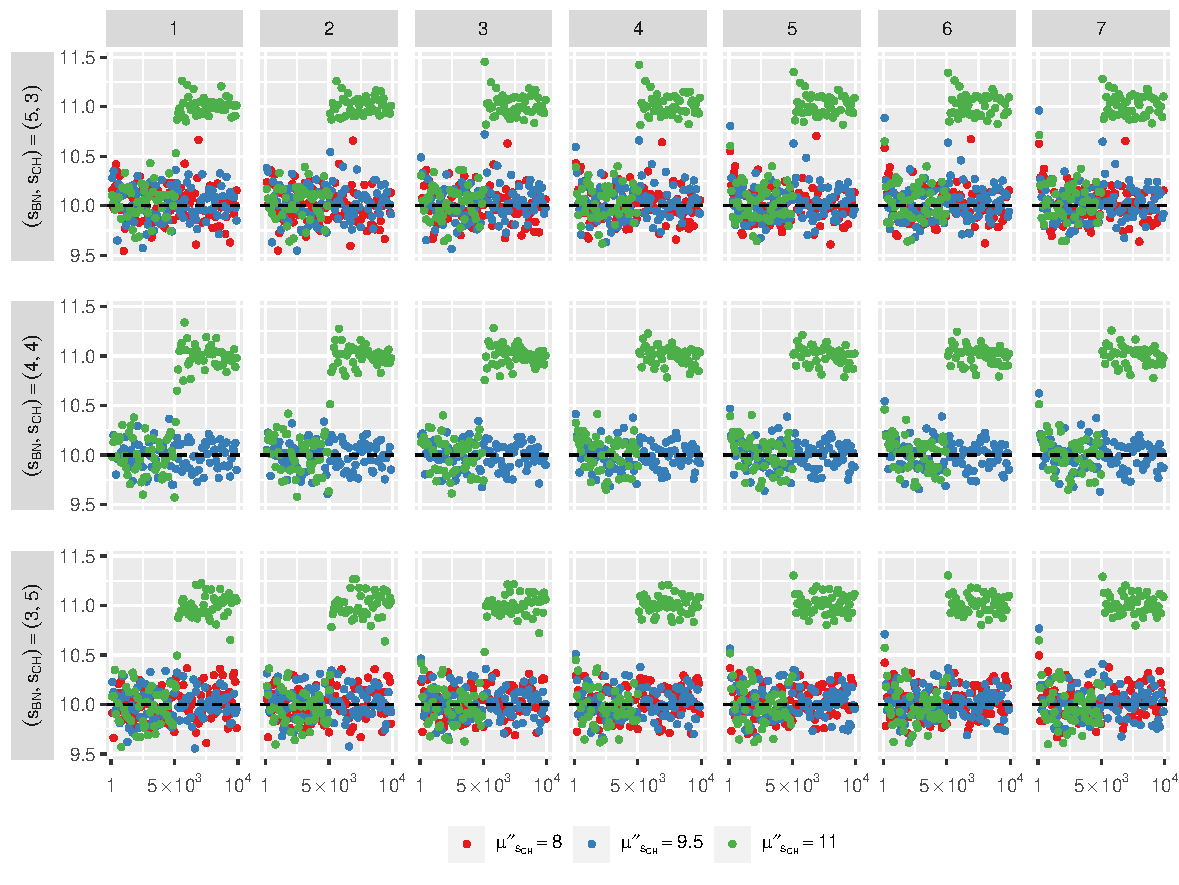
\includegraphics[width=1\textwidth]{ProcessingIncrease1_Mid_diff_MEAN}
\caption[Mid diff RW KPI behavior considering different processing time increase levels]{Mid diff RW KPI considering three mean processing time increase levels $\mu_{s_{CH}}''$ and three bottleneck - changing stage configurations $(s_{BN},s_{CH})$. Models with $cl_s=6$.}
\label{fig:Mid diff RW KPI behavior with different processing time increase levels}
\end{figure}
Figure \ref{fig:Mid diff RW KPI behavior with different processing time increase levels} shows Mid\_diff\_MEAN RW KPI behavior when a processing time growth occurs. It can be deduced that
\begin{itemize}
\item Before the variation, the system is stable and average Mid\_diff stabilizes around the average inter-arrival time $\mu_a$. \\This is visible in all the models until Case ID reaches value $5000$.
\item If a resource loses capacity, but the system remains stable (i.e. $\mu_{s_{CH}}''<\mu_a$) average Mid\_diff does not change and remains around the average inter-arrival time $\mu_a$. \\This is visible in models with $\mu_{s_{CH}}''=8$ and $\mu_{s_{CH}}''=9.5$ after Case ID has reached value $5000$.
\item If a resource loses capacity to the point that the system becomes unstable (i.e. $\mu_{s_{CH}}''>\mu_a$), average Mid\_diff increases and aligns with the bottleneck average processing time $\mu_{s_{CH}}''$. \\This is visible in model with $\mu_{s_{CH}}''=11$ after Case ID has reached value $5000$.
\item The value taken by average Mid\_diff does not depend on the stage position with respect to the changing stage $s_{CH}$ or the bottleneck $s_{BN}$: it behaves similarly in all stages. \\This is visible comparing models having different bottleneck-changing stage configurations $(s_{BN},s_{CH})$.
\end{itemize}
Mid\_diff follows the cycle time behavior as it is described in theory: it stands around a value equal to the maximum between the bottleneck average processing time $\mu_{s_{BN}}$ and the average inter-arrival time $\mu_a$\footnote{Actually, the average cycle time is equal to the maximum between the average inter-arrival time, average bottleneck processing time and average inter-departure time from the last stage, but since job departures from the system are assumed unconstrained in this thesis, the last term can be omitted.}. 
\subsubsection{Mid\_diff propagation along the line}
Even if it is scarcely visible in figure \ref{fig:Mid diff RW KPI behavior with different processing time increase levels}, Mid\_diff does not immediately change in all stages, exactly like system cycle time: when the system becomes unstable, the new cycle time needs a certain time span to spread in stages both upstream, through blocking, and downstream, through starvation. Time required to re-establish process synchronization across the line depends mainly on current saturation of buffers: the more the buffers upstream are unsaturated, the longer cycle time takes to propagate upstream (blocking is delayed). The opposite occurs for downstream stages, where cycle time spread is slower the more the buffers are saturated (starvation is delayed). 
\begin{figure}[h] 
\centering
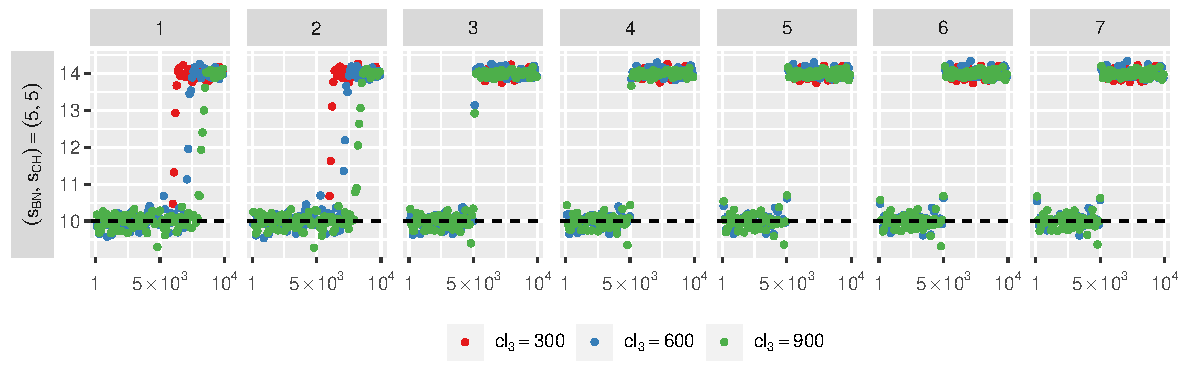
\includegraphics[width=1\textwidth]{ProcessingIncrease2_Mid_diff_MEAN}
\caption[Mid diff RW KPI variation delays considering different buffer capacity limits]{Mid diff RW KPI variation delays in case of a mean processing time increase $\mu_{s_{CH}}''$ considering different buffer capacity limits $cl_3$. Models with configuration $(s_{BN},s_{CH})=(5,3)$ and processing time increase $\mu_{s_{CH}}''=14$.}
\label{fig:Mid diff RW KPI variation delays considering different buffer capacity limits}
\end{figure}
Figure \ref{fig:Mid diff RW KPI variation delays considering different buffer capacity limits} better displays what just explained: the graphs portray a particular system where a single buffer having high capacity limit, placed in stage $s=3$, is extremely unsaturated before the variation occurs. After the first stage has processed $5000$ jobs, the resource in the bottleneck stage $s=5$, positioned downstream stage $s=3$, looses production capacity and its processing time increases to the point that it exceeds inter-arrival time and the system becomes unstable. Therefore cycle time increases, aligning with the new bottleneck average processing time, but the high capacity buffer works as a temporary decoupling point, delaying the blocking and, so, the synchronization of stages upstream its position. Moreover, these plots show that the bigger the buffer capacity ($cl_3$), the wider is the time span before cycle time (i.e. Mid\_diff) manages to spread upstream that stage.\\
This means that, a variation that has effects on CCI KPIs is immediately detectable only in correspondence of the changing stage, while in the rest of the stages the variation could be delayed due to low (or high, when cycle time spreads downstream) buffer saturation levels. 
\subsubsection{Input\_diff and Output\_diff behaviors}
\begin{figure}[h] 
\centering
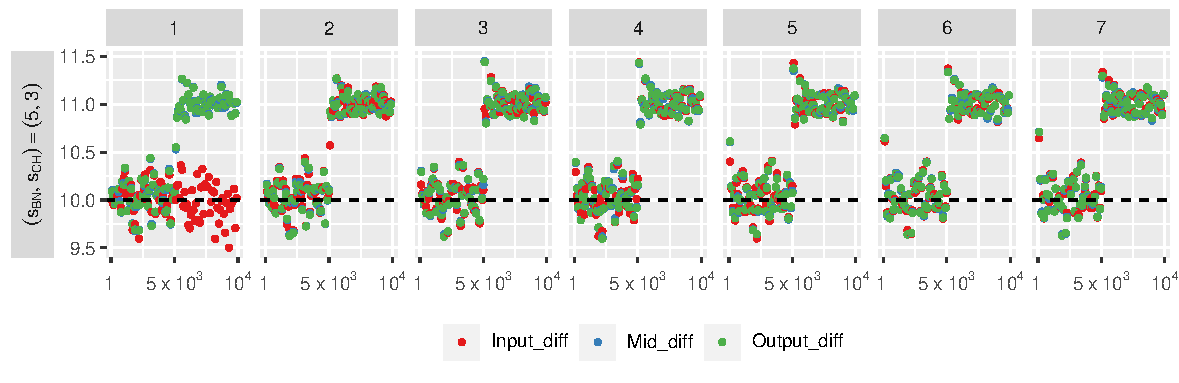
\includegraphics[width=1\textwidth]{ProcessingIncrease3_Input_diff_MEAN_Mid_diff_MEAN_Output_diff_MEAN}
\caption[Different CCI RW KPIs behaviors compared]{Different CCI RW KPIs behaviors compared . Models with configuration $(s_{BN},s_{CH})=(4,4)$, $cl_s=6$, and $\mu_{s_{CH}}''=11$.}
\label{fig:Different CCI RW KPIs behaviors compared}
\end{figure}
Input\_diff and Output\_diff behave similarly to Mid\_diff, as figure \ref{fig:Different CCI RW KPIs behaviors compared} shows. Sure enough, CCI KPIs are all indicators of cycle time as it is seen in different stage positions. However, these KPIs are not exactly equal, and Input\_diff and Mid\_diff are not interchangeable when it comes to compute Starving time and Stage State RW KPIs: since Input\_diff is relative to buffer entrances, it becomes equal to Mid\_diff, which instead is relative to buffer exits, only when the buffer is saturated and the previous resource starts to suffer of blocking. So, in general, it cannot be used to calculate the exact Starving\_time and cannot serve as denominator in Utilization, Blocking\_prob and Starving\_prob.\\
Therefore, values taken by CCI KPIs are very similar, but they differ from each other for little delays in their behaviors and generally are not exactly equal.
\subsubsection{Input\_diff in the first stage}
Since the production lines considered in this thesis always have an unlimited buffer in the first stage, Input\_diff allows to know the average inter-arrival time even when the system becomes unstable. As a matter of fact, the first buffer completely isolates the line entrance from potential system instabilities, and so Input\_diff of the first stage is actually a permanent indicator of inter-arrival time, rather than an indicator of cycle time. This detail is visible in the the first stage plot of figure \ref{fig:Different CCI RW KPIs behaviors compared}: after the variation, Mid\_diff and Output\_diff increase, while Input\_diff does not change and remains equal to the average arrival time.
\newpage
\subsection{Processing\_time and Utilization KPIs}
\label{Processing time and Utilization KPIs - Processing time variation}
Processing\_time is the most useful indicator to understand if a resource production capacity has changed and to determine its new value. In this subsection, Processing\_time behavior is analyzed in situations of processing time increase and decrease. Then, Utilization KPI is presented and its relation with Processing\_time is displayed. 
\subsubsection{Processing time increase effects on Processing\_time KPI}
\begin{figure}[h] 
\centering
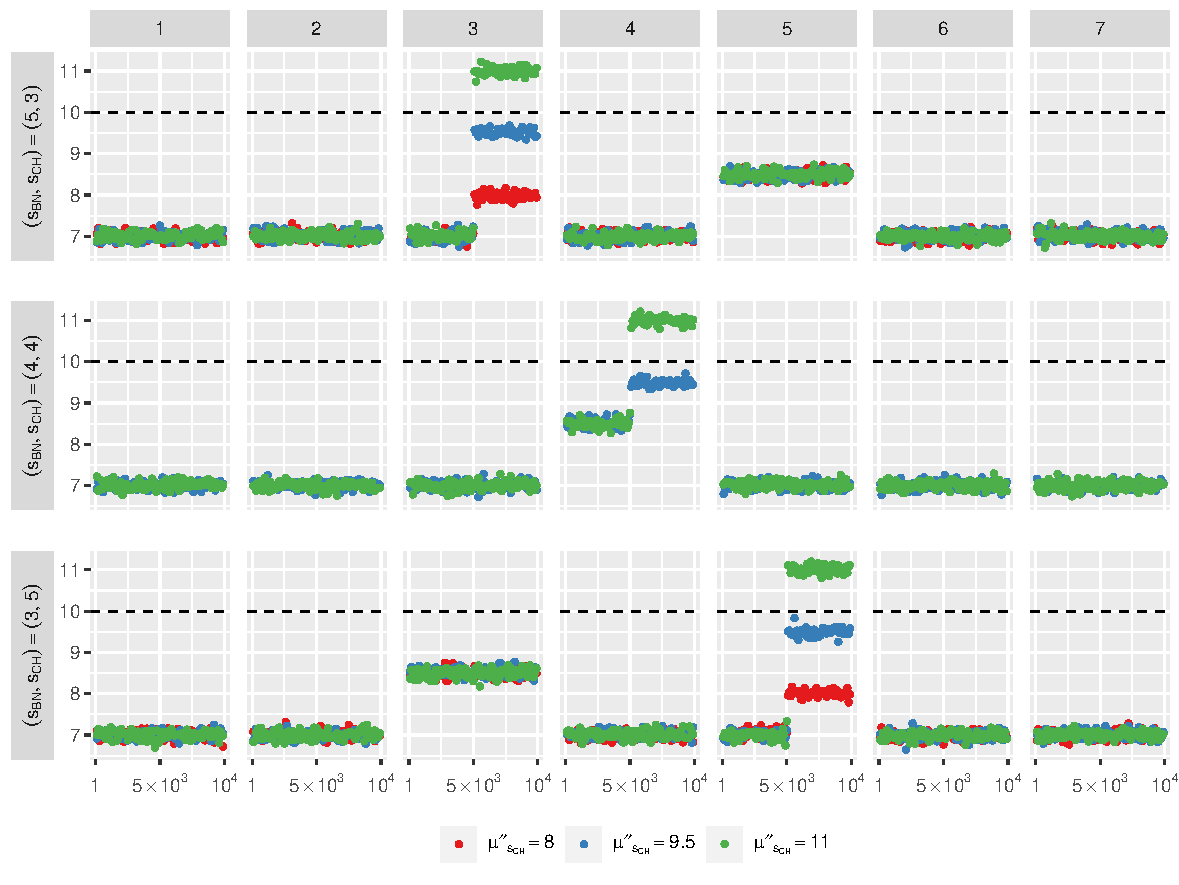
\includegraphics[width=1\textwidth]{ProcessingIncrease4_Processing_time_MEAN}
\caption[Processing time RW KPI behavior considering different processing time increase levels]{Processing time RW KPI behavior considering three mean processing time increase levels $\mu_{s_{CH}}''$ and three bottleneck - changing stage configurations $(s_{BN},s_{CH})$. Models with $cl_s=6$.}
\label{fig:Processing time RW KPI behavior with different processing time increase levels}
\end{figure}
Figure \ref{fig:Processing time RW KPI behavior with different processing time increase levels} shows Processing\_time\_MEAN RW KPI behavior when the production capacity of a stage reduces. 
\begin{itemize}
\item If a resource loses production capacity, average Processing\_time of the changing stage grows, while average Processing\_time of all other stages does not change. \\This is visible comparing the behavior of Processing\_time in correspondence with stage the changing $s_{CH}$ (where it increases) with its behavior in other stages (where it does not change). 
\item If a resource loses production capacity, the variation of changing stage average Processing\_time is such that the KPI value settles around the new average processing time of the stage. \\This is visible in each changing stage $s_{CH}$ plot. 
\item Average Processing\_time variation does not depend on the stage position with respect to the changing stage $s_{CH}$ or the bottleneck $s_{BN}$. \\This is visible comparing average Processing\_time behavior in the three different bottleneck - changing stage configurations $(s_{BN},s_{CH})$. 
\item Average Processing\_time variation does not depend on the system stability. \\This is visible comparing average Processing\_time behavior in models with $\mu_{s_{CH}}''=8$ and $\mu_{s_{CH}}''=9.5$ (where the system remains stable) with its behavior in model with $\mu_{s_{CH}}''=11$ (where the system becomes unstable).
\item Average Processing\_time of stage $s$ always stabilizes around the average time needed by stage $s$ resource to process a job. \\This is visible in all models, before and after the variation occurring when Case ID reaches value $5000$.
\end{itemize}
To summarize, the graphs show that the average Processing\_time of a stage is constantly aligned with the average processing time of that stage, even when the stage production capacity decreases. 
\subsubsection{Processing time decrease effects on Processing\_time KPI}
\begin{figure}[h] 
\centering
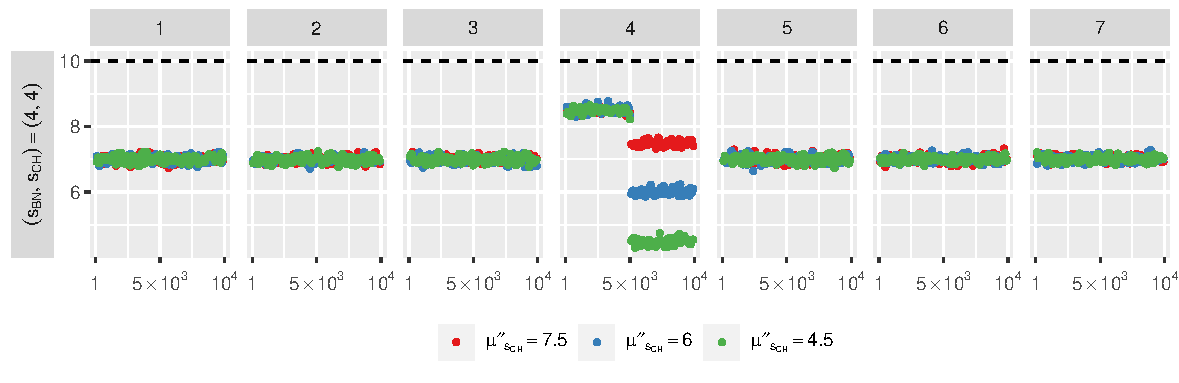
\includegraphics[width=1\textwidth]{ProcessingIncrease5_Processing_time_MEAN}
\caption[Processing time RW KPI behavior with different processing time decrease levels]{Processing time RW KPI behavior considering three different mean processing time decrease levels $\mu_{s_{CH}}$. Models with configuration $(s_{BN},s_{CH})=(4,4)$, and $cl_s=6$.}
\label{fig:Processing time RW KPI behavior with different processing time decrease levels}
\end{figure}
Figure \ref{fig:Processing time RW KPI behavior with different processing time decrease levels} shows Processing\_time\_MEAN RW KPI behavior when the production capacity of a stage increases. Looking at these plots it can be concluded that the observations made on average Processing\_time behavior in case of production capacity decrease can be extended to production capacity variations in general. Indeed, the only difference with the production capacity decrease case is that average Processing\_time of the changing stage $s_{CH}$ reduces when production capacity increases to keep aligned with the average processing time of that stage.
\subsubsection{Utilization KPI}
Processing\_time alone is useful to monitor stage production capacities, but does not give insights about how much stages work with respect to the line throughput. To obtain this information, Processing\_time\_MEAN with Mid\_diff\_MEAN are combined to calculate Utilization KPI.
\begin{figure}[h] 
\centering
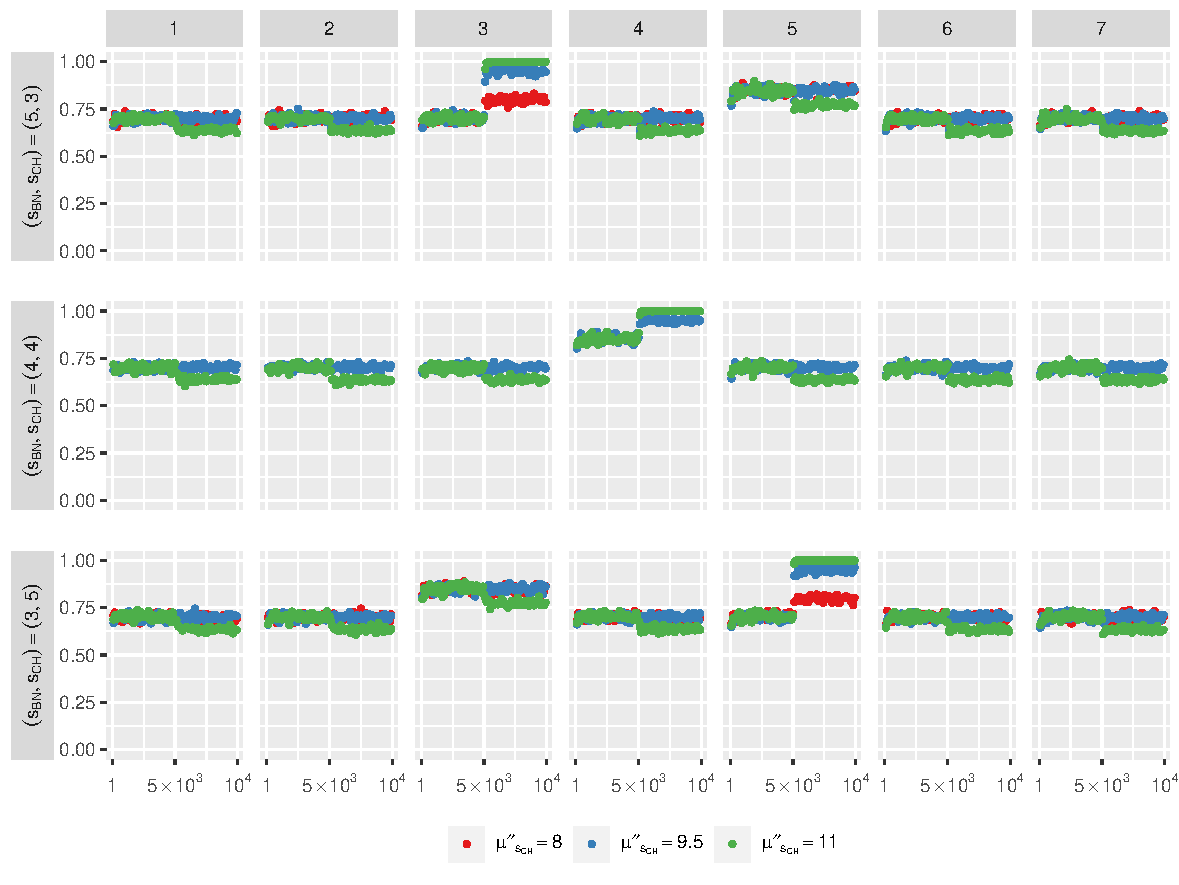
\includegraphics[width=1\textwidth]{ProcessingIncrease6_Utilization}
\caption[Utilization KPI behavior with different processing time increase levels]{Utilization KPI behavior considering three mean processing time increase levels $\mu_{s_{CH}}''$ and three bottleneck - changing stage configurations $(s_{BN},s_{CH})$. Models with $cl_s=6$.}
\label{fig:Utilization KPI behavior with different processing time increase levels}
\end{figure}
Figure \ref{fig:Utilization KPI behavior with different processing time increase levels} shows Utilization KPI behavior when the production capacity of a stage reduces. This KPI behavior is similar to average Processing\_time behavior, with some important differences
\begin{itemize}
\item If a resource loses production capacity, but the system remains stable, Utilization of the changing stage grows, while Utilization of all other stages does not change. \\This is visible in models with $\mu_{s_{CH}}''=8$ and $\mu_{s_{CH}}''=9.5$, comparing the behavior of Utilization in correspondence with stage the changing $s_{CH}$ (where it increases) with its behavior in other stages (where it does not change). 
\item If a resource loses production capacity to the point that the system becomes unstable, Utilization of the changing stage grows and settles to value $1$, while Utilization of all other stages reduces. \\This is visible in models with $\mu_{s_{CH}}''=11$, comparing the behavior of Utilization in correspondence with stage the changing $s_{CH}$ (where it increases) with its behavior in other stages (where it decreases). 
\item Utilization variation does not depend on the stage position with respect to the changing stage $s_{CH}$ or the bottleneck $s_{BN}$. This is visible comparing Utilization behavior in the three different bottleneck - changing stage configurations $(s_{BN},s_{CH})$. 
\item Values taken by Utilization are limited to the range $[0,1]$. \\This is visible in all models, before and after the variation occurring when Case ID reaches value $5000$.
\item Utilization of stage $s$ stabilizes around the average utilization of stage $s$ resource. \\This is visible in all models, before and after the variation occurring when Case ID reaches value $5000$.
\end{itemize}
Utilization KPI follows the theoretical behavior of resource utilization. Indeed, the utilization of a resource is equal to the ratio between throughput and production capacity of the resource, or in other words, it is equal to the ratio between the resource processing time and the system cycle time. Therefore, if the system becomes unstable, cycle time grows aligning with the bottleneck processing time, and so the resource utilization in the bottleneck reaches $100\%$. Instead, after all other stages have synchronized with the bottleneck lowering their throughput, their utilization reduces.\\
Even if the relative plots are not shown, it is possible to extend the observations made on Utilization behavior in case of production capacity decrease to production capacity variations in general, as with average Processing\_time. The only difference with the production capacity decrease case is that Utilization of the changing stage $s_{CH}$ reduces when production capacity increases to keep always aligned with utilization of that stage.
\newpage
\subsection{Blocking\_time, Starving\_time and respective Stage State KPIs}
\label{Blocking time, Starving time and respective Stage State KPIs - Processing time variation}
Blocking\_time and Starving\_time KPIs are analyzed together because of their strong relationship. As a matter of fact, their behavior is specular, since they both depend on the resource utilizations and on the buffer capacities. This subsection starts showing and discussing these KPI general behaviors and the effects of a processing time variation on them. Then, Bloking\_prob and Starving\_prob, which are respectively Blocking\_time and Starving\_time derived Stage State KPIs, are commented. 
\subsubsection{Processing time increase and reduction effects on Blocking\_time and Starving\_time KPIs}
\begin{figure}[h] 
\centering
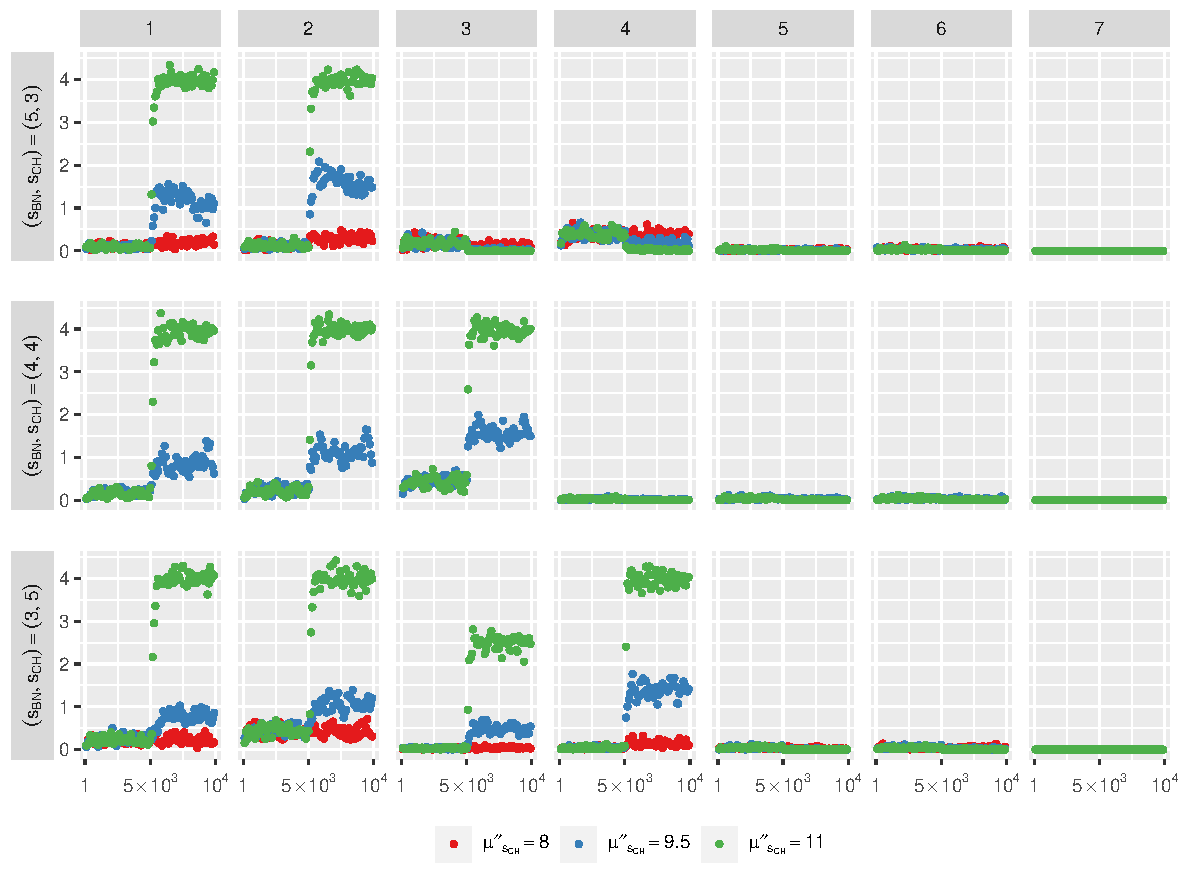
\includegraphics[width=1\textwidth]{ProcessingIncrease7_Blocking_time_MEAN}
\caption[Blocking time RW KPI behavior with different processing time increase levels]{Blocking time RW KPI considering three mean processing time increase levels $\mu_{s_{CH}}''$ and three bottleneck - changing stage configurations $(s_{BN},s_{CH})$. Models with $cl_s=6$.}
\label{fig:Blocking time RW KPI behavior with different processing time increase levels}
\end{figure}
\begin{figure}[h] 
\centering
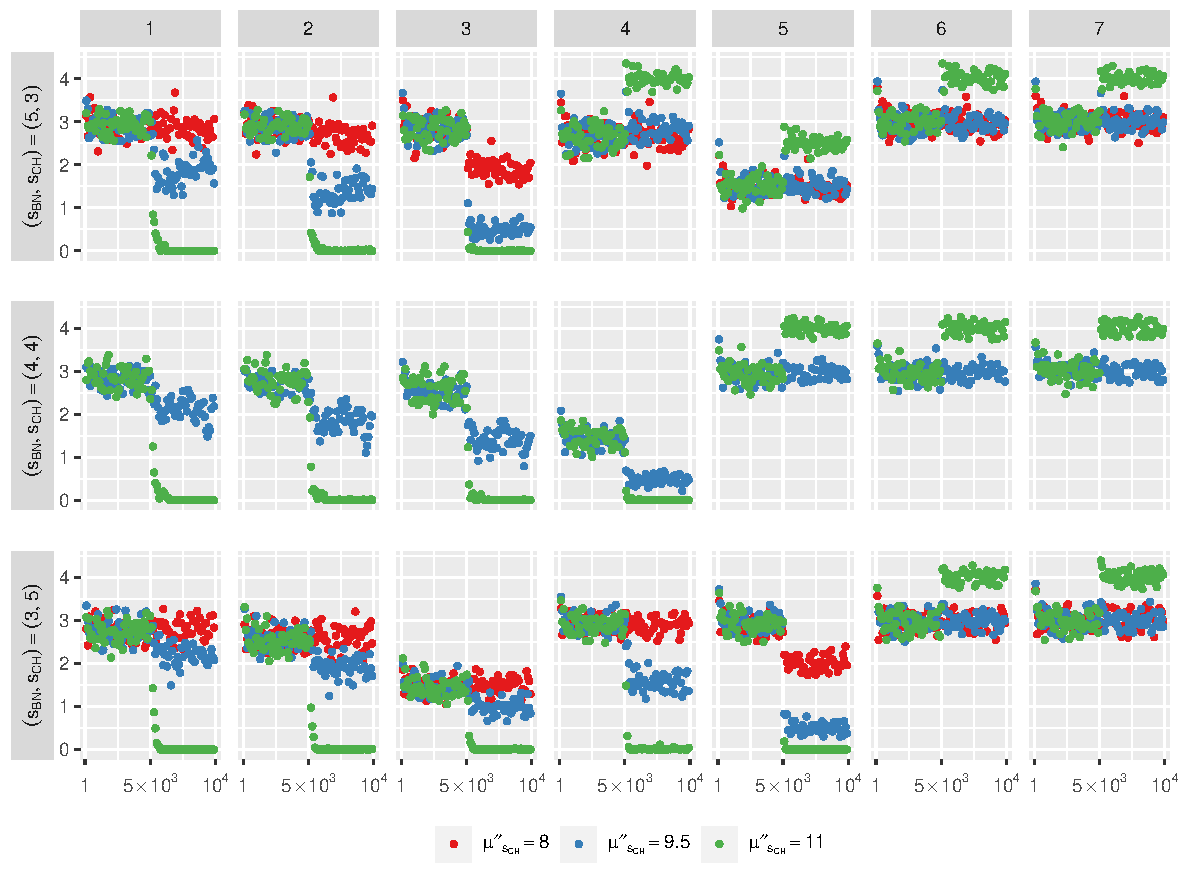
\includegraphics[width=1\textwidth]{ProcessingIncrease8_Starving_time_MEAN}
\caption[Starving time RW KPI behavior with different processing time increase levels]{Starving time RW KPI considering three processing time increase levels $\mu_{s_{CH}}''$ and three bottleneck - changing stage configurations $(s_{BN},s_{CH})$. Models with $cl_s=6$.}
\label{fig:Starving time RW KPI behavior with different processing time increase levels}
\end{figure}
Figures \ref{fig:Blocking time RW KPI behavior with different processing time increase levels} and \ref{fig:Starving time RW KPI behavior with different processing time increase levels} show, respectively, Blocking\_time\_MEAN and Starving\_time\_MEAN RW KPI behaviors when the production capacity of a stage reduces. Looking at these plots it can be said that
\begin{itemize}
\item If a resource loses production capacity to the point that the system becomes unstable:
\begin{itemize}
\item In stages upstream the changing stage $s_{CH}$, average Blocking\_time increases and settles around value $I_s$, while average Starving\_time decreases and settles around value $0$.
\item In correspondence of the changing stage $s_{CH}$, both average Blocking\_time and average Starving\_time decrease and settle around value $0$.
\item In stages downstream the changing stage $s_{CH}$, average Blocking\_time decreases and settles around value $0$, while average Starving\_time increases and settles around value $I_s$.
\end{itemize}
This is visible in models with any configuration $(s_{BN},s_{CH})$ having after-change mean processing time value $\mu_{s_{CH}}''=11$.\\
$I_s$ is equal to the difference between average Mid\_diff and average Processing\_time of stage $s$. In other words, it is a limit that depends on the cycle time as seen in stage $s$, and on stage $s$ production capacity. 
\item If a resource loses production capacity but the system remains stable:
\begin{itemize}
\item In stages upstream the changing stage $s_{CH}$, average Blocking\_time increases towards $I_s$, while average Starving\_time decreases towards $0$.
\item In correspondence of the changing stage $s_{CH}$, both average Blocking\_time and average Starving\_time decrease towards $0$.
\item In stages downstream the changing stage $s_{CH}$, average Blocking\_time decreases towards $0$, while average Starving\_time increases towards $I_s$.
\end{itemize}
This is visible in models with any configuration $(s_{BN},s_{CH})$ having after-change mean processing time value $\mu_{s_{CH}}''=8$ or $\mu_{s_{CH}}''=9.5$.
\item Average Blocking\_time and average Starving\_time variations in a certain stage $s$ are less and less relevant the further stage $s$ is from the changing stage $s_{CH}$, both upstream and downstream $s_{CH}$. 
\item Average Blocking\_time and average Starving\_Queue variations are wider the more significant is the increase of processing time.
\item Average Blocking\_time of stage $s$ stabilizes around the average time a job has to wait in stage $s$ resource after having been processed. \\Average Starving\_time of stage $s$ stabilizes around the average time passing between the exit of a job from stage $s$ resource and the entrance of a new one. \\This is visible in all models, before and after the variation occurring when Case ID reaches value $5000$.
\end{itemize}
Blocking\_time KPI and Starving\_time KPI follow the theoretical behavior of, respectively, blocking and starvation duration. Indeed, in a stable system, blocking is high in stages upstream the bottleneck, and much lower in stages downstream and in correspondence. Conversely, starvation is lower in stages upstream and in correspondence with the bottleneck, and higher downstream. When the system becomes unstable, blocking and starvation behaviors are led to the extreme 
\begin{itemize}
\item Upstream the bottleneck, when buffers become saturated, blocking causes a delay in resource releases, that last until the bottleneck has finished to process a job; so, blocking duration of a certain resource is equal to the time difference between the processing finish of a job in the bottleneck and the processing finish of a job in the considered stage. \\Downstream the bottleneck, since buffers tend to be completely empty, blocking duration drops to $0$.
\item Downstream and in correspondence of the bottleneck, starvation causes resources idleness until the bottleneck has finished to process a job; starvation lasts, like blocking upstream, the time difference between the processing end in the bottleneck and the processing end in the considered stage. \\Upstream the bottleneck, since buffers tend to be completely full, starvation duration drops to $0$.
\end{itemize}
All the observations that have been done regarding these KPIs considering production capacity reductions are similarly valid also in case of production capacity growths.
\begin{figure}[h] 
\centering
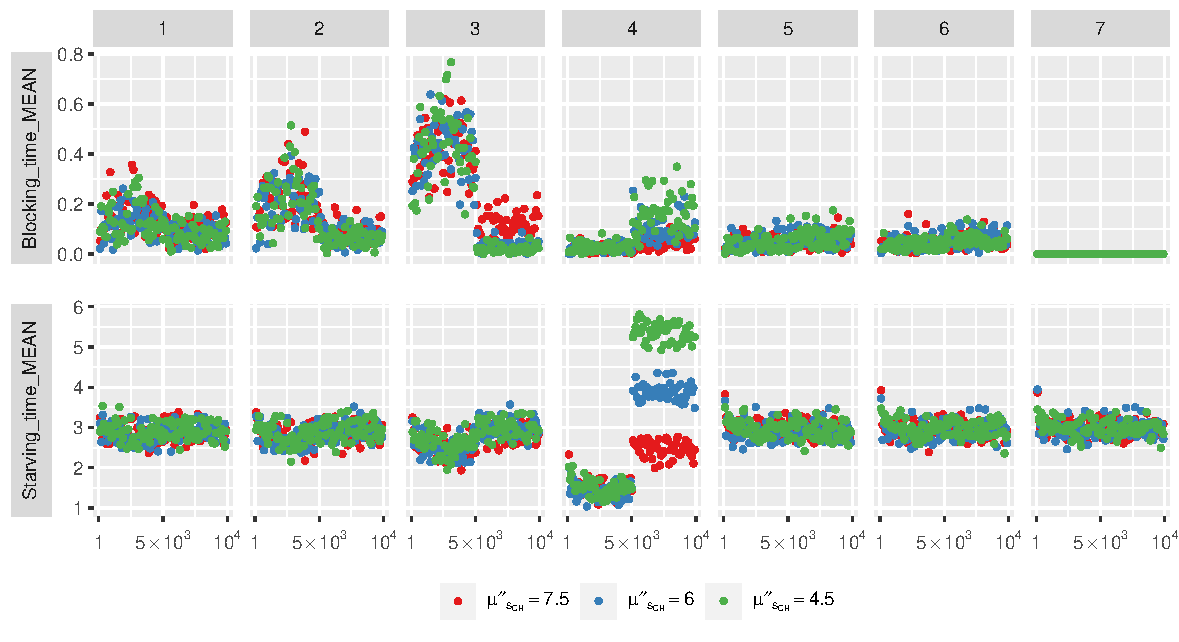
\includegraphics[width=1\textwidth]{ProcessingIncrease11_Blocking_time_MEAN_Starving_time_MEAN}
\caption[Blocking time and Starving time KPI behaviors with different processing time decrease levels]{Blocking time and Starving time KPI behaviors considering three different mean processing time decrease levels $\mu_{s_{CH}}''$. Models with configuration $(s_{BN},s_{CH})=(4,4)$ and $cl_s=6$.}
\label{fig:Blocking time and Starving time KPIs behavior with different processing time decrease levels}
\end{figure}
Figure \ref{fig:Blocking time and Starving time KPIs behavior with different processing time decrease levels} displays average Blocking\_time and average Starving\_time in case a resource processing time decreases. The only difference with the processing time increase case is that average Blocking\_time and average Starving\_time behaviors are inverted when the variation occurs:
\begin{itemize}
\item In stages upstream the changing stage $s_{CH}$, average Blocking\_time decreases, while average Starving\_time increases.
\item In correspondence of the changing stage $s_{CH}$, both average Blocking\_time and average Starving\_time increase.
\item In stages downstream the changing stage $s_{CH}$, average Blocking\_time increases, while average Starving\_time decreases.
\end{itemize}
\subsubsection{Blocking\_time and Starving\_time KPIs considering different buffer levels}
Previously only one buffer capacity limit ($cl_s=6$) was taken into account in the analysis. However, Blocking\_time and Starving\_time KPIs are also influenced by the buffer capacity, and it is interesting to study their behavior considering different capacity levels.
\begin{figure}[h] 
\centering
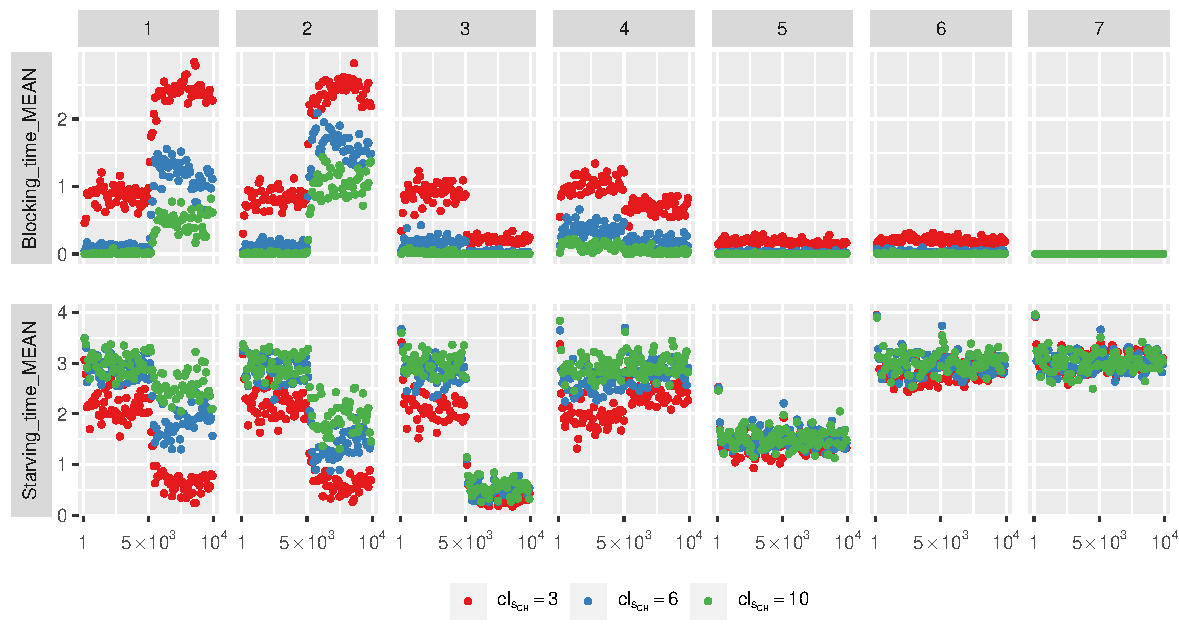
\includegraphics[width=1\textwidth]{ProcessingIncrease9_Blocking_time_MEAN_Starving_time_MEAN}
\caption[Blocking time and Starving time RW KPIs behaviors in case of processing time increase considering different buffer capacity limits]{Blocking time and Starving time RW KPI behaviors in case of mean processing time increase $\mu_{s_{CH}}''$ considering different buffer capacity limits $cl_s$. Models with configuration $(s_{BN},s_{CH})=(5,3)$ and $\mu_{s_{CH}}''=9.5$.}
\label{fig:Blocking time and Starving time RW KPIs behavior in case of processing time increase considering different buffer capacity limits}
\end{figure}
Figure \ref{fig:Blocking time and Starving time RW KPIs behavior in case of processing time increase considering different buffer capacity limits} shows average Blocking\_time and average Starving\_time behaviors in case of a processing time increase, but considering models having three different buffer capacity limits $cl_s$. \\
When a stage loses production capacity:
\begin{itemize}
\item The variation extents of average Blocking\_time and average Starving\_time are wider the lower the buffer capacity limit is
\item The variation extents of average Blocking\_time and average Starving\_time are narrower the higher the buffer capacity limit is
\end{itemize}
It is particularly visible comparing the model with $cl_s=3$ and the one with $cl_s=6$. \\
This happens because smaller buffers are on average easily saturated, causing longer resource blockings in previous stages and reducing starvation. When buffers are bigger the opposite verifies.
\subsubsection{Value $I_s$ behavior and Blocking\_time and Starving\_time relative proportions}
It is noteworthy to explain that value $I_s$ \footnote{Remember that $I_s$ was defined as the difference between average Mid\_diff and average Processing\_time of stage $s$} is not simply a superior limit for average Blocking\_time or average Starving\_time, but actually it is always equal to their sum. As a matter of fact, the sum of Blocking\_time and Starving\_time of stage $s$ is always equal to the difference between Mid\_diff and Processing\_time of stage $s$ because of how these KPIs are defined (see subsection \ref{Derived KPIs}). 
\[Blocking\_time(j,s)+Starving\_time(j,s)=Mid\_diff(j,s)-Processing\_time(j,s)\]
Theoretically, this is reasonable given the characteristics of the considered systems: since machine breakdowns are assumed to never occur, resources can find themselves in three possible states, which are seized and working state (processing), seized and not working state (blocking), and not seized state (starvation). Sum of the total time spent by a resource in these states gives the whole available time of the resource, as, analogously, Processing\_time, Blocking\_time, and Starving\_time add up matching Mid\_diff. 
\begin{figure}[h] 
\centering
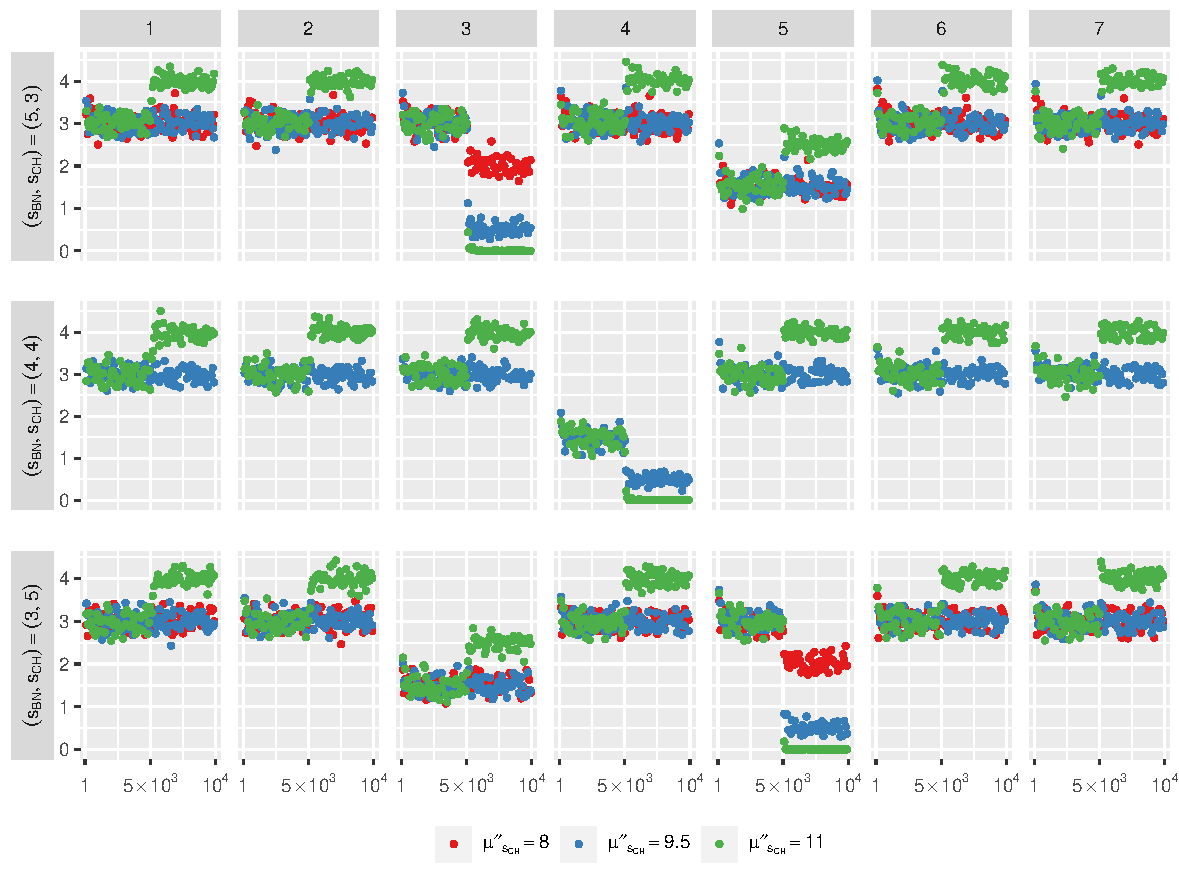
\includegraphics[width=1\textwidth]{ProcessingIncrease17_Blocking_time_MEAN_Starving_time_MEAN}
\caption[Value $I_s$ behavior with different processing time increase levels]{Value $I_s$ considering three different mean processing time increase levels $\mu_{s_{CH}}''$ and three bottleneck - changing stage configurations $(s_{BN},s_{CH})$. Models with $cl_s=6$.}
\label{fig:Value $I_s$ behavior with different processing time increase levels}
\end{figure}
Figure \ref{fig:Value $I_s$ behavior with different processing time increase levels} is helpful to understand how $I_s$ behaves.
\begin{itemize}
\item If a production capacity variation occurs, but the system remains stable, average $I_s$ changes only in correspondence of the changing stage $s_{CH}$ (it reduces if $\mu_{s_{CH}}''>\mu_{s_{CH}}'$, increases if $\mu_{s_{CH}}''<\mu_{s_{CH}}'$). \\It is visible in models with $\mu_{s_{CH}}''=8$ or $\mu_{s_{CH}}''=9.5$.
\item If a production capacity variation occurs and the system becomes unstable, average $I_s$ drops to $0$ in correspondence with the changing stage $s_{CH}$, and grows in all other stages. \\It is visible in models with $\mu_{s_{CH}}''=11$.
\end{itemize}
Since $I_s$ is also the sum of average Blocking\_time and average Starving\_time, this means that the sum of these KPIs, if the system remains stable, is constant in all stages except for the changing stage $s_{CH}$. Instead, if the system becomes unstable, the sum reduces to $0$ in $s_{CH}$ and grows in all other stages. At this point, it is interesting to visualize the relative proportions of Blocking\_time and Starving\_time in this sum. 
\begin{figure}[h] 
\centering
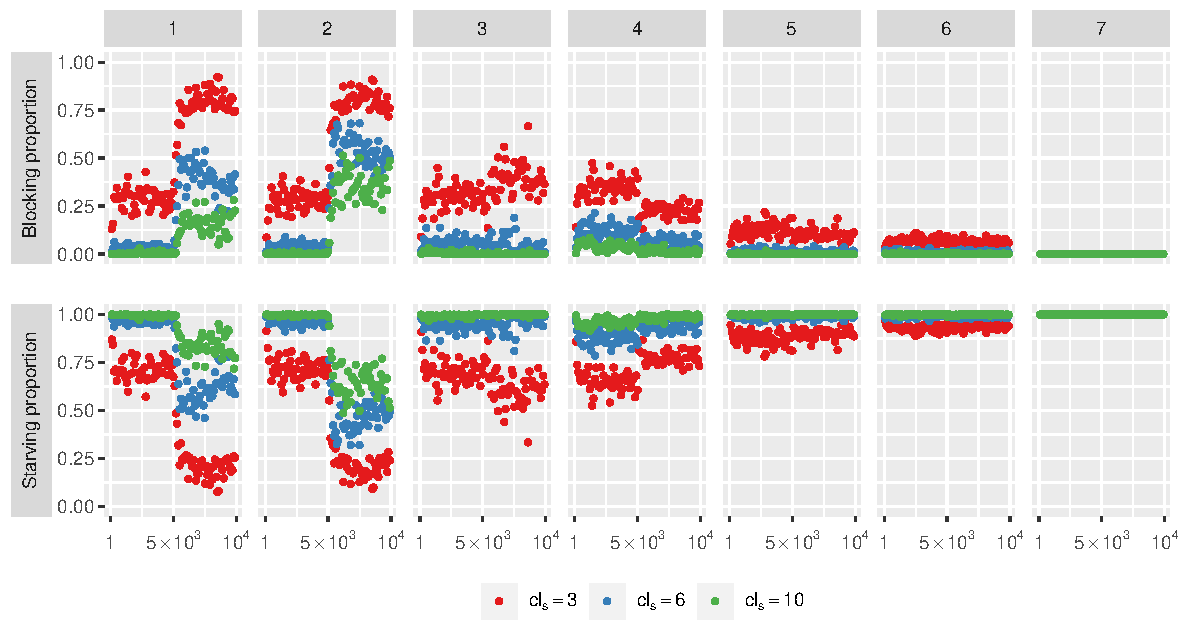
\includegraphics[width=1\textwidth]{ProcessingIncrease18_Blocking_prop_Starving_prop}
\caption[Average Blocking time and Starving time relative proportions considering different buffer capacity limits]{Average Blocking time and Starving time relative proportions considering different buffer capacity limits $cl_s$. Models with configurations $(s_{BN},s_{CH})=(5,3)$, and after-change mean processing time $\mu_{s_{CH}}''=9.5$.}
\label{fig:Average Blocking time and Starving time relative proportions considering different buffer capacity limits}
\end{figure}
Figure \ref{fig:Average Blocking time and Starving time relative proportions considering different buffer capacity limits} shows that 
\begin{itemize}
\item The contribution of average Blocking\_time in $I_s$ increases the smaller is the buffer.
\item The contribution of average Starving\_time in $I_s$ reduces the smaller is the buffer.
\end{itemize}
\subsubsection{Blocking\_prob and Starving\_prob KPIs}
Like Processing\_time, also Blocking\_time and Starving\_time can be represented in combination with Mid\_diff. The obtained KPIs are Blocking\_prob and Starving\_prob.
\begin{figure}[h] 
\centering
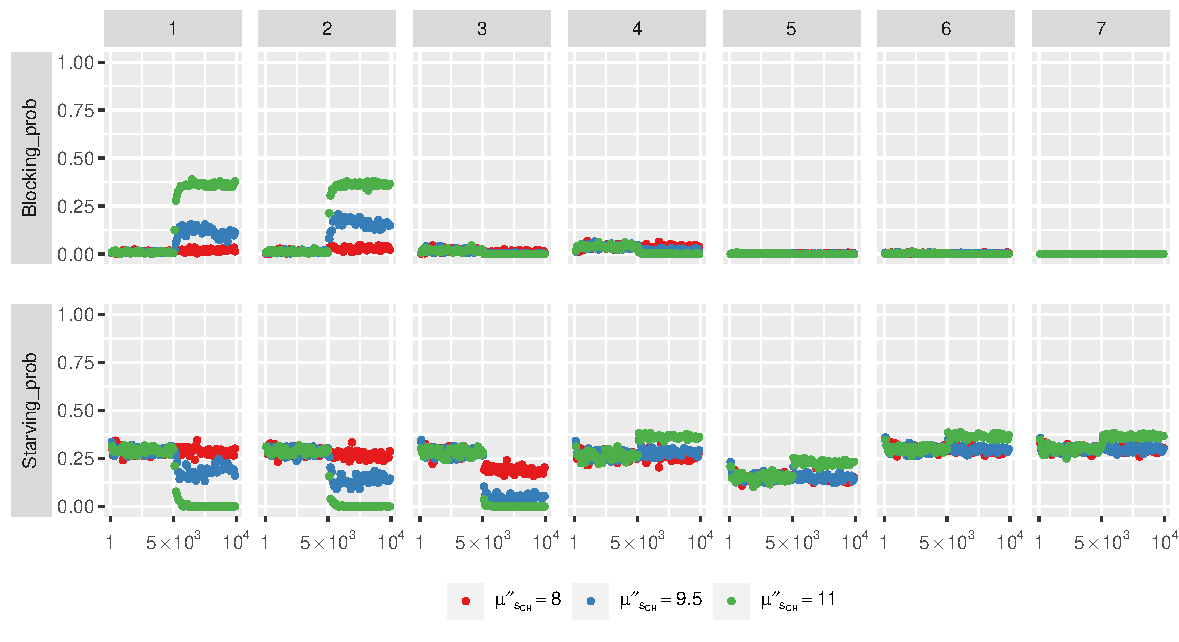
\includegraphics[width=1\textwidth]{ProcessingIncrease10_Blocking_prob_Starving_prob}
\caption[Blocking prob and Starving prob KPI behaviors with different processing time increase levels]{Blocking prob and Starving prob KPI behaviors considering three processing time increase levels $\mu_{s_{CH}}''$. Models with configurations $(s_{BN},s_{CH})=(5,3)$ and $cl_s=6$.}
\label{fig:Blocking prob and Starving prob KPIs behavior with different processing time increase levels}
\end{figure}
Figure \ref{fig:Blocking prob and Starving prob KPIs behavior with different processing time increase levels} portrays an example of these KPIs. These KPIs indicate how much of the available time was spent by the resources without being utilized. The observations that can be made regarding these KPI behaviors are analogous to one done for Blocking\_time and Starving\_time. 
\newpage
\subsection{Waiting\_time and Average\_Queue KPIs}
\label{Waiting time and Average Queue KPIs - Processing time variation}
Blocking\_time and Starving\_time help to monitor the effects of a variation on the exploitation of resources in stages different from the changing stage; indirectly, these KPIs allow to get insights about the buffer saturation levels. However, to get a closer and more precise view of job queues statuses, it is necessary to resort to Waiting\_time KPI. In this subsection, firstly Waiting\_time and Average\_Queue, which is its derived Stage State KPI, behaviors are discussed; then, at the end, the effects of having an unlimited buffer in the first stage are briefly addressed.
\subsubsection{Processing time increase effects on Waiting\_time KPI}
\begin{figure}[h] 
\centering
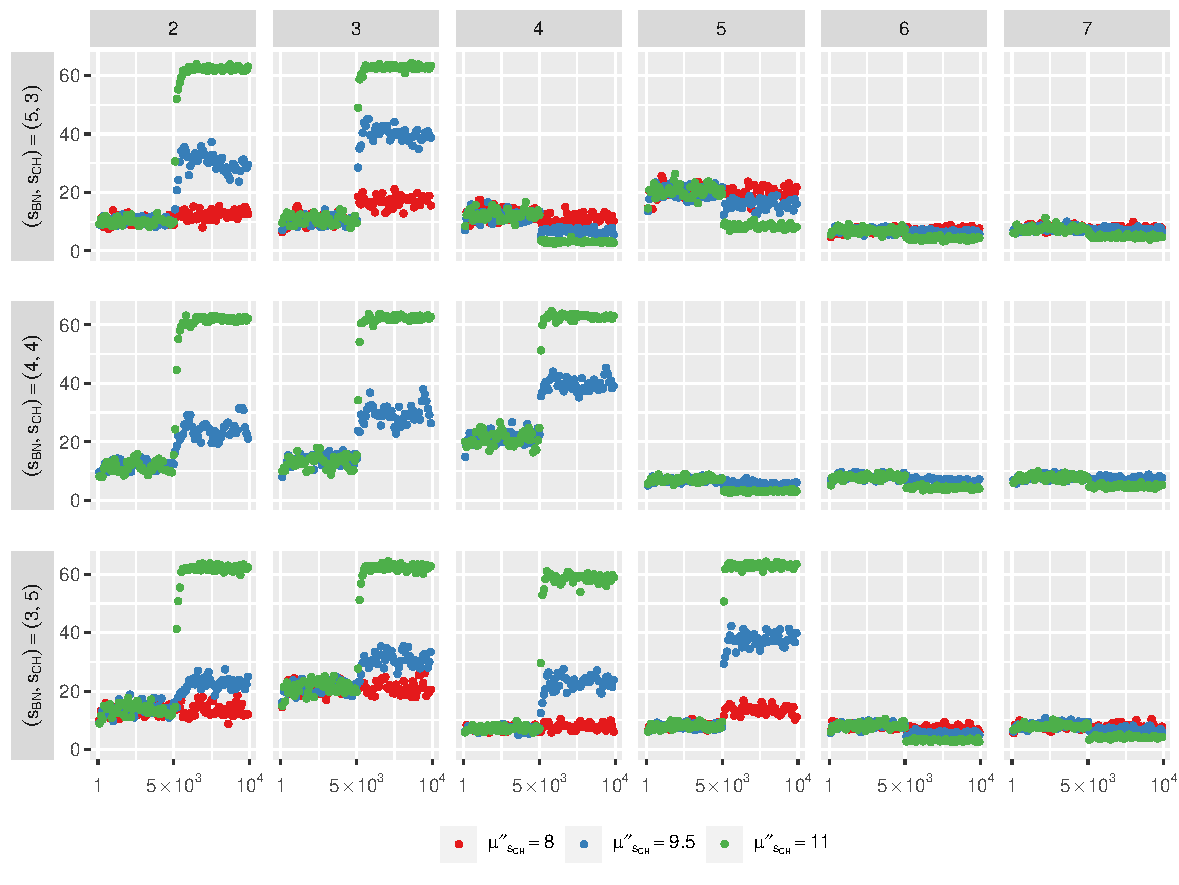
\includegraphics[width=1\textwidth]{ProcessingIncrease12_Waiting_time_MEAN}
\caption[Waiting time RW KPI behavior with different processing time increase levels]{Waiting time RW KPI behavior considering three processing time increase levels $\mu_{s_{CH}}''$ and three bottleneck - changing stage configurations $(s_{BN},s_{CH})$. Models with $cl_s=6$.}
\label{fig:Waiting time KPI behavior with different processing time increase levels}
\end{figure}
Figure \ref{fig:Waiting time KPI behavior with different processing time increase levels} the behavior of Waiting\_time\_MEAN RW KPI in case of a production capacity decrease in a stage. 
\begin{itemize}
\item If a resource loses production capacity to the point that the system becomes unstable:
\begin{itemize}
\item In stages upstream the changing stage $s_{CH}$, average Waiting\_time increases and settles around value $LW_s$.
\item In correspondence of the changing stage $s_{CH}$, average Waiting\_time increases and settles around value $LW_s$.
\item In stages downstream the changing stage $s_{CH}$, average Waiting\_time decreases towards $0$.
\end{itemize}
This is visible in models with any configuration $(s_{BN},s_{CH})$ having after-change mean processing time value $\mu_{s_{CH}}''=11$.\\
$LW_s$ is equal to the product of average Input\_diff and the maximum buffer capacity of stage $s$, $cl_s$. In other words, it is a limit that depends on the cycle time as seen in stage $s$, and on stage $s$ buffer capacity. 
\item If a resource loses production capacity but the system remains stable:
\begin{itemize}
\item In stages upstream the changing stage $s_{CH}$, average Waiting\_time increases.
\item In correspondence of the changing stage $s_{CH}$, average Waiting\_time increases.
\item In stages downstream the changing stage $s_{CH}$, average Waiting\_time decreases.
\end{itemize}
This is visible in models with any configuration $(s_{BN},s_{CH})$ having after-change mean processing time value $\mu_{s_{CH}}''=8$ or $\mu_{s_{CH}}''=9.5$.
\item Average Waiting\_time variations are wider the more significant is the increase of processing time.
\item Average Waiting\_time variations in a certain stage $s$ are less and less relevant the further stage $s$ is from the changing stage $s_{CH}$, both upstream and downstream $s_{CH}$. 
\item Average Waiting\_time of stage $s$ stabilizes around the average time a job has to wait in stage $s$ buffer before seizing the resource. \\This is visible in all models, before and after the variation occurring when Case ID reaches value $5000$.
\end{itemize}
Average Waiting\_time of stage $s$ follows the theoretical behavior of the average time a job spends in stage $s$ buffer. Indeed, the time a job has to wait is longer in stages upstream and in correspondence with the bottleneck and lower in stages downstream. Moreover, if the system becomes unstable, buffers in stages upstream and in correspondence with the bottleneck get saturated, and the job queue is longer the higher the buffer capacity limit is. Since jobs in buffers, before seizing the resource, have to wait until all other jobs which have entered before them are processed\footnote{The service policy was assumed to be FIFO, see section \ref{Considered systems}}, the time they have to wait is equal to the number of jobs in the queue before them (which is equal to the buffer limit, since it is full) multiplied by the job inter-arrival time in the queue, that is the cycle time.
\subsubsection{Value $LW_s$ and Average\_Queue KPI}
$LW_s$ has been defined as a limit value for stage $s$ average Waiting\_time if the system becomes unstable, however its equation can be generalized to be also valid when the system works in a stable condition. Indeed, theory says that the job average waiting time in a queue is always equal to the average cycle time multiplied by the average number of jobs in the queue. This means that average Waiting\_time of stage $s$ is always equal to the product of stage $s$ average Input\_diff\footnote{Input\_diff is the indicator of the cycle time as it is seen at buffer entrances} and the average number of jobs in stage $s$ buffer. $LW_s$ is just the value taken by average Waiting\_time in stages upstream the bottleneck when a particular situation occurs, that is when system becomes unstable. \\
This observation explains why Average\_queue (i.e. the ratio between average Waiting\_time and Input\_diff, see subsection \ref{Derived KPIs}) indicates the average number of jobs in a buffer.
\begin{figure}[h] 
\centering
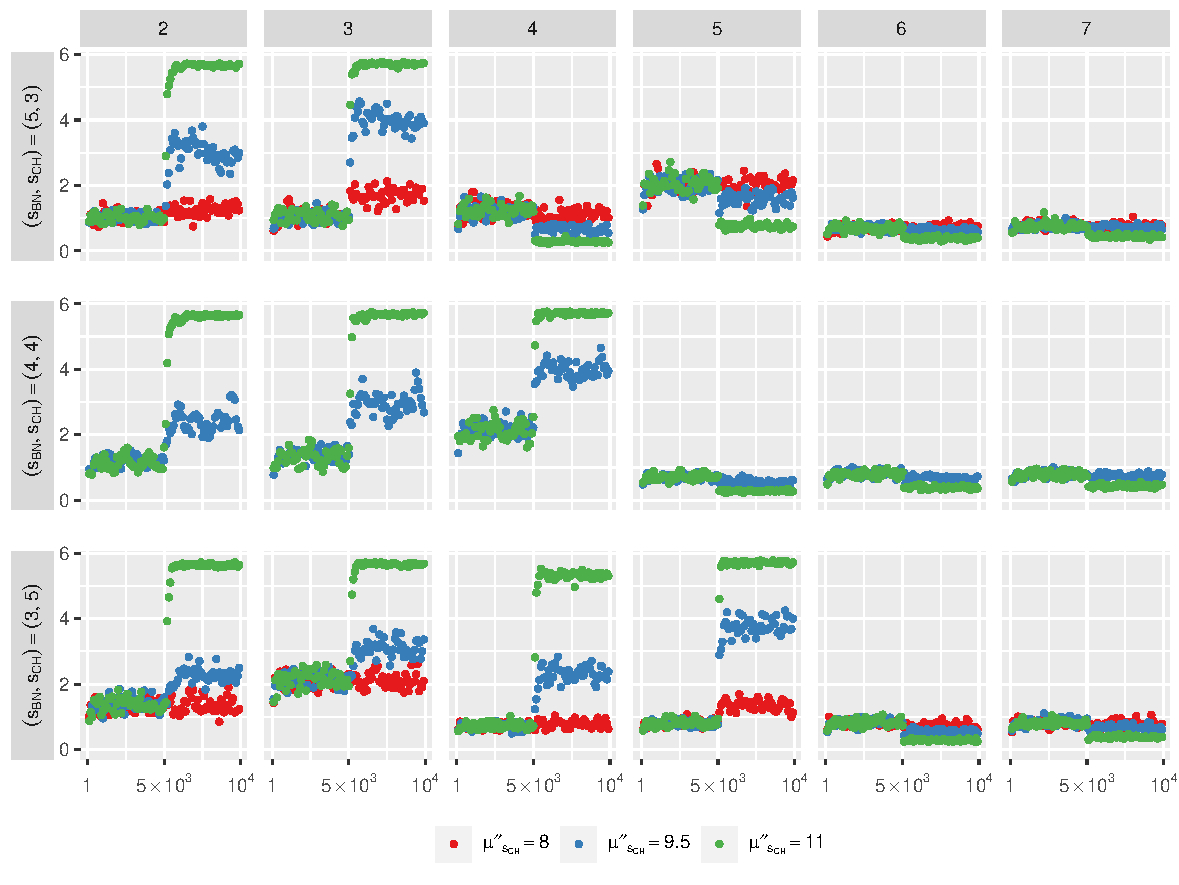
\includegraphics[width=1\textwidth]{ProcessingIncrease13_Average_Queue}
\caption[Average Queue KPI behavior with different processing time increase levels]{Average Queue KPI behavior considering three processing time increase levels $\mu_{s_{CH}}''$ and three bottleneck - changing stage configurations $(s_{BN},s_{CH})$. Models with $cl_s=6$.}
\label{fig:Average Queue KPI behavior with different processing time increase levels}
\end{figure}
Figure \ref{fig:Average Queue KPI behavior with different processing time increase levels} portrays Average\_Queue considering the same models of figure \ref{fig:Waiting time KPI behavior with different processing time increase levels}. This KPI behavior is similar to the Waiting\_time one 
\begin{itemize}
\item If a resource loses production capacity to the point that the system becomes unstable:
\begin{itemize}
\item In stages upstream the changing stage $s_{CH}$, Average\_Queue increases and settles around the buffer capacity limit $cl_s$.
\item In correspondence of the changing stage $s_{CH}$, Average\_Queue increases and settles around the buffer capacity limit $cl_{s_{CH}}$.
\item In stages downstream the changing stage $s_{CH}$, Average\_Queue decreases towards $0$.
\end{itemize}
This is visible in models with any configuration $(s_{BN},s_{CH})$ having after-change mean processing time value $\mu_{s_{CH}}''=11$.
\item If a resource loses production capacity but the system remains stable:
\begin{itemize}
\item In stages upstream the changing stage $s_{CH}$, Average\_Queue increases towards the buffer capacity limit $cl_s$.
\item In correspondence of the changing stage $s_{CH}$, Average\_Queue increases towards the buffer capacity limit $cl_{s_{CH}}$.
\item In stages downstream the changing stage $s_{CH}$, Average\_Queue decreases towards $0$.
\end{itemize}
This is visible in models with any configuration $(s_{BN},s_{CH})$ having after-change mean processing time value $\mu_{s_{CH}}''=8$ or $\mu_{s_{CH}}''=9.5$.
\item Average\_Queue variations are wider the more significant is the decrease of processing time.
\item Average\_Queue variations in a certain stage $s$ are less and less relevant the further stage $s$ is from the changing stage $s_{CH}$, both upstream and downstream. 
\item Average\_Queue of stage $s$ stabilizes around the average number of jobs present in stage $s$ buffer. \\This is visible in all models, before and after the variation occurring when Case ID reaches value $5000$.
\end{itemize}
\subsubsection{Waiting\_time behavior considering different buffer sizes}
As said before, Waiting\_time and Average\_Queue behaviors depend on buffer capacity limits. However, the buffer limitation does not affect these KPIs only when the system is unstable (i.e. when Waiting\_time reaches its limit $LW_s$ and Average\_Queue settles around the buffer maximum capacity $cl_s$), but it can influence them also when the system is stable. For sake of brevity, since Waiting\_time and Average\_Queue behaviors are very similar, only plots of the first one are displayed.
\begin{figure}[h] 
\centering
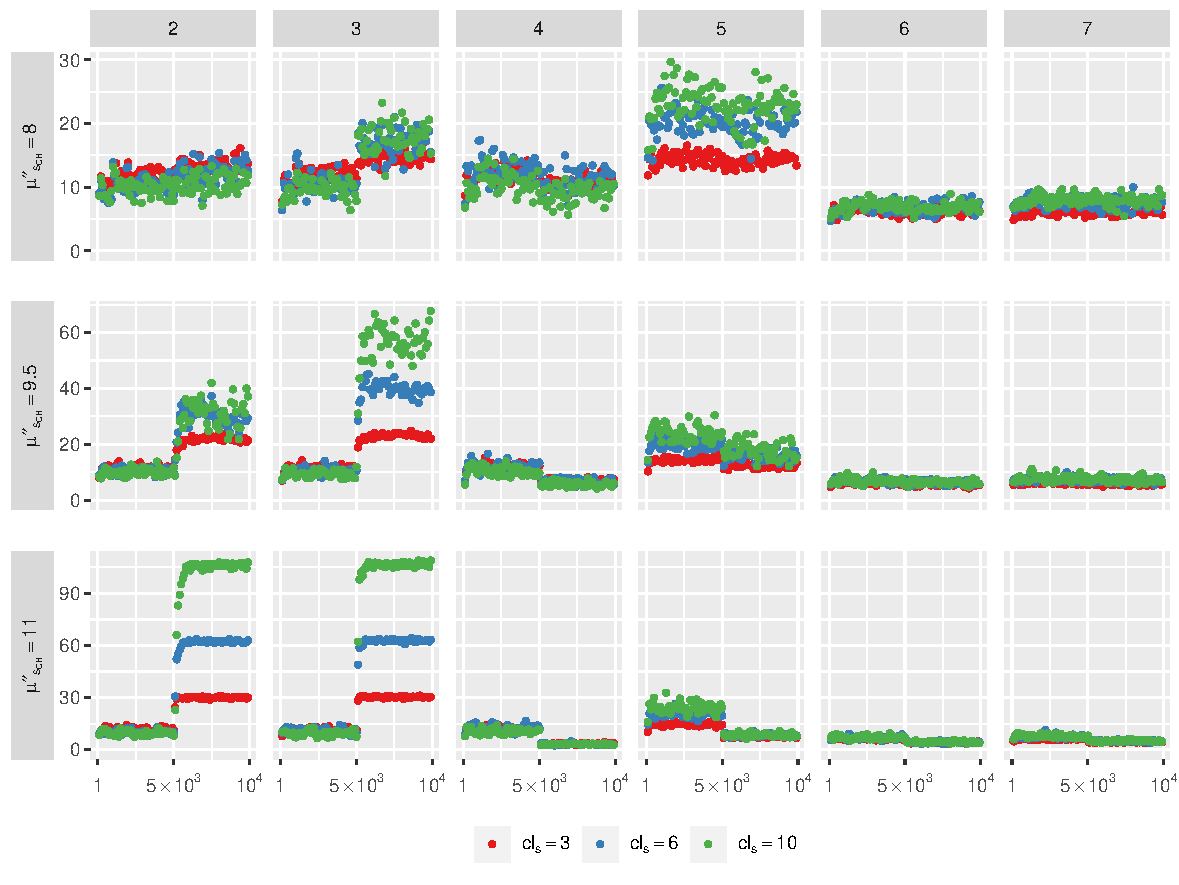
\includegraphics[width=1\textwidth]{ProcessingIncrease14_Waiting_time_MEAN}
\caption[Average Waiting time KPI behavior with different processing time increase levels considering different buffer capacity limits]{Average Waiting time KPI behavior considering three different mean processing time increase levels $\mu_{s_{CH}}$ and three buffer capacity limits $cl_s$. Models with configuration $(s_{BN},s_{CH})=(5,3)$.}
\label{fig:Average Waiting time KPI behavior with different processing time increase levels considering different buffer capacity limits}
\end{figure}
Figure \ref{fig:Average Waiting time KPI behavior with different processing time increase levels considering different buffer capacity limits} shows Waiting\_time in case of production capacity loss, considering three different buffer limits $cl_s$. Since the influence of buffer capacity limits on Waiting\_time and Average\_Queue behaviors is quite complex and an in-depth analysis falls outside the goal of this thesis, the observations here listed are always valid but insufficient to fully describe this dependence.
\begin{itemize}
\item When a resource loses production capacity, the higher the capacity limit $cl_s$ is, the wider the increase of average Waiting\_time in correspondence of the changing stage $s_{CH}$. \\This is visible in correspondence with the changing stage $s_{CH}=3$, comparing models with different buffer capacity limits $cl_s$.
\item When a resource loses production capacity but the system remains stable, the higher the capacity limit $cl_s$ is, the less relevant the spread of average Waiting\_time variation is in stages upstream and downstream the changing stage $cl_s$. \\This is visible upstream and downstream the changing stage $s_{CH}=3$, comparing models with different buffer capacity limits $cl_s$, having after-change mean processing time value $\mu_{s_{CH}}''=8$ or $\mu_{s_{CH}}''=9.5$.
\end{itemize}
To observe another impact of buffer capacity limits on Waiting\_time, systems with unlimited buffer are briefly considered. Indeed, even if it is not a realistic condition, it can be interpreted as a case of systems having buffers with extremely high capacity limits. 
\begin{figure}[h] 
\centering
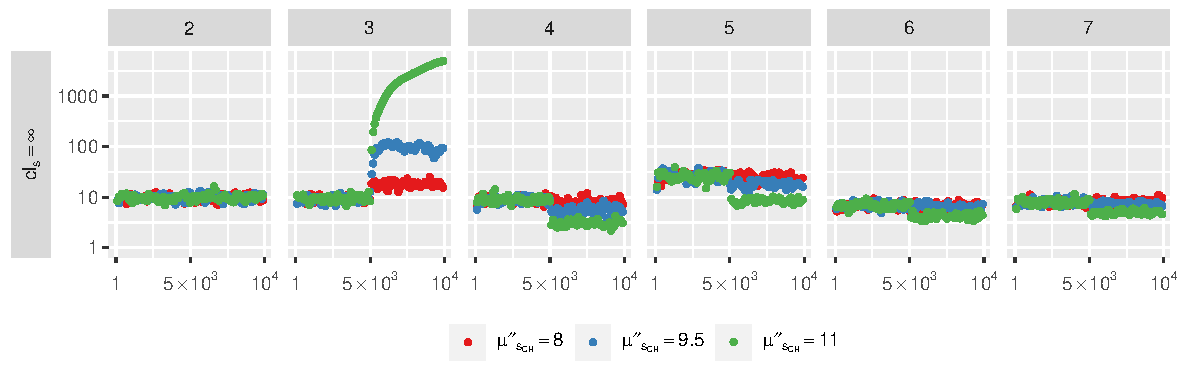
\includegraphics[width=1\textwidth]{ProcessingIncrease19_Waiting_time_MEAN}
\caption[Average Waiting time KPI behavior with different processing time increase levels considering buffers with unlimited capacity]{Average Waiting time KPI behavior considering three different mean processing time increase levels $\mu_{s_{CH}}$ and buffers with unlimited capacity. Models with configuration $(s_{BN},s_{CH})=(5,3)$ and $cl_s=\infty$. Graphs with log-scale on y-axis.}
\label{fig:Average Waiting time KPI behavior with different processing time increase levels considering buffers with unlimited capacity}
\end{figure}
Figure \ref{fig:Average Waiting time KPI behavior with different processing time increase levels considering buffers with unlimited capacity} shows average Waiting\_time behavior in case of a production capacity decrease when all buffers have unlimited capacity. The effects of high capacity buffers are taken to the extreme: when the changing stage $s_{CH}$ processing time increases, average Waiting\_time extensively decreases in stages downstream $s_{CH}$ and increases in correspondence with the changing stage $s_{CH}$. If, after the variation, the system becomes unstable (as in model with $\mu_{s_{CH}}''=11$), average Waiting\_time of stage $s_{CH}$ even grows towards infinity, since buffers have no boundaries and job mean inter-arrival in the first stage is lower than the mean processing time of the changing stage ($\mu_a<\mu_{s_{CH}}''$). However, it can be noticed that Waiting\_time does not change in stage $s=2$, upstream $s_{CH}$, even when the system becomes unstable. 
\\ The discussion about this particular (not realistic) case was included to show that buffers having high capacity limits work as temporary decoupling points, delaying variation effects on KPIs to spread upstream the stage in which they are positioned. The delay caused by infinite buffers (which are permanent decoupling points) is infinite, and so KPIs upstream never change.
\subsubsection{Processing time decrease effects on Waiting\_time and Average\_Queue KPIs}
The effects of a production capacity increase on Waiting\_time and Average\_Queue KPIs are the opposite than the ones caused by a production capacity decrease.
\begin{figure}[h] 
\centering
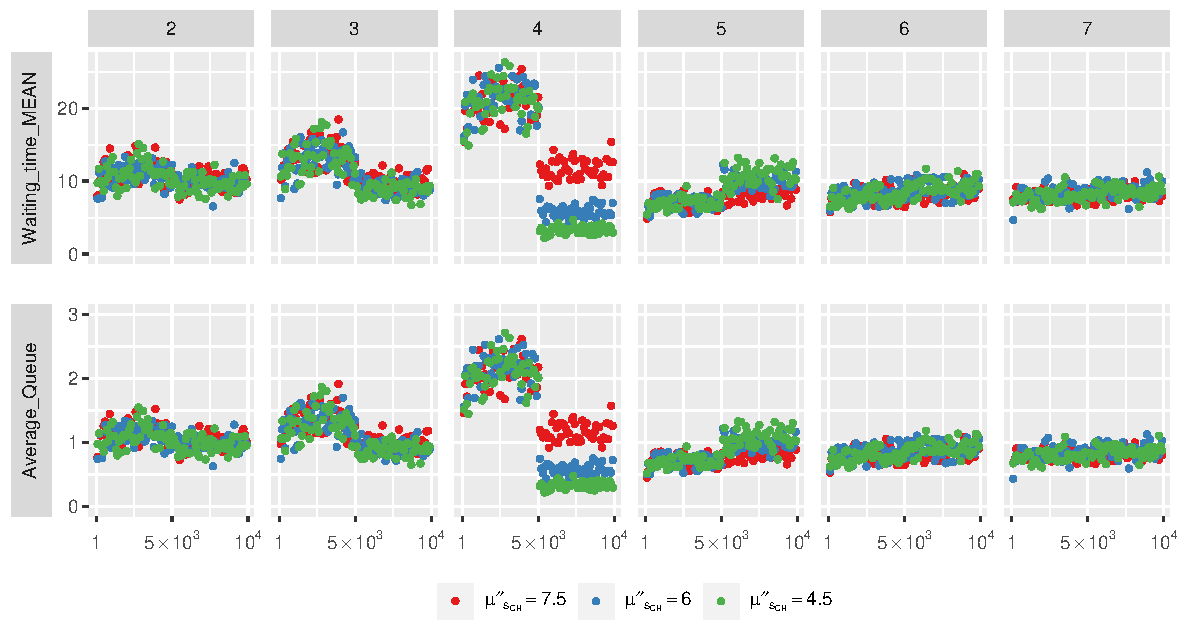
\includegraphics[width=1\textwidth]{ProcessingIncrease15_Waiting_time_MEAN_Average_Queue}
\caption[Waiting time RW and Average Queue KPIs behaviors with different processing time decrease levels]{Waiting time RW and Average Queue KPIs behaviors considering different processing time decrease levels $\mu_{s_{CH}}''$. Models with configuration $(s_{BN},s_{CH})=(4,4)$ and $cl_s=6$.}
\label{fig:Waiting time RW and Average Queue KPIs behaviors with different processing time decrease levels}
\end{figure}
Figure \ref{fig:Waiting time RW and Average Queue KPIs behaviors with different processing time decrease levels} shows Waiting\_time and Average\_Queue behaviors in case of a mean processing time $\mu_{s_{CH}}$ decrease. 
\begin{itemize}
\item If a resource increases its production capacity 
\begin{itemize}
\item In stages upstream the changing stage $s_{CH}$, average Waiting\_time and Average\_Queue decrease.
\item In correspondence of the changing stage $s_{CH}$, average Waiting\_time and Average\_Queue decrease.
\item In stages downstream the changing stage $s_{CH}$, average Waiting\_time and Average\_Queue increase.
\end{itemize}
\item Average Waiting\_time and Average\_Queue variations are wider the more significant is the increase of processing time.
\item Average Waiting\_time and Average\_Queue variations in a certain stage $s$ are less and less relevant the further stage $s$ is from the changing stage $s_{CH}$, both upstream and downstream. 
\end{itemize}
\subsubsection{Waiting\_time and Average\_Queue KPI behaviors in the first stage of the line}
It should be noted that the first stage has not been included in any figure of this subsection. As a matter of fact, since the first stage buffer is unlimited, the information of how much time jobs spend in it and how many are present at the same time is not useful. Moreover, Waiting\_time and Average\_Queue of the first stage infinitely grow when the system becomes unstable, a circumstance in which Average\_Queue even becomes a wrong indicator of the average number of jobs in the buffer.
\begin{figure}[h] 
\centering
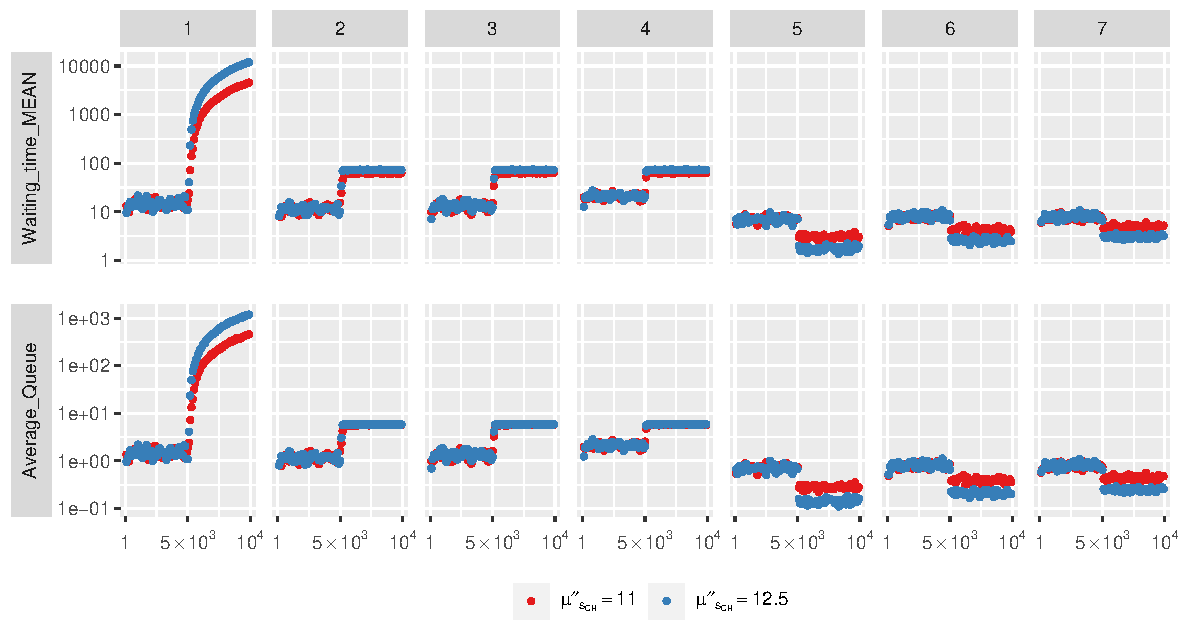
\includegraphics[width=1\textwidth]{ProcessingIncrease16_Waiting_time_MEAN_Average_Queue}
\caption[Waiting time RW and Average Queue KPIs behaviors with different processing time increase levels that make the system unstable]{Waiting time RW and Average Queue KPIs behaviors considering different processing time increase levels that make the system unstable. Models with configuration $(s_{BN},s_{CH})=(4,4)$ and $cl_s=6$. Graphs with log-scale on y-axis.}
\label{fig:Waiting time RW and Average Queue KPIs behaviors with different processing time increase levels that make the system unstable}
\end{figure}
Figure \ref{fig:Waiting time RW and Average Queue KPIs behaviors with different processing time increase levels that make the system unstable} shows the behaviors of Waiting\_time and Average\_Queue when the system becomes unstable: in the first stage both these KPIs increase towards infinity. In particular it should be noticed that, at the end of the process, but Average\_Queue grows as if new jobs kept arriving, even if no more jobs enter the line and the buffer starts emptying. This error verifies because in this situation Waiting\_time (rightly) keeps increasing, yet Input\_diff remains equal to the bottleneck processing time. Reminding how Average\_Queue is computed, this means that the numerator keeps growing while the denominator is fixed, making the KPI erroneously continuously increasing. \\Because of these irregular behaviors, first stage plots have been omitted in previous figures. 
\newpage
\section{Buffer capacity variation}
A buffer capacity variation does not have effects on resource processing time and, so, never influences the system cycle time. Therefore, this type of variation is visible only in KPIs related to buffers (i.e. Waiting\_time, Blocking\_time and Starving\_time, and the relative Stage State KPIs), while the others (CCI KPIs, Processing\_time and Utilization) are not subject to any change. Plots of KPIs not influenced by buffer capacity variations are not shown and discussed, to restrain the analysis to the most relevant indicators.
\subsection{Waiting\_time KPI}
\label{Waiting time KPI - Buffer capacity variation}
Waiting\_time and Average\_Queue are strongly influenced by buffer capacity limits (as shown in subsection \ref{Waiting time and Average Queue KPIs - Processing time variation}) and are directly related to queue statuses. In this subsection Waiting\_time behavior is analyzed in situations where a buffer capacity variation verifies, while Average\_Queue is not discussed, since it shows the same behavior of Waiting\_time. At the end of the subsection the problem of buffers having high capacity limits before the capacity variation is presented.
\subsubsection{Buffer capacity increase effects on Waiting\_time KPI}
\begin{figure}[h] 
\centering
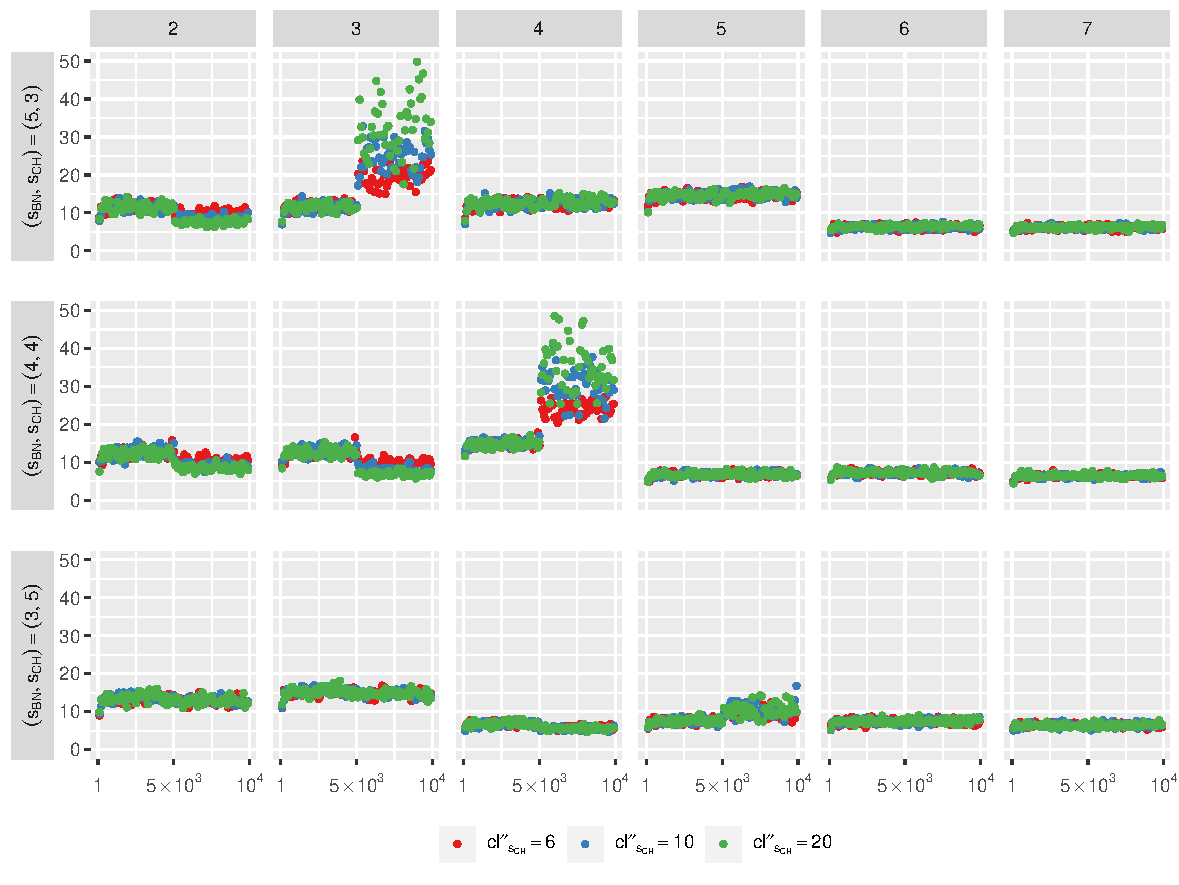
\includegraphics[width=1\textwidth]{BufferIncrease1_Waiting_time_MEAN}
\caption[Waiting time RW KPI behavior with different buffer capacity increase levels]{Waiting time RW KPI behavior considering different buffer capacity increase levels $cl_{s_{CH}}''$ and three bottleneck - changing stage configurations $(s_{BN},s_{CH})$. Models with $cl_s'=3$.}
\label{fig:Waiting time RW KPI behavior with different buffer capacity increase levels}
\end{figure}
Figure \ref{fig:Waiting time RW KPI behavior with different buffer capacity increase levels} shows average Waiting\_time behavior when a buffer capacity increases.
\begin{itemize}
\item If a buffer capacity increases
\begin{itemize}
\item In stages upstream the changing stage $s_{CH}$, average Waiting\_time decreases.
\item In correspondence of the changing stage $s_{CH}$, average Waiting\_time increases.
\item In stages downstream the changing stage $s_{CH}$, average Waiting\_time does not significantly change.
\end{itemize}
\item Average Waiting\_time variations are wider the larger the increase of buffer capacity is. \\This is visible comparing models with different after-change buffer capacities $cl_{s_{CH}}''$. 
\item Average Waiting\_time variations are 
\begin{itemize}
\item wider if the changing stage is upstream or in correspondence with the bottleneck ($s_{CH} \leqslant s_{BN}$)
\item narrower if the changing stage is downstream the bottleneck ($s_{CH}>s_{BN}$)
\end{itemize}
This is visible comparing models having bottleneck-changing stage configurations $(s_{BN},s_{CH})=(5,3)$ (changing stage upstream the bottleneck) or $(s_{BN},s_{CH})=(4,4)$ (changing stage in correspondence with the bottleneck) with models having $(s_{BN},s_{CH})=(3,5)$ (changing stage downstream the bottleneck) . 
\item Average Waiting\_time variations in a certain stage $s$ are less and less relevant the further stage $s$ is from the changing stage $s_{CH}$, both upstream and downstream $s_{CH}$. 
\end{itemize}
\subsubsection{Waiting\_time behavior considering different initial buffer sizes $cl_s'$}
In certain conditions, buffer capacity variations may have no effects on Waiting\_time. The occurrence of a change of this KPI mainly relies on the initial buffer saturation levels before the capacity variation verifies. 
\begin{figure}[h] 
\centering
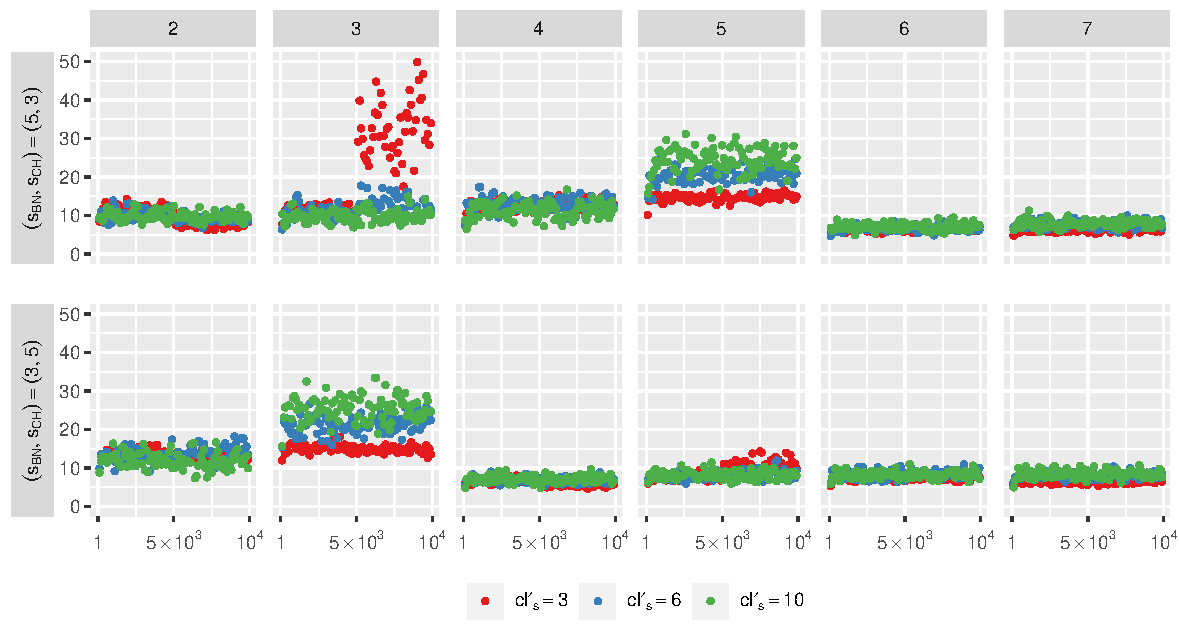
\includegraphics[width=1\textwidth]{BufferIncrease2_Waiting_time_MEAN}
\caption[Waiting time RW KPI behavior with different initial buffer capacity levels]{Waiting time RW KPI behavior considering different initial buffer capacity levels $cl_s'$ and two bottleneck-changing stage configurations $(s_{BN},s_{CH})$. Models with $cl_s''=20$.}
\label{fig:Waiting time RW KPI behavior with different initial buffer capacity levels}
\end{figure}
Figure \ref{fig:Waiting time RW KPI behavior with different initial buffer capacity levels} shows average Waiting\_time behavior considering different initial buffer capacities $cl_s'$. \\When a capacity limit increases:
\begin{itemize}
\item If buffers tend to be saturated, average Waiting\_time significantly changes. \\This is visible in models with before-change buffer capacity $cl_s'=3$, in particular in correspondence with the changing stage $s_{CH}$.
\item If buffers tend to be unsaturated, average Waiting\_time does not change. \\This is visible in models with before-change buffer capacity $cl_s'=10$.
\item If buffers are on average halfway saturated, average Waiting\_time behavior mostly depends on the position of the changing stage with respect to the bottleneck. \\This is visible in models with before-change buffer capacity $cl_s'=6$: when $s_{CH}$ is upstream $s_{BN}$ (i.e. model with configuration $(s_{BN},s_{CH})=(5,3)$), average Waiting\_time (slightly) changes in correspondence of $s_{CH}$.\footnote{This also verifies when the variation occurs in correspondence with the changing stage $s_{CH}$} When $s_{CH}$ is downstream $s_{BN}$ (i.e. model with configuration $(s_{BN},s_{CH})=(3,5)$), average Waiting\_time does not significantly change of $s_{CH}$
\end{itemize}
\subsubsection{Buffer capacity decrease effects on Waiting\_time KPI}
\begin{figure}[h]
\centering
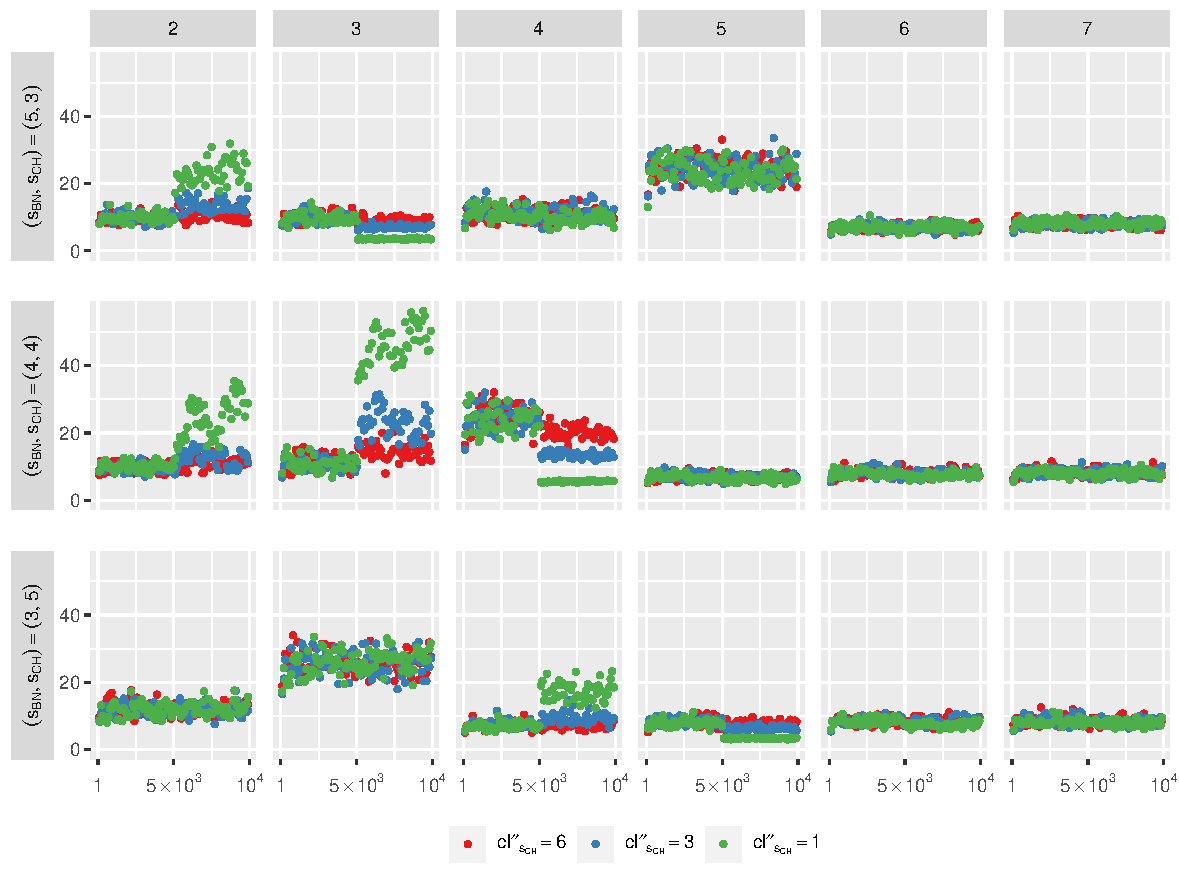
\includegraphics[width=1\textwidth]{BufferIncrease3_Waiting_time_MEAN}
\caption[Waiting time RW KPI behavior with different buffer capacity decrease levels]{Waiting time RW KPI behavior considering different buffer capacity decrease levels  $cl_s''$. Models with $cl_s'=10$)}
\label{fig:Waiting time RW KPI behavior with different buffer capacity decrease levels}
\end{figure}
Figure \ref{fig:Waiting time RW KPI behavior with different buffer capacity decrease levels} shows average Waiting\_time behavior when a buffer capacity decreases.
\begin{itemize}
\item If a buffer capacity reduces 
\begin{itemize}
\item In stages upstream the changing stage $s_{CH}$, average Waiting\_time increases.
\item In correspondence of the changing stage $s_{CH}$, average Waiting\_time decreases.
\item In stages downstream the changing stage $s_{CH}$, average Waiting\_time does not significantly change.
\end{itemize}
\item Average Waiting\_time variations are wider the larger the decrease of buffer capacity is. \\This is visible comparing models with different after-change buffer capacities $cl_{s_{CH}}''$. 
\item Average Waiting\_time variations are 
\begin{itemize}
\item wider if the changing stage is upstream or in correspondence with the bottleneck ($s_{CH} \leqslant s_{BN}$)
\item narrower if the changing stage is downstream the bottleneck ($s_{CH}>s_{BN}$)
\end{itemize}
This is visible comparing models having bottleneck-changing stage configurations $(s_{BN},s_{CH})=(5,3)$ (changing stage upstream the bottleneck) or $(s_{BN},s_{CH})=(4,4)$ (changing stage in correspondence with the bottleneck) with models having $(s_{BN},s_{CH})=(3,5)$ (changing stage downstream the bottleneck). 
\item Average Waiting\_time variations in a certain stage $s$ are less and less relevant the further stage $s$ is from the changing stage $s_{CH}$, both upstream and downstream. 
\end{itemize}
\subsubsection{Variation conceal caused by before-change high capacity buffers}
It is important to highlight that not every buffer capacity limit variation is detectable using Waiting\_time or Average\_Queue. Indeed, when before-change buffer sizes are much higher than necessary, and so underused and largely unsaturated during the process, buffer capacity growths or limited capacity reductions are impossible to notice. It verifies because, if queues in buffers are consistently much lower than the capacity limit, a variation of the limit will not have effects on the queue: in case of a capacity increase, the added room is not used, while in case of a capacity decrease (if not too large), the removed space was not used before the change and, so, jobs are not influenced by the change.
\begin{figure}[h]
\centering
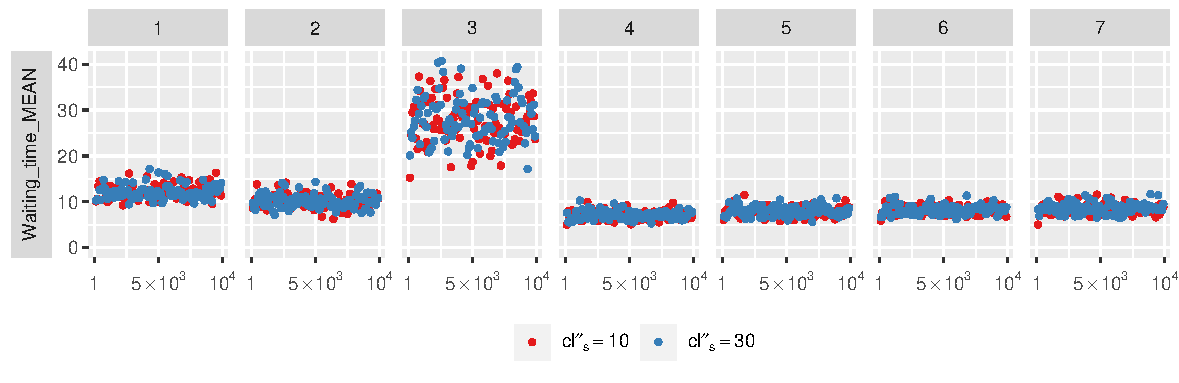
\includegraphics[width=1\textwidth]{BufferIncrease8_Waiting_time_MEAN}
\caption[Waiting time RW KPI behavior with different buffer capacity variation levels and high before-change buffer capacity limits]{Waiting time RW KPI behavior considering different buffer capacity variation levels $cl_s''$. Models with configuration $(s_{BN},s_{CH})=(3,5)$ and $cl_s'=20$.}
\label{fig:Waiting time RW KPI behavior with different buffer capacity variation levels and high before-change buffer capacity limits}
\end{figure}
Figure \ref{fig:Waiting time RW KPI behavior with different buffer capacity variation levels and high before-change buffer capacity limits} helps to visualize this kind of situation: all the buffers have high capacities ($cl_s'=20$), and so are extremely unsaturated. When the changing stage capacity limit increases to $cl_{s_{5}}=30$, average Waiting\_time behavior does not change. Moreover, since the changing stage is downstream the bottleneck ($s_{CH}=5>s_{BN}=3$), even a capacity limit decrease has no visible effects on average Waiting\_time.\\
Before-change high capacity buffers have also the same effects on Blocking\_time and Starving\_time KPIs, which are discussed in the next chapter. Therefore, it is possible to conclude that, if a buffer capacity change occurs in correspondence with a high capacity and extremely unsaturated buffer, it is not detectable with any KPI defined in this thesis. 
\newpage
\subsection{Blocking\_time and Starving\_time KPIs}
\label{Blocking time and Starving time KPIs - Buffer capacity variation}
Since Blocking\_time and Starving\_time KPI behaviors are specular (as seen in subsection \ref{Blocking time, Starving time and respective Stage State KPIs - Processing time variation}), they are analyzed together in this subsection. These KPI behaviors are influenced by both the production capacities of resources and the capacities of buffers. 
\subsubsection{Buffer capacity increase effects on Blocking\_time and Starving\_time KPIs}
\begin{figure}[h] 
\centering
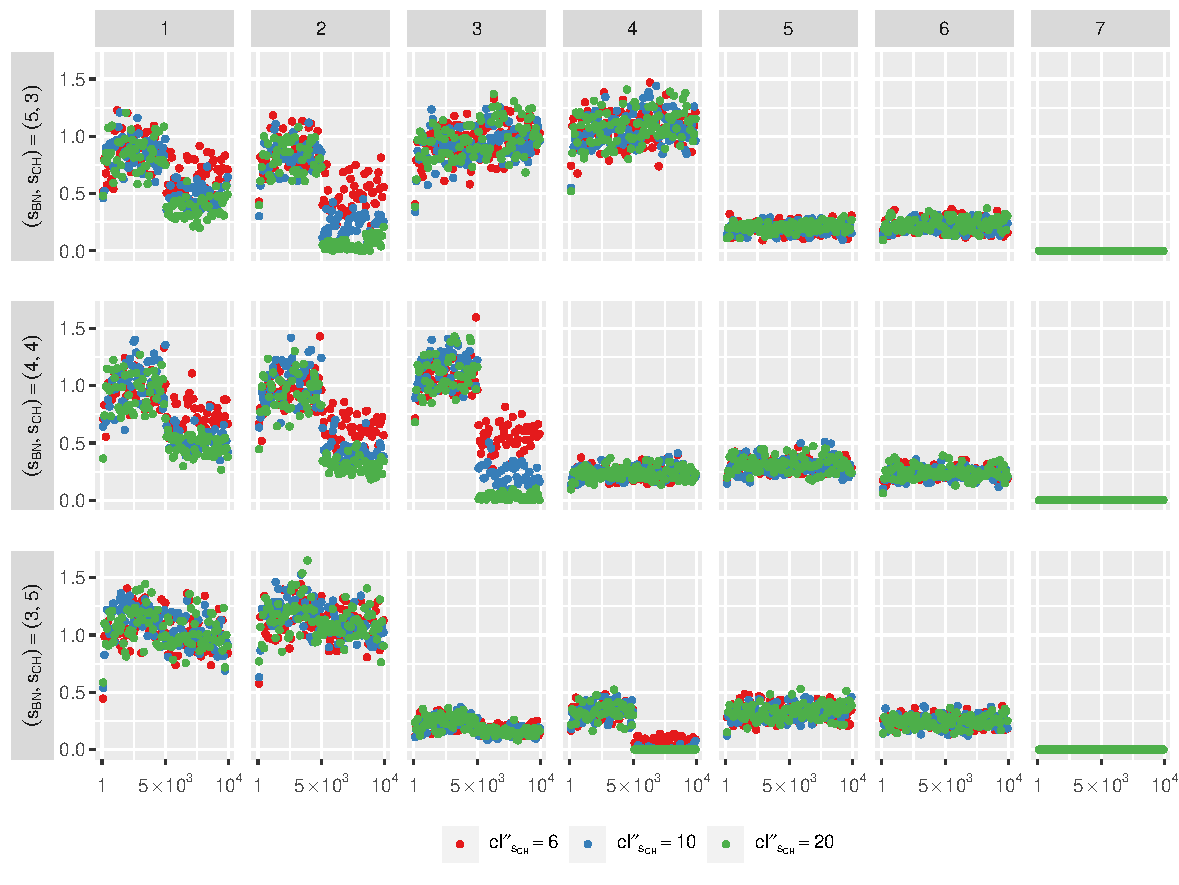
\includegraphics[width=1\textwidth]{BufferIncrease4_Blocking_time_MEAN}
\caption[Blocking time RW KPI behavior with different buffer capacity increase levels]{Blocking time RW KPI behavior considering different buffer capacity increase levels $cl_{s_{CH}}''$ and three bottleneck - changing stage configurations $(s_{BN},s_{CH})$. Models with $cl_s'=3$.}
\label{fig:Blocking time RW KPI behavior with different buffer capacity increase levels}
\end{figure}
\begin{figure}[h] 
\centering
\includegraphics[width=1\textwidth]{BufferIncrease5_Starving_time_MEAN}
\caption[Starving time RW KPI behavior with different buffer capacity decrease levels]{Starving time RW KPI behavior considering different buffer capacity increase levels $cl_{s_{CH}}''$ and three bottleneck - changing stage configurations $(s_{BN},s_{CH})$. Models with $cl_s'=3$.}
\label{fig:Starving time RW KPI behavior with different buffer capacity increase levels}
\end{figure}
Figure \ref{fig:Blocking time RW KPI behavior with different buffer capacity increase levels} and figure \ref{fig:Starving time RW KPI behavior with different buffer capacity increase levels} show, respectively, average Blocking\_time and average Starving\_time behaviors in case of buffer capacity increases. 
\begin{itemize}
\item If a buffer capacity increases
\begin{itemize}
\item In stages upstream the changing stage $s_{CH}$, average Blocking\_time decreases and average Starving\_time increases.
\item In correspondence of the changing stage $s_{CH}$, average Blocking\_time increases and average Starving\_time decreases.
\item In stages downstream the changing stage $s_{CH}$, both average Blocking\_time and average Starving\_time do not significantly change.
\end{itemize}
\item Average Blocking\_time and average Starving\_time variations are wider the larger the increase of buffer capacity is. \\This is visible comparing models with different after-change buffer capacities $cl_{s_{CH}}''$. 
\item Average Blocking\_time and average Starving\_time variations are 
\begin{itemize}
\item wider if the changing stage is upstream or in correspondence with the bottleneck ($s_{CH} \leqslant s_{BN}$)
\item narrower if the changing stage is downstream the bottleneck ($s_{CH}>s_{BN}$)
\end{itemize}
This is visible comparing models having bottleneck-changing stage configurations $(s_{BN},s_{CH})=(5,3)$ (changing stage upstream the bottleneck) or $(s_{BN},s_{CH})=(4,4)$ (changing stage in correspondence with the bottleneck) with models having $(s_{BN},s_{CH})=(3,5)$ (changing stage downstream the bottleneck) . 
\item Average Blocking\_time and average Starving\_time variations in a certain stage $s$ are less and less relevant the further stage $s$ is from the changing stage $s_{CH}$, both upstream and downstream $s_{CH}$. 
\end{itemize}
\subsubsection{Blocking\_time and Starving\_time behaviors considering different initial buffer sizes $cl_s'$}
As for Waiting\_time, buffer capacity variations may have no effects on Blocking\_time and Starving\_time. The occurrence of a change of these KPIs mainly rely on the initial buffer saturation levels before the capacity variation verifies. 
\begin{figure}[h] 
\centering
\includegraphics[width=1\textwidth]{BufferIncrease6_Blocking_time_MEAN_Starving_time_MEAN}
\caption[Blocking time and Starving time RW KPIs behaviors with different initial buffer capacity levels]{Blocking time and Starving time RW KPIs behaviors considering different initial buffer capacity levels $cl_s'$. Models with configuration $(s_{BN},s_{CH})=(5,3)$ and after-change value $cl_s''=20$.}
\label{fig:Blocking time and Starving time RW KPIs behaviors with different initial buffer capacity levels}
\end{figure}
Figure \ref{fig:Waiting time RW KPI behavior with different initial buffer capacity levels} shows average Blocking\_time and Starving\_time behaviors considering different initial buffer capacities $cl_s'$. \\When a capacity limit increases:
\begin{itemize}
\item If buffers tend to be saturated, average Blocking\_time and Starving\_time significantly change. \\This is visible in models with before-change buffer capacity $cl_s'=3$, in particular in correspondence with the changing stage $s_{CH}=3$.
\item If buffers tend to be unsaturated, average Blocking\_time and Starving\_time do not change. \\This is visible in models with before-change buffer capacity $cl_s'=10$.
\item If buffers are on average halfway saturated, average Blocking\_time and Starving\_time behaviors mostly depend on the position of the changing stage with respect to the bottleneck. \\This is visible in models with before-change buffer capacity $cl_s'=6$: when $s_{CH}$ is upstream $s_{BN}$ (i.e. model with configuration $(s_{BN},s_{CH})=(5,3)$), average Blocking\_time and Starving\_time (slightly) change in correspondence and upstream $s_{CH}$. When $s_{CH}$ is downstream $s_{BN}$ (i.e. model with configuration $(s_{BN},s_{CH})=(3,5)$), average Blocking\_time and Starving\_time do not significantly change.
\end{itemize}
\subsubsection{Buffer capacity decrease effects on Blocking\_time and Starving\_time}
\begin{figure}[h] 
\centering
\includegraphics[width=1\textwidth]{BufferIncrease7_Blocking_time_MEAN_Starving_time_MEAN}
\caption[Blocking time and Starving time RW KPIs behaviors with different buffer capacity decrease levels]{Blocking time and Starving time RW KPIs behaviors considering different buffer capacity decrease levels $cl_s''$. Models with configuration $(s_{BN},s_{CH})=(5,3)$ and $cl_s'=10$.}
\label{fig:Blocking time and Starving time RW KPIs behaviors with different buffer capacity decrease levels}
\end{figure}
Figure \ref{fig:Waiting time RW KPI behavior with different buffer capacity decrease levels} shows average Blocking\_time and Starving\_time behaviors when a buffer capacity decreases.
\begin{itemize}
\item If a buffer capacity reduces 
\begin{itemize}
\item In stages upstream the changing stage $s_{CH}$, average Blocking\_time increases and average Starving\_time decreases.
\item In correspondence of the changing stage $s_{CH}$, average Blocking\_time decreases and average Starving\_time increases.
\item In stages downstream the changing stage $s_{CH}$, both average Blocking\_time and average Starving\_time do not significantly change.
\end{itemize}
\item Average Blocking\_time and Starving\_time variations are wider the larger the decrease of buffer capacity is. \\This is visible comparing models with different after-change buffer capacities $cl_{s_{CH}}''$. 
\item Average  Blocking\_time and Starving\_time variations are 
\begin{itemize}
\item wider if the changing stage is upstream or in correspondence with the bottleneck ($s_{CH} \leqslant s_{BN}$)
\item narrower if the changing stage is downstream the bottleneck ($s_{CH}>s_{BN}$)
\end{itemize}
\item Average  Blocking\_time and Starving\_time variations in a certain stage $s$ are less and less relevant the further stage $s$ is from the changing stage $s_{CH}$, both upstream and downstream. 
\end{itemize}
\chapter{A map of variations}
\label{chapter 7}
\ifpdf
    \graphicspath{{Chapter7/Figs/}{Chapter7/Figs/PDF/}{Chapter7/Figs/}}
\else
    \graphicspath{{Chapter7/Figs/Vector/}{Chapter7/Figs/}}
\fi
This chapter provides a summary of variations, based on the results analyzed in chapter \ref{chapter 6}. The summary aims to fulfill the thesis goal outlined in section \ref{Aim of the work}, which is to define a map of variations to serve as a handbook that allows to interpret the indicator behaviors and relate a KPI change with a variation occurring in the real system. \\
The first section is dedicated to change detection, that is the step preliminary to the change identification (see introduction of chapter \ref{chapter 2}), in order to specify what system variation is possible to notice monitoring a certain KPI. \\In the second section, the process variation effects on each indicator is described and visualized through schemes representing abstractions of the KPI average behaviors, in order to outline if and how far they are fitting to give insights about the system variation extents. 
\section{Variation detection}
The goal of this section is to answer to two questions
\begin{center}
\textit{Which KPIs are able to detect a certain process variation?}\\
\vspace{3mm}
\textit{In what situation can a KPI detect a certain process variation?}
\end{center}
\begin{table}[H]
	\caption{Processing time variation detection}
	\centering
	\label{table: Processing time variation detection}
	\begin{tabular}{l c c c c l}
		\toprule
		\multirow{2}{*}{KPI} & & \multicolumn{2}{c}{Processing time} & & \multirow{2}{*}{Detection condition}\\ 
		\cmidrule(lr){3-4}
		& & Increase $\Uparrow$ & Decrease $\Downarrow$ \\
		\cmidrule{1-6}
		Input\_diff 		& & \checkmark & & & System becomes unstable \\
		Mid\_diff 			& & \checkmark & & & System becomes unstable \\
		Output\_diff 		& & \checkmark & & & System becomes unstable \\
%		\addlinespace[1em]
		Waiting\_time 		& & \checkmark & \checkmark & & \\
		Average\_Queue 		& & \checkmark & \checkmark & & \\
%		\addlinespace[1em]
		Processing\_time 	& & \checkmark & \checkmark & & \\
		Utilization 		& & \checkmark & \checkmark & & \\
%		\addlinespace[1em]	
		Blocking\_time 		& & \checkmark & \checkmark & & \\
		Blocking\_prob 		& & \checkmark & \checkmark & & \\
%		\addlinespace[1em]	
		Starving\_time 		& & \checkmark & \checkmark & & \\
		Starving\_prob 		& & \checkmark & \checkmark & & \\
		\bottomrule
	\end{tabular}
\end{table}
\begin{table}[H]
	\caption{Buffer capacity variation detection}
	\centering
	\label{table: Buffer capacity variation detection}
	\begin{tabular}{l c c c c l}
		\toprule
		\multirow{2}{*}{KPI} & & \multicolumn{2}{c}{Buffer capacity} & & \multirow{2}{*}{Detection condition}\\ 
		\cmidrule(lr){3-4}
		& & Increase $\Uparrow$ & Decrease $\Downarrow$ \\
		\cmidrule{1-6}
		Input\_diff 		& & & & & \\
		Mid\_diff 			& & & & & \\
		Output\_diff 		& & & & & \\
%		\addlinespace[1em]
		Waiting\_time 		& & \checkmark & \checkmark & & Buffer not highly unsaturated \\
		Average\_Queue 		& & \checkmark & \checkmark & & Buffer not highly unsaturated \\
%		\addlinespace[1em]
		Processing\_time 	& & & & &\\
		Utilization 		& & & & &\\
%		\addlinespace[1em]	
		Blocking\_time 		& & \checkmark & \checkmark & & Buffer not highly unsaturated \\
		Blocking\_prob 		& & \checkmark & \checkmark & & Buffer not highly unsaturated \\
%		\addlinespace[1em]	
		Starving\_time 		& & \checkmark & \checkmark & & Buffer not highly unsaturated \\
		Starving\_prob 		& & \checkmark & \checkmark & & Buffer not highly unsaturated \\
		\bottomrule
	\end{tabular}
\end{table}
Tables \ref{table: Processing time variation detection} and \ref{table: Buffer capacity variation detection} defines which KPIs and under what condition are able to detect the different process variations. They can be further summarized as follows
\begin{itemize}
\item Consecutive Cases Intervals KPIs (Input\_diff, Mid\_diff, and Output\_diff) change only if the system becomes unstable.
\item Processing\_time and Utilization KPIs change only when the system variation involves resource production capacities (i.e. processing time variations).
\item Waiting\_time, Blocking\_time, Starving\_time, and relative Stage State KPIs (Average\_Queue, Blocking\_prob, and Starving\_prob) change when both processing time or buffer capacity variations occur, but the second type of variation affects these KPIs only if the buffers (in particular the one in correspondence of the changing stage) are not too underused.
\end{itemize}
\section{Variation identification}
As in the previous section, also this one aims to answer to two questions
\begin{center}
\textit{Is a variation recognizable and distinguishable looking at how it impacts on the considered KPIs?}\\
\vspace{3mm}
\textit{Is the variation extent clearly identifiable looking at how it impacts on the considered KPIs?}
\end{center}
Therefore, this section focuses on summarizing the system variation effects on KPIs. \\
For each indicator, a description of its behavior and a brief comment on its usefulness are provided; then, six figures are attached, to help to visualize the KPI average behavior when a variation (increase or decrease) occurs, looking at stages upstream, in correspondence, and downstream the changing stage. 
\begin{figure}[H]
\centering
\includegraphics[width=0.4\textwidth]{PT_increase_CORR}
\caption{Example of scheme displaying the variation effects on a KPI in a certain stage}
\label{Example of scheme displaying the variation effects on a KPI in a certain stage}   
\end{figure}
Figure \ref{Example of scheme displaying the variation effects on a KPI in a certain stage} is an example plot, showing the behavior of Processing\_time KPI in correspondence of the changing stage when a processing time increase occurs.
\begin{itemize}
\item The black line represent the average KPI behavior \textbf{before} the variation occurs
\item The blue line represent the average KPI behavior \textbf{after} the variation has occurred, in case the system remained \textbf{stable}
\item The red line represent the average KPI behavior \textbf{after} the variation has occurred, in case the system became \textbf{unstable}
\end{itemize}
In these schemes, when one or more parameters are present on the y-axis (e.g. $\mu_{s_{CH}}'$ and $\mu_{s_{CH}}''$ in the example), they represent the value which the KPI settles around before or after the variation. If no parameters are present, the lines just show the approximate KPI behavior.\\
Moreover, in schemes, dashed arrows are used to visualize variations. Note that the arrow lengths are not exactly proportionate to actual KPI changes, but they only help to show the direction and the approximate extent of the indicator variations.\\
To simplify the dissertation, since their behaviors are very similar, KPIs and respective Stage State KPIs are discussed together. 
\newpage
\subsection{Processing time variation}
\subsubsection{Effects on Consecutive Cases Intervals KPIs}
Input\_diff, Mid\_diff, and Output\_diff are discussed together, since their behaviors are mostly similar.
CCI KPIs behave as follow:
\begin{itemize}
\item If a processing time increase occurs ($\mu_{s_{CH}}''>\mu_{s_{CH}}'$)
\begin{itemize}
\item If the system remains stable ($\mu_{s_{CH}}''<\mu_a$), CCI KPIs do not change, keeping settled around the average inter-arrival time $\mu_a$.
\item If the system becomes unstable ($\mu_{s_{CH}}''>\mu_a$), CCI KPIs increase equally in all stages, settling around the after-change mean processing time of the changing stage $\mu_{s_{CH}}''$.
\end{itemize}
\item If a processing time decrease occurs ($\mu_{s_{CH}}''<\mu_{s_{CH}}'$): CCI KPIs do not change, keeping settled around the average inter-arrival time $\mu_a$.
\end{itemize} 
\paragraph{CCI KPIs usefulness}CCI KPIs are reliable indicators of the system cycle time and, therefore, can be used to understand if the system is still stable after a variation. However, since they change their behavior exclusively when a variation makes the system unstable, it is impossible to detect a decrease in processing time (i.e. a production capacity gain) monitoring them because this variation never causes system instability. \\
Lastly, it must be added that Input\_diff of the first stage has a behavior that differs from CCI KPIs computed in any other position: since the first stage buffer is unlimited, it is always an inter-arrival time indicator, rather than a cycle time indicator.
\begin{landscape}
\begin{figure}[p]
  \centering
  \begin{subfigure}[t]{0.4\textwidth}
    \includegraphics[width=\textwidth]{CCI_KPIs_increase}
    \caption{Stages upstream $s_{CH}$}
    \label{fig:Processing time increase effects on Consecutive Cases Intervals KPIs - Stages upstream}   
  \end{subfigure}
  \begin{subfigure}[t]{0.4\textwidth}
    \includegraphics[width=\textwidth]{CCI_KPIs_increase}
    \caption{In correspondence with $s_{CH}$}
    \label{fig:Processing time increase effects on Consecutive Cases Intervals KPIs - In correspondence with}   
  \end{subfigure}
  \begin{subfigure}[t]{0.4\textwidth}
    \includegraphics[width=\textwidth]{CCI_KPIs_increase}
    \caption{Stages downstream $s_{CH}$}
    \label{fig:Processing time increase effects on Consecutive Cases Intervals KPIs - Stages downstream}   
  \end{subfigure}
  \caption{Processing time increase effects on Consecutive Cases Intervals KPIs}
  \label{fig:Processing time increase effects on Consecutive Cases Intervals KPIs}
\end{figure}
\begin{figure}[p]
  \centering
  \begin{subfigure}[b]{0.4\textwidth}
    \includegraphics[width=\textwidth]{CCI_KPIs_NOchange}
    \caption{Stages upstream $s_{CH}$}
    \label{fig:Processing time decrease effects on Consecutive Cases Intervals KPIs - Stages upstream}   
  \end{subfigure}
  \begin{subfigure}[b]{0.4\textwidth}
    \includegraphics[width=\textwidth]{CCI_KPIs_NOchange}
    \caption{In correspondence with $s_{CH}$}
    \label{fig:Processing time decrease effects on Consecutive Cases Intervals KPIs - In correspondence with}   
  \end{subfigure}
  \begin{subfigure}[b]{0.4\textwidth}
    \includegraphics[width=\textwidth]{CCI_KPIs_NOchange}
    \caption{Stages downstream $s_{CH}$}
    \label{fig:Processing time decrease effects on Consecutive Cases Intervals KPIs - Stages downstream}   
  \end{subfigure}
  \caption{Processing time decrease effects on Consecutive Cases Intervals KPIs}
  \label{fig:Processing time decrease effects on Consecutive Cases Intervals KPIs}
\end{figure}
\end{landscape}
\subsubsection{Effects on Processing\_time and Utilization KPIs}
Processing\_time KPI behaves as follows:
\begin{itemize}
\item When a processing time increase occurs ($\mu_{s_{CH}}''>\mu_{s_{CH}}'$) 
\begin{itemize}
\item In the changing stage, Processing\_time increases, keeping aligned with $\mu_{s_{CH}}''$. 
\item In other stages, Processing\_time does not change.
\end{itemize}
\item When a processing time decrease occurs ($\mu_{s_{CH}}''<\mu_{s_{CH}}'$)
\begin{itemize}
\item In the changing stage, Processing\_time decreases, keeping aligned with $\mu_{s_{CH}}''$.
\item In other stages, Processing\_time does not change.
\end{itemize}
\end{itemize}
Utilization KPI behaves as follows:
\begin{itemize}
	\item When a processing time increase occurs ($\mu_{s_{CH}}''>\mu_{s_{CH}}'$)
	\begin{itemize}
		\item If the system remains stable ($\mu_{s_{CH}}''<\mu_a$)
		\begin{itemize}
			\item In the changing stage, Utilization increases. 
			\item In other stages, Utilization does not change.
		\end{itemize}
		\item If the system becomes unstable ($\mu_{s_{CH}}''>\mu_a$)
		\begin{itemize}
			\item In the changing stage, Utilization increases. 
			\item In other stages, Utilization decreases.
		\end{itemize}
	\end{itemize}
	\item When a processing time decrease occurs ($\mu_{s_{CH}}''<\mu_{s_{CH}}'$)
	\begin{itemize}
		\item In the changing stage, Utilization decreases.
		\item In other stages, Utilization does not change.
	\end{itemize}
\end{itemize}
The variation extent of Processing\_time and Utilization are wider the larger the processing time variation is. Values taken by Utilization are limited to the range $[0,1]$.
\paragraph{Processing\_time and Utilization KPIs usefulness}
Both these KPIs give clear information regarding the resources: Processing\_time tells the absolute value of the average time needed by a resource to process a job, while Utilization shows how much a resource is exploited, comparing its processing time to the system cycle time.\\
Processing time variations directly impact on these KPIs, which turn out to be the most informative and swift-reacting among the considered indicators when this kind of change occurs.
\begin{landscape}
\begin{figure}[p]
  \centering
  \begin{subfigure}[t]{0.4\textwidth}
    \includegraphics[width=\textwidth]{PT_NOchange_UpDown}
    \caption{Stages upstream $s_{CH}$}
    \label{fig:Processing time increase effects on Processing time KPI - Stages upstream}   
  \end{subfigure}
  \begin{subfigure}[t]{0.4\textwidth}
    \includegraphics[width=\textwidth]{PT_increase_CORR}
    \caption{In correspondence with $s_{CH}$}
    \label{fig:Processing time increase effects on Processing time KPI - In correspondence with}   
  \end{subfigure}
  \begin{subfigure}[t]{0.4\textwidth}
    \includegraphics[width=\textwidth]{PT_NOchange_UpDown}
    \caption{Stages downstream $s_{CH}$}
    \label{fig:Processing time increase effects on Processing time KPI - Stages downstream}   
  \end{subfigure}
  \caption{Processing time increase effects on Processing time KPI}
  \label{fig:Processing time increase effects on Processing time KPI}
\end{figure}
\begin{figure}[p]
  \centering
  \begin{subfigure}[b]{0.4\textwidth}
    \includegraphics[width=\textwidth]{PT_NOchange_UpDown}
    \caption{Stages upstream $s_{CH}$}
    \label{fig:Processing time decrease effects on Processing time KPI - Stages upstream}   
  \end{subfigure}
  \begin{subfigure}[b]{0.4\textwidth}
    \includegraphics[width=\textwidth]{PT_decrease_CORR}
    \caption{In correspondence with $s_{CH}$}
    \label{fig:Processing time decrease effects on Processing time KPI - In correspondence with}   
  \end{subfigure}
  \begin{subfigure}[b]{0.4\textwidth}
    \includegraphics[width=\textwidth]{PT_NOchange_UpDown}
    \caption{Stages downstream $s_{CH}$}
    \label{fig:Processing time decrease effects on Processing time KPI - Stages downstream}   
  \end{subfigure}
  \caption{Processing time decrease effects on Processing time KPI}
  \label{fig:Processing time decrease effects on Processing time KPI}
\end{figure}
\end{landscape}
\begin{landscape}
\begin{figure}[p]
  \centering
  \begin{subfigure}[t]{0.4\textwidth}
    \includegraphics[width=\textwidth]{Utilization_increase_UpDown}
    \caption{Stages upstream $s_{CH}$}
    \label{fig:Processing time increase effects on Utilization KPI - Stages upstream}   
  \end{subfigure}
  \begin{subfigure}[t]{0.4\textwidth}
    \includegraphics[width=\textwidth]{Utilization_increase_CORR}
    \caption{In correspondence with $s_{CH}$}
    \label{fig:Processing time increase effects on Utilization KPI - In correspondence with}   
  \end{subfigure}
  \begin{subfigure}[t]{0.4\textwidth}
    \includegraphics[width=\textwidth]{Utilization_increase_UpDown}
    \caption{Stages downstream $s_{CH}$}
    \label{fig:Processing time increase effects on Utilization KPI - Stages downstream}   
  \end{subfigure}
  \caption{Processing time increase effects on Utilization KPI}
  \label{fig:Processing time increase effects on Utilization KPI}
\end{figure}
\begin{figure}[p]
  \centering
  \begin{subfigure}[b]{0.4\textwidth}
    \includegraphics[width=\textwidth]{Utilization_decrease_UpDown}
    \caption{Stages upstream $s_{CH}$}
    \label{fig:Processing time decrease effects on Utilization KPI - Stages upstream}   
  \end{subfigure}
  \begin{subfigure}[b]{0.4\textwidth}
    \includegraphics[width=\textwidth]{Utilization_decrease_CORR}
    \caption{In correspondence with $s_{CH}$}
    \label{fig:Processing time decrease effects on Utilization KPI - In correspondence with}   
  \end{subfigure}
  \begin{subfigure}[b]{0.4\textwidth}
    \includegraphics[width=\textwidth]{Utilization_decrease_UpDown}
    \caption{Stages downstream $s_{CH}$}
    \label{fig:Processing time decrease effects on Utilization KPI - Stages downstream}   
  \end{subfigure}
  \caption{Processing time decrease effects on Utilization KPI}
  \label{fig:Processing time decrease effects on Utilization KPI}
\end{figure}
\end{landscape}
\subsubsection{Effects on Waiting\_time and Average\_Queue KPIs}
Waiting\_time and Average\_Queue KPIs behave as follows:
\begin{itemize}
\item When a processing time increase occurs ($\mu_{s_{CH}}''>\mu_{s_{CH}}'$)
\begin{itemize}
\item If the system remains stable ($\mu_{s_{CH}}''<\mu_a$)
\begin{itemize}
\item In stages upstream and in correspondence with the changing stage, Waiting\_time and Average\_Queue increase.
\item In stages downstream the changing stage, Waiting\_time and Average\_Queue decrease.
\end{itemize}
\item If the system becomes unstable ($\mu_{s_{CH}}''>\mu_a$)
\begin{itemize}
\item In stages upstream and in correspondence with the changing stage
\begin{itemize}
\item Waiting\_time increases and settles around $LW_s$ \footnote{$LW_s$ is equal to the product of average cycle time (indicated by average Input\_diff) and the buffer capacity limit of stage $s$, $cl_s$}.
\item Average\_Queue increases and settles around the buffer capacity limit of stage $s$, $cl_s$.
\end{itemize}
\item In stages downstream the changing stage, Waiting\_time and Average\_Queue decrease towards $0$.
\end{itemize}
\end{itemize}
\item When a processing time decrease occurs ($\mu_{s_{CH}}''<\mu_{s_{CH}}'$)
\begin{itemize}
\item In stages upstream and in correspondence with the changing stage, Waiting\_time and Average\_Queue decrease.
\item In stages downstream the changing stage, Waiting\_time and Average\_Queue increase.
\end{itemize}
\end{itemize}
The variation extent of Waiting\_time and Average\_Queue in a certain stage $s$ is influenced by stage $s$ position, the processing time variation width ($|\mu_{s_{CH}}''-\mu_{s_{CH}}'|$), and the buffer capacity limits $cl_s$. It is possible to say that the variation extent is 
\begin{itemize}
\item wider the larger the processing time variation ($|\mu_{s_{CH}}''-\mu_{s_{CH}}'|$) is.
\item wider the nearer stage $s$ is with respect to the changing stage $s_{CH}$.
\item wider in stages near the changing stage $s_{CH}$, the higher the buffer capacity limits $cl_s$ are.
\item narrower in stages far from the changing stage $s_{CH}$, the higher the buffer capacity limits $cl_s$ are.
\end{itemize}
\paragraph{Waiting\_time and Average\_Queue KPIs usefulness}
Waiting\_time and Average\_Queue offer two different perspectives regarding the buffers: Waiting\_time has a job-oriented point of view, showing how much time jobs spent in buffers, while Average\_Queue is more queue-oriented, allowing to know how many jobs are on average simultaneously present in a buffer.\\
These KPIs allow to understand a processing time variation direction (increase or decrease) and its approximate size: Waiting\_time and Average\_Queue do not show the exact change extent, but high KPI changes are the clue that a big system variation is occurring in a stage.
\begin{landscape}
\begin{figure}[p]
  \centering
  \begin{subfigure}[t]{0.4\textwidth}
    \includegraphics[width=\textwidth]{WT_increase_Up}
    \caption{Stages upstream $s_{CH}$}
    \label{fig:Processing time increase effects on Waiting time KPI - Stages upstream}   
  \end{subfigure}
  \begin{subfigure}[t]{0.4\textwidth}
    \includegraphics[width=\textwidth]{WT_increase_CORR}
    \caption{In correspondence with $s_{CH}$}
    \label{fig:Processing time increase effects on Waiting time KPI - In correspondence with}   
  \end{subfigure}
  \begin{subfigure}[t]{0.4\textwidth}
    \includegraphics[width=\textwidth]{WT_increase_Down}
    \caption{Stages downstream $s_{CH}$}
    \label{fig:Processing time increase effects on Waiting time KPI - Stages downstream}   
  \end{subfigure}
  \caption{Processing time increase effects on Waiting time KPI}
  \label{fig:Processing time increase effects on Waiting time KPI}
\end{figure}
\begin{figure}[p]
  \centering
  \begin{subfigure}[b]{0.4\textwidth}
    \includegraphics[width=\textwidth]{WT_decrease_Up}
    \caption{Stages upstream $s_{CH}$}
    \label{fig:Processing time decrease effects on Waiting time KPI - Stages upstream}   
  \end{subfigure}
  \begin{subfigure}[b]{0.4\textwidth}
    \includegraphics[width=\textwidth]{WT_decrease_CORR}
    \caption{In correspondence with $s_{CH}$}
    \label{fig:Processing time decrease effects on Waiting time KPI - In correspondence with}   
  \end{subfigure}
  \begin{subfigure}[b]{0.4\textwidth}
    \includegraphics[width=\textwidth]{WT_decrease_Down}
    \caption{Stages downstream $s_{CH}$}
    \label{fig:Processing time decrease effects on Waiting time KPI - Stages downstream}   
  \end{subfigure}
  \caption{Processing time decrease effects on Waiting time KPI}
  \label{fig:Processing time decrease effects on Waiting time KPI}
\end{figure}
\end{landscape}
\begin{landscape}
\begin{figure}[p]
  \centering
  \begin{subfigure}[t]{0.4\textwidth}
    \includegraphics[width=\textwidth]{AQ_increase_Up}
    \caption{Stages upstream $s_{CH}$}
    \label{fig:Processing time increase effects on Average Queue KPI - Stages upstream}   
  \end{subfigure}
  \begin{subfigure}[t]{0.4\textwidth}
    \includegraphics[width=\textwidth]{AQ_increase_CORR}
    \caption{In correspondence with $s_{CH}$}
    \label{fig:Processing time increase effects on Average Queue KPI - In correspondence with}   
  \end{subfigure}
  \begin{subfigure}[t]{0.4\textwidth}
    \includegraphics[width=\textwidth]{AQ_increase_Down}
    \caption{Stages downstream $s_{CH}$}
    \label{fig:Processing time increase effects on Average Queue KPI - Stages downstream}   
  \end{subfigure}
  \caption{Processing time increase effects on Average Queue KPI}
  \label{fig:Processing time increase effects on Average Queue KPI}
\end{figure}
\begin{figure}[p]
  \centering
  \begin{subfigure}[b]{0.4\textwidth}
    \includegraphics[width=\textwidth]{AQ_decrease_Up}
    \caption{Stages upstream $s_{CH}$}
    \label{fig:Processing time decrease effects on Average Queue KPI - Stages upstream}   
  \end{subfigure}
  \begin{subfigure}[b]{0.4\textwidth}
    \includegraphics[width=\textwidth]{AQ_decrease_CORR}
    \caption{In correspondence with $s_{CH}$}
    \label{fig:Processing time decrease effects on Average Queue KPI - In correspondence with}   
  \end{subfigure}
  \begin{subfigure}[b]{0.4\textwidth}
    \includegraphics[width=\textwidth]{AQ_decrease_Down}
    \caption{Stages downstream $s_{CH}$}
    \label{fig:Processing time decrease effects on Average Queue KPI - Stages downstream}   
  \end{subfigure}
  \caption{Processing time decrease effects on Average Queue KPI}
  \label{fig:Processing time decrease effects on Average Queue KPI}
\end{figure}
\end{landscape}
\subsubsection{Effects on Blocking\_time and Blocking\_prob KPIs}
Blocking\_time and Blocking\_prob KPIs behave as follows:
\begin{itemize}
\item When a processing time increase occurs ($\mu_{s_{CH}}''>\mu_{s_{CH}}'$)
\begin{itemize}
\item If the system remains stable ($\mu_{s_{CH}}''<\mu_a$)
\begin{itemize}
\item In stages upstream the changing stage, Blocking\_time and Blocking\_prob increase.
\item In stages downstream and in correspondence with the changing stage, Blocking\_time and Blocking\_prob decrease.
\end{itemize}
\item If the system becomes unstable ($\mu_{s_{CH}}''>\mu_a$)
\begin{itemize}
\item In stages upstream the changing stage
\begin{itemize}
\item Blocking\_time increases and settles around $I_s$ \footnote{$I_s$ is equal to the difference between average cycle time (indicated by Mid\_diff) and average processing time (indicated by Processing\_time) of stage $s$}.
\item Blocking\_prob increases.
\end{itemize}
\item In stages downstream and in correspondence with the changing stage, Blocking\_time and Blocking\_prob decrease and settle around $0$.
\end{itemize}
\end{itemize}
\item When a processing time decrease occurs ($\mu_{s_{CH}}''<\mu_{s_{CH}}'$)
\begin{itemize}
\item In stages upstream the changing stage, Blocking\_time and Blocking\_prob decrease.
\item In stages downstream and in correspondence with the changing stage, Blocking\_time and Blocking\_prob increase.
\end{itemize}
\end{itemize}
The variation extent of Blocking\_time and Blocking\_prob in a certain stage $s$ is influenced by stage $s$ position, the processing time variation width ($|\mu_{s_{CH}}''-\mu_{s_{CH}}'|$), and the buffer capacity limits $cl_s$. It is possible to say that the variation extent is 
\begin{itemize}
\item wider the larger the processing time variation ($|\mu_{s_{CH}}''-\mu_{s_{CH}}'|$) is
\item wider the nearer stage $s$ is with respect to the changing stage $s_{CH}$
\item wider in stages near the changing stage $s_{CH}$, the higher the buffer capacity limits $cl_s$ are 
\item narrower in stages far from the changing stage $s_{CH}$, the higher the buffer capacity limits $cl_s$ are
\end{itemize}
\paragraph{Blocking\_time and Blocking\_prob KPIs usefulness}
Blocking\_time and Blocking\_prob allow to understand how deeply stages different from the changing stage are affected by a processing time variation: Blocking\_time shows how much time jobs spend seizing a resource after being processed, because the following buffer is full, while Blocking\_prob shows how much of its available time a resource on average spends without working because a job could not leave it.\\
These KPIs allow to understand a processing time variation direction (increase or decrease) and its approximate size: Blocking\_time and Blocking\_prob do not directly indicate the exact change extent, but high KPI changes are the clue that a big system variation is occurring in a stage.
\begin{landscape}
\begin{figure}[p]
  \centering
  \begin{subfigure}[t]{0.4\textwidth}
    \includegraphics[width=\textwidth]{BT_increase_Up}
    \caption{Stages upstream $s_{CH}$}
    \label{fig:Processing time increase effects on Blocking time KPI - Stages upstream}   
  \end{subfigure}
  \begin{subfigure}[t]{0.4\textwidth}
    \includegraphics[width=\textwidth]{BT_increase_CORR}
    \caption{In correspondence with $s_{CH}$}
    \label{fig:Processing time increase effects on Blocking time KPI - In correspondence with}   
  \end{subfigure}
  \begin{subfigure}[t]{0.4\textwidth}
    \includegraphics[width=\textwidth]{BT_increase_Down}
    \caption{Stages downstream $s_{CH}$}
    \label{fig:Processing time increase effects on Blocking time KPI - Stages downstream}   
  \end{subfigure}
  \caption{Processing time increase effects on Blocking time KPI}
  \label{fig:Processing time increase effects on Blocking time KPI}
\end{figure}
\begin{figure}[p]
  \centering
  \begin{subfigure}[b]{0.4\textwidth}
    \includegraphics[width=\textwidth]{BT_decrease_Up}
    \caption{Stages upstream $s_{CH}$}
    \label{fig:Processing time decrease effects on Blocking time KPI - Stages upstream}   
  \end{subfigure}
  \begin{subfigure}[b]{0.4\textwidth}
    \includegraphics[width=\textwidth]{BT_decrease_CORR}
    \caption{In correspondence with $s_{CH}$}
    \label{fig:Processing time decrease effects on Blocking time KPI - In correspondence with}   
  \end{subfigure}
  \begin{subfigure}[b]{0.4\textwidth}
    \includegraphics[width=\textwidth]{BT_decrease_Down}
    \caption{Stages downstream $s_{CH}$}
    \label{fig:Processing time decrease effects on Blocking time KPI - Stages downstream}   
  \end{subfigure}
  \caption{Processing time decrease effects on Blocking time KPI}
  \label{fig:Processing time decrease effects on Blocking time KPI}
\end{figure}
\end{landscape}
\begin{landscape}
\begin{figure}[p]
  \centering
  \begin{subfigure}[t]{0.4\textwidth}
    \includegraphics[width=\textwidth]{BTprob_increase_Up}
    \caption{Stages upstream $s_{CH}$}
    \label{fig:Processing time increase effects on Blocking probability KPI - Stages upstream}   
  \end{subfigure}
  \begin{subfigure}[t]{0.4\textwidth}
    \includegraphics[width=\textwidth]{BTprob_increase_CORR}
    \caption{In correspondence with $s_{CH}$}
    \label{fig:Processing time increase effects on Blocking probability KPI - In correspondence with}   
  \end{subfigure}
  \begin{subfigure}[t]{0.4\textwidth}
    \includegraphics[width=\textwidth]{BTprob_increase_Down}
    \caption{Stages downstream $s_{CH}$}
    \label{fig:Processing time increase effects on Blocking probability KPI - Stages downstream}   
  \end{subfigure}
  \caption{Processing time increase effects on Blocking probability KPI}
  \label{fig:Processing time increase effects on Blocking probability KPI}
\end{figure}
\begin{figure}[p]
  \centering
  \begin{subfigure}[b]{0.4\textwidth}
    \includegraphics[width=\textwidth]{BTprob_decrease_Up}
    \caption{Stages upstream $s_{CH}$}
    \label{fig:Processing time decrease effects on Blocking probability KPI - Stages upstream}   
  \end{subfigure}
  \begin{subfigure}[b]{0.4\textwidth}
    \includegraphics[width=\textwidth]{BTprob_decrease_CORR}
    \caption{In correspondence with $s_{CH}$}
    \label{fig:Processing time decrease effects on Blocking probability KPI - In correspondence with}   
  \end{subfigure}
  \begin{subfigure}[b]{0.4\textwidth}
    \includegraphics[width=\textwidth]{BTprob_decrease_Down}
    \caption{Stages downstream $s_{CH}$}
    \label{fig:Processing time decrease effects on Blocking probability KPI - Stages downstream}   
  \end{subfigure}
  \caption{Processing time decrease effects on Blocking probability KPI}
  \label{fig:Processing time decrease effects on Blocking probability KPI}
\end{figure}
\end{landscape}
\subsubsection{Effects on Starving\_time and Starving\_prob KPIs}
Starving\_time and Starving\_prob KPIs behave as follows:
\begin{itemize}
\item When a processing time increase occurs ($\mu_{s_{CH}}''>\mu_{s_{CH}}'$)
\begin{itemize}
\item If the system remains stable ($\mu_{s_{CH}}''<\mu_a$)
\begin{itemize}
\item In stages upstream and in correspondence with the changing stage, Starving\_time and Starving\_prob decrease.
\item In stages downstream and in correspondence with the changing stage, Starving\_time and Starving\_prob increase.
\end{itemize}
\item If the system becomes unstable ($\mu_{s_{CH}}''>\mu_a$)
\begin{itemize}
\item In stages upstream and in correspondence with the changing stage, Starving\_time and Starving\_prob decrease and settle around $0$  
\item In stages downstream the changing stage
\begin{itemize}
\item Starving\_time increases and settles around $I_s$ \footnote{$I_s$ is equal to the difference between average cycle time (indicated by Mid\_diff) and average processing time (indicated by Processing\_time) of stage $s$}.
\item Starving\_prob increases 
\end{itemize}
\end{itemize}
\end{itemize}
\item When a processing time decrease occurs ($\mu_{s_{CH}}''<\mu_{s_{CH}}'$)
\begin{itemize}
\item In stages upstream and in correspondence with the changing stage, Starving\_time and Starving\_prob increase.
\item In stages downstream the changing stage, Starving\_time and Starving\_prob decrease.
\end{itemize}
\end{itemize}
The variation extent of Starving\_time and Starving\_prob in a certain stage $s$ is influenced by stage $s$ position, the processing time variation width ($|\mu_{s_{CH}}''-\mu_{s_{CH}}'|$), and the buffer capacity limits $cl_s$. It is possible to say that the variation extent is 
\begin{itemize}
\item wider the larger the processing time variation ($|\mu_{s_{CH}}''-\mu_{s_{CH}}'|$) is
\item wider the nearer stage $s$ is with respect to the changing stage $s_{CH}$
\item wider in stages near the changing stage $s_{CH}$, the higher the buffer capacity limits $cl_s$ are 
\item narrower in stages far from the changing stage $s_{CH}$, the higher the buffer capacity limits $cl_s$ are
\end{itemize}
\paragraph{Starving\_time and Starving\_prob KPIs usefulness}
Starving\_time and Starving\_prob allow to understand how deeply stages different from the changing stage are affected by a processing time variation: Starving\_time shows how much time an idle resource waits before a job seizes it, because the previous buffer is empty, while Starving\_prob shows how much of its available time a resource on average spends without working because there are no jobs to process.\\
These KPIs allow to understand a processing time variation direction (increase or decrease) and its approximate size: Starving\_time and Starving\_prob do not directly show the exact change extent, but high KPI changes are the clue that a big system variation is occurring in a stage.
\begin{landscape}
\begin{figure}[p]
  \centering
  \begin{subfigure}[t]{0.4\textwidth}
    \includegraphics[width=\textwidth]{ST_increase_Up}
    \caption{Stages upstream $s_{CH}$}
    \label{fig:Processing time increase effects on Starving time KPI - Stages upstream}   
  \end{subfigure}
  \begin{subfigure}[t]{0.4\textwidth}
    \includegraphics[width=\textwidth]{ST_increase_CORR}
    \caption{In correspondence with $s_{CH}$}
    \label{fig:Processing time increase effects on Starving time KPI - In correspondence with}   
  \end{subfigure}
  \begin{subfigure}[t]{0.4\textwidth}
    \includegraphics[width=\textwidth]{ST_increase_Down}
    \caption{Stages downstream $s_{CH}$}
    \label{fig:Processing time increase effects on Starving time KPI - Stages downstream}   
  \end{subfigure}
  \caption{Processing time increase effects on Starving time KPI}
  \label{fig:Processing time increase effects on Starving time KPI}
\end{figure}
\begin{figure}[p]
  \centering
  \begin{subfigure}[b]{0.4\textwidth}
    \includegraphics[width=\textwidth]{ST_decrease_Up}
    \caption{Stages upstream $s_{CH}$}
    \label{fig:Processing time decrease effects on Starving time KPI - Stages upstream}   
  \end{subfigure}
  \begin{subfigure}[b]{0.4\textwidth}
    \includegraphics[width=\textwidth]{ST_decrease_CORR}
    \caption{In correspondence with $s_{CH}$}
    \label{fig:Processing time decrease effects on Starving time KPI - In correspondence with}   
  \end{subfigure}
  \begin{subfigure}[b]{0.4\textwidth}
    \includegraphics[width=\textwidth]{ST_decrease_Down}
    \caption{Stages downstream $s_{CH}$}
    \label{fig:Processing time decrease effects on Starving time KPI - Stages downstream}   
  \end{subfigure}
  \caption{Processing time decrease effects on Starving time KPI}
  \label{fig:Processing time decrease effects on Starving time KPI}
\end{figure}
\end{landscape}
\begin{landscape}
\begin{figure}[p]
  \centering
  \begin{subfigure}[t]{0.4\textwidth}
    \includegraphics[width=\textwidth]{STprob_increase_Up}
    \caption{Stages upstream $s_{CH}$}
    \label{fig:Processing time increase effects on Starving probability KPI - Stages upstream}   
  \end{subfigure}
  \begin{subfigure}[t]{0.4\textwidth}
    \includegraphics[width=\textwidth]{STprob_increase_CORR}
    \caption{In correspondence with $s_{CH}$}
    \label{fig:Processing time increase effects on Starving probability KPI - In correspondence with}   
  \end{subfigure}
  \begin{subfigure}[t]{0.4\textwidth}
    \includegraphics[width=\textwidth]{STprob_increase_Down}
    \caption{Stages downstream $s_{CH}$}
    \label{fig:Processing time increase effects on Starving probability KPI - Stages downstream}   
  \end{subfigure}
  \caption{Processing time increase effects on Starving probability KPI}
  \label{fig:Processing time increase effects on Starving probability KPI}
\end{figure}
\begin{figure}[p]
  \centering
  \begin{subfigure}[b]{0.4\textwidth}
    \includegraphics[width=\textwidth]{STprob_decrease_Up}
    \caption{Stages upstream $s_{CH}$}
    \label{fig:Processing time decrease effects on Starving probability KPI - Stages upstream}   
  \end{subfigure}
  \begin{subfigure}[b]{0.4\textwidth}
    \includegraphics[width=\textwidth]{STprob_decrease_CORR}
    \caption{In correspondence with $s_{CH}$}
    \label{fig:Processing time decrease effects on Starving probability KPI - In correspondence with}   
  \end{subfigure}
  \begin{subfigure}[b]{0.4\textwidth}
    \includegraphics[width=\textwidth]{STprob_decrease_Down}
    \caption{Stages downstream $s_{CH}$}
    \label{fig:Processing time decrease effects on Starving probability KPI - Stages downstream}   
  \end{subfigure}
  \caption{Processing time decrease effects on Starving probability KPI}
  \label{fig:Processing time decrease effects on Starving probability KPI}
\end{figure}
\end{landscape}
\subsection{Buffer capacity variation}
In this subsection only Waiting\_time, Blocking\_time, Starving\_time and the respective Stage State KPIs are included. Indeed, as table \ref{table: Buffer capacity variation detection} shows, these are the only KPIs influenced by this kind of variation.
\subsubsection{Effects on Waiting\_time and Average\_Queue KPIs}
Waiting\_time and Average\_Queue KPIs behave as follows:
\begin{itemize}
\item When a buffer capacity increase occurs ($cl_s''>cl_s'$)
\begin{itemize}
\item In stages upstream the changing stage, Waiting\_time and Average\_Queue decrease.
\item In the changing stage, Waiting\_time and Average\_Queue increase.
\item In stages downstream the changing stage, Waiting\_time and Average\_Queue do not significantly change.
\end{itemize}
\item When a processing time decrease occurs ($cl_s''<cl_s'$)
\begin{itemize}
\item In stages upstream the changing stage, Waiting\_time and Average\_Queue increase.
\item In the changing stage, Waiting\_time and Average\_Queue decrease.
\item In stages downstream the changing stage, Waiting\_time and Average\_Queue do not significantly change.
\end{itemize}
\end{itemize}
The variation extent of Waiting\_time and Average\_Queue in a certain stage $s$ is influenced by stage $s$ position, and the buffer capacity variation width $|cl_{s_{CH}}''-cl_{s_{CH}}'|$. It is possible to say that the variation extent is 
\begin{itemize}
\item wider the larger the buffer capacity variation ($|\mu_{s_{CH}}''-\mu_{s_{CH}}'|$) is.
\item wider the nearer stage $s$ is with respect to the changing stage $s_{CH}$.
\item wider if the changing stage is upstream or in correspondence with the bottleneck ($s_{CH}\leqslant s_{BN}$).
\item wider the lower the before-change buffer capacity limits ($cl_s'$) are.
\end{itemize}
The last observation is linked with what is shown in table \ref{table: Buffer capacity variation detection}: if $cl_s'$ is too high, and therefore the buffers are underused and mostly unsaturated, a buffer capacity limit variation does not impact Waiting\_time and Average\_Queue, and so it cannot be detected by these KPIs. 
\paragraph{Waiting\_time and Average\_Queue KPIs usefulness}
Waiting\_time and Average\_Queue offer two different perspectives regarding the buffers: Waiting\_time has a job-oriented point of view, showing how much time jobs spent in buffers, while Average\_Queue is more queue-oriented, allowing to know how many jobs are on average simultaneously present in a buffer.\\
These KPIs allow to understand a buffer capacity variation direction (increase or decrease) and its approximate size: Waiting\_time and Average\_Queue do not show the exact change extent, but high KPI changes are the clue that a big system variation is occurring in a stage.
\begin{landscape}
\begin{figure}[p]
  \centering
  \begin{subfigure}[t]{0.4\textwidth}
    \includegraphics[width=\textwidth]{WT_Bincrease_Up}
    \caption{Stages upstream $s_{CH}$}
    \label{fig:Buffer capacity increase effects on Waiting time KPI - Stages upstream}   
  \end{subfigure}
  \begin{subfigure}[t]{0.4\textwidth}
    \includegraphics[width=\textwidth]{WT_Bincrease_CORR}
    \caption{In correspondence with $s_{CH}$}
    \label{fig:Buffer capacity increase effects on Waiting time KPI - In correspondence with}   
  \end{subfigure}
  \begin{subfigure}[t]{0.4\textwidth}
    \includegraphics[width=\textwidth]{WT_Bincrease_Down}
    \caption{Stages downstream $s_{CH}$}
    \label{fig:Buffer capacity increase effects on Waiting time KPI - Stages downstream}   
  \end{subfigure}
  \caption{Buffer capacity increase effects on Waiting time KPI}
  \label{fig:Buffer capacity increase effects on Waiting time KPI}
\end{figure}
\begin{figure}[p]
  \centering
  \begin{subfigure}[b]{0.4\textwidth}
    \includegraphics[width=\textwidth]{WT_Bdecrease_Up}
    \caption{Stages upstream $s_{CH}$}
    \label{fig:Buffer capacity decrease effects on Waiting time KPI - Stages upstream}   
  \end{subfigure}
  \begin{subfigure}[b]{0.4\textwidth}
    \includegraphics[width=\textwidth]{WT_Bdecrease_CORR}
    \caption{In correspondence with $s_{CH}$}
    \label{fig:Buffer capacity decrease effects on Waiting time KPI - In correspondence with}   
  \end{subfigure}
  \begin{subfigure}[b]{0.4\textwidth}
    \includegraphics[width=\textwidth]{WT_Bdecrease_Down}
    \caption{Stages downstream $s_{CH}$}
    \label{fig:Buffer capacity decrease effects on Waiting time KPI - Stages downstream}   
  \end{subfigure}
  \caption{Buffer capacity decrease effects on Waiting time KPI}
  \label{fig:Buffer capacity decrease effects on Waiting time KPI}
\end{figure}
\end{landscape}
\begin{landscape}
\begin{figure}[p]
  \centering
  \begin{subfigure}[t]{0.4\textwidth}
    \includegraphics[width=\textwidth]{AQ_Bincrease_Up}
    \caption{Stages upstream $s_{CH}$}
    \label{fig:Buffer capacity increase effects on Average Queue KPI - Stages upstream}   
  \end{subfigure}
  \begin{subfigure}[t]{0.4\textwidth}
    \includegraphics[width=\textwidth]{AQ_Bincrease_CORR}
    \caption{In correspondence with $s_{CH}$}
    \label{fig:Buffer capacity increase effects on Average Queue KPI - In correspondence with}   
  \end{subfigure}
  \begin{subfigure}[t]{0.4\textwidth}
    \includegraphics[width=\textwidth]{AQ_Bincrease_Down}
    \caption{Stages downstream $s_{CH}$}
    \label{fig:Buffer capacity increase effects on Average Queue KPI - Stages downstream}   
  \end{subfigure}
  \caption{Buffer capacity increase effects on Average Queue KPI}
  \label{fig:Buffer capacity increase effects on Average Queue KPI}
\end{figure}
\begin{figure}[p]
  \centering
  \begin{subfigure}[b]{0.4\textwidth}
    \includegraphics[width=\textwidth]{AQ_Bdecrease_Up}
    \caption{Stages upstream $s_{CH}$}
    \label{fig:Buffer capacity decrease effects on Average Queue KPI - Stages upstream}   
  \end{subfigure}
  \begin{subfigure}[b]{0.4\textwidth}
    \includegraphics[width=\textwidth]{AQ_Bdecrease_CORR}
    \caption{In correspondence with $s_{CH}$}
    \label{fig:Buffer capacity decrease effects on Average Queue KPI - In correspondence with}   
  \end{subfigure}
  \begin{subfigure}[b]{0.4\textwidth}
    \includegraphics[width=\textwidth]{AQ_Bdecrease_Down}
    \caption{Stages downstream $s_{CH}$}
    \label{fig:Buffer capacity decrease effects on Average Queue KPI - Stages downstream}   
  \end{subfigure}
  \caption{Buffer capacity decrease effects on Average Queue KPI}
  \label{fig:Buffer capacity decrease effects on Average Queue KPI}
\end{figure}
\end{landscape}
\subsubsection{Effects on Blocking\_time and Blocking\_prob KPIs}
Blocking\_time and Blocking\_prob KPIs behave as follows:
\begin{itemize}
\item When a buffer capacity increase occurs ($cl_s''>cl_s'$)
\begin{itemize}
\item In stages upstream the changing stage, Blocking\_time and Blocking\_prob decrease.
\item In the changing stage, Blocking\_time and Blocking\_prob increase.
\item In stages downstream the changing stage, Blocking\_time and Blocking\_prob do not significantly change.
\end{itemize}
\item When a processing time decrease occurs ($cl_s''<cl_s'$)
\begin{itemize}
\item In stages upstream the changing stage, Blocking\_time and Blocking\_prob increase.
\item In the changing stage, Blocking\_time and Blocking\_prob decrease.
\item In stages downstream the changing stage, Blocking\_time and Blocking\_prob do not significantly change.
\end{itemize}
\end{itemize}
The variation extent of Blocking\_time and Blocking\_prob in a certain stage $s$ is influenced by stage $s$ position, and the buffer capacity variation width $|cl_{s_{CH}}''-cl_{s_{CH}}'|$. It is possible to say that the variation extent is 
\begin{itemize}
\item wider the larger the buffer capacity variation ($|\mu_{s_{CH}}''-\mu_{s_{CH}}'|$) is.
\item wider the nearer stage $s$ is with respect to the changing stage $s_{CH}$.
\item wider if the changing stage is upstream or in correspondence with the bottleneck ($s_{CH}\leqslant s_{BN}$).
\item wider the lower the before-change buffer capacity limits ($cl_s'$) are.
\end{itemize}
The last observation is linked with what is shown in table \ref{table: Buffer capacity variation detection}: if $cl_s'$ is too high, and therefore the buffers are underused and mostly unsaturated, a buffer capacity limit variation does not impact Blocking\_time and Blocking\_prob, and so it cannot be detected by these KPIs. 
\paragraph{Usefulness}
Starving\_time and Starving\_prob allow to understand how deeply stages different from the changing stage are affected by a buffer capacity variation: Starving\_time shows how much time an idle resource waits before a job seizes it, because the previous buffer is empty, while Starving\_prob shows how much of its available time a resource on average spends without working because there are no jobs to process.\\
These KPIs allow to understand a buffer capacity variation direction (increase or decrease) and its approximate size: Starving\_time and Starving\_prob do not directly show the exact change extent, but high KPI changes are the clue that a big system variation is occurring in a stage.
\begin{landscape}
\begin{figure}[p]
  \centering
  \begin{subfigure}[t]{0.4\textwidth}
    \includegraphics[width=\textwidth]{BT_Bincrease_Up}
    \caption{Stages upstream $s_{CH}$}
    \label{fig:Buffer capacity increase effects on Blocking time KPI - Stages upstream}   
  \end{subfigure}
  \begin{subfigure}[t]{0.4\textwidth}
    \includegraphics[width=\textwidth]{BT_Bincrease_CORR}
    \caption{In correspondence with $s_{CH}$}
    \label{fig:Buffer capacity increase effects on Blocking time KPI - In correspondence with}   
  \end{subfigure}
  \begin{subfigure}[t]{0.4\textwidth}
    \includegraphics[width=\textwidth]{BT_Bincrease_Down}
    \caption{Stages downstream $s_{CH}$}
    \label{fig:Buffer capacity increase effects on Blocking time KPI - Stages downstream}   
  \end{subfigure}
  \caption{Buffer capacity increase effects on Blocking time KPI}
  \label{fig:Buffer capacity increase effects on Blocking time KPI}
\end{figure}
\begin{figure}[p]
  \centering
  \begin{subfigure}[b]{0.4\textwidth}
    \includegraphics[width=\textwidth]{BT_Bdecrease_Up}
    \caption{Stages upstream $s_{CH}$}
    \label{fig:Buffer capacity decrease effects on Blocking time KPI - Stages upstream}   
  \end{subfigure}
  \begin{subfigure}[b]{0.4\textwidth}
    \includegraphics[width=\textwidth]{BT_Bdecrease_CORR}
    \caption{In correspondence with $s_{CH}$}
    \label{fig:Buffer capacity decrease effects on Blocking time KPI - In correspondence with}   
  \end{subfigure}
  \begin{subfigure}[b]{0.4\textwidth}
    \includegraphics[width=\textwidth]{BT_Bdecrease_Down}
    \caption{Stages downstream $s_{CH}$}
    \label{fig:Buffer capacity decrease effects on Blocking time KPI - Stages downstream}   
  \end{subfigure}
  \caption{Buffer capacity decrease effects on Blocking time KPI}
  \label{fig:Buffer capacity decrease effects on Blocking time KPI}
\end{figure}
\end{landscape}
\begin{landscape}
\begin{figure}[p]
  \centering
  \begin{subfigure}[t]{0.4\textwidth}
    \includegraphics[width=\textwidth]{BTprob_Bincrease_Up}
    \caption{Stages upstream $s_{CH}$}
    \label{fig:Buffer capacity increase effects on Blocking prob KPI - Stages upstream}   
  \end{subfigure}
  \begin{subfigure}[t]{0.4\textwidth}
    \includegraphics[width=\textwidth]{BTprob_Bincrease_CORR}
    \caption{In correspondence with $s_{CH}$}
    \label{fig:Buffer capacity increase effects on Blocking prob KPI - In correspondence with}   
  \end{subfigure}
  \begin{subfigure}[t]{0.4\textwidth}
    \includegraphics[width=\textwidth]{BTprob_Bincrease_Down}
    \caption{Stages downstream $s_{CH}$}
    \label{fig:Buffer capacity increase effects on Blocking prob KPI - Stages downstream}   
  \end{subfigure}
  \caption{Buffer capacity increase effects on Blocking prob KPI}
  \label{fig:Buffer capacity increase effects on Blocking prob KPI}
\end{figure}
\begin{figure}[p]
  \centering
  \begin{subfigure}[b]{0.4\textwidth}
    \includegraphics[width=\textwidth]{BTprob_Bdecrease_Up}
    \caption{Stages upstream $s_{CH}$}
    \label{fig:Buffer capacity decrease effects on Blocking prob KPI - Stages upstream}   
  \end{subfigure}
  \begin{subfigure}[b]{0.4\textwidth}
    \includegraphics[width=\textwidth]{BTprob_Bdecrease_CORR}
    \caption{In correspondence with $s_{CH}$}
    \label{fig:Buffer capacity decrease effects on Blocking prob KPI - In correspondence with}   
  \end{subfigure}
  \begin{subfigure}[b]{0.4\textwidth}
    \includegraphics[width=\textwidth]{BTprob_Bdecrease_Down}
    \caption{Stages downstream $s_{CH}$}
    \label{fig:Buffer capacity decrease effects on Blocking prob KPI - Stages downstream}   
  \end{subfigure}
  \caption{Buffer capacity decrease effects on Blocking prob KPI}
  \label{fig:Buffer capacity decrease effects on Blocking prob KPI}
\end{figure}
\end{landscape}
\subsubsection{Effects on Starving\_time and Starving\_prob KPIs}
Starving\_time and Starving\_prob KPIs behave as follows:
\begin{itemize}
\item When a buffer capacity increase occurs ($cl_s''>cl_s'$)
\begin{itemize}
\item In stages upstream the changing stage, Starving\_time and Starving\_prob increase.
\item In the changing stage, Starving\_time and Starving\_prob decrease.
\item In stages downstream the changing stage, Starving\_time and Starving\_prob do not significantly change.
\end{itemize}
\item When a processing time decrease occurs ($cl_s''<cl_s'$)
\begin{itemize}
\item In stages upstream the changing stage, Starving\_time and Starving\_prob decrease.
\item In the changing stage, Starving\_time and Starving\_prob increase.
\item In stages downstream the changing stage, Starving\_time and Starving\_prob do not significantly change.
\end{itemize}
\end{itemize}
The variation extent of Starving\_time and Starving\_prob in a certain stage $s$ is influenced by stage $s$ position, and the buffer capacity variation width $|cl_{s_{CH}}''-cl_{s_{CH}}'|$. It is possible to say that the variation extent is 
\begin{itemize}
\item wider the larger the buffer capacity variation ($|\mu_{s_{CH}}''-\mu_{s_{CH}}'|$) is.
\item wider the nearer stage $s$ is with respect to the changing stage $s_{CH}$.
\item wider if the changing stage is upstream or in correspondence with the bottleneck ($s_{CH}\leqslant s_{BN}$).
\item wider the lower the before-change buffer capacity limits ($cl_s'$) are.
\end{itemize}
The last observation is linked with what is shown in table \ref{table: Buffer capacity variation detection}: if $cl_s'$ is too high, and therefore the buffers are underused and mostly unsaturated, a buffer capacity limit variation does not impact Starving\_time and Starving\_prob, and so it cannot be detected by these KPIs. 
\paragraph{Usefulness}
Starving\_time and Starving\_prob offer two different perspectives regarding the buffers: Starving\_time has a job-oriented point of view, showing how much time jobs spent in buffers, while Average\_Queue is more queue-oriented, allowing to know how many jobs are on average simultaneously present in a buffer.\\
These KPIs allow to understand a buffer capacity variation direction (increase or decrease) and its approximate size: Waiting\_time and Average\_Queue do not show the exact change extent, but high KPI changes are the clue that a big system variation is occurring in a stage.
\begin{landscape}
\begin{figure}[p]
  \centering
  \begin{subfigure}[t]{0.4\textwidth}
    \includegraphics[width=\textwidth]{ST_Bincrease_Up}
    \caption{Stages upstream $s_{CH}$}
    \label{fig:Buffer capacity increase effects on Starving time KPI - Stages upstream}   
  \end{subfigure}
  \begin{subfigure}[t]{0.4\textwidth}
    \includegraphics[width=\textwidth]{ST_Bincrease_CORR}
    \caption{In correspondence with $s_{CH}$}
    \label{fig:Buffer capacity increase effects on Starving time KPI - In correspondence with}   
  \end{subfigure}
  \begin{subfigure}[t]{0.4\textwidth}
    \includegraphics[width=\textwidth]{ST_Bincrease_Down}
    \caption{Stages downstream $s_{CH}$}
    \label{fig:Buffer capacity increase effects on Starving time KPI - Stages downstream}   
  \end{subfigure}
  \caption{Buffer capacity increase effects on Starving time KPI}
  \label{fig:Buffer capacity increase effects on Starving time KPI}
\end{figure}
\begin{figure}[p]
  \centering
  \begin{subfigure}[b]{0.4\textwidth}
    \includegraphics[width=\textwidth]{ST_Bdecrease_Up}
    \caption{Stages upstream $s_{CH}$}
    \label{fig:Buffer capacity decrease effects on Starving time KPI - Stages upstream}   
  \end{subfigure}
  \begin{subfigure}[b]{0.4\textwidth}
    \includegraphics[width=\textwidth]{ST_Bdecrease_CORR}
    \caption{In correspondence with $s_{CH}$}
    \label{fig:Buffer capacity decrease effects on Starving time KPI - In correspondence with}   
  \end{subfigure}
  \begin{subfigure}[b]{0.4\textwidth}
    \includegraphics[width=\textwidth]{ST_Bdecrease_Down}
    \caption{Stages downstream $s_{CH}$}
    \label{fig:Buffer capacity decrease effects on Starving time KPI - Stages downstream}   
  \end{subfigure}
  \caption{Buffer capacity decrease effects on Starving time KPI}
  \label{fig:Buffer capacity decrease effects on Starving time KPI}
\end{figure}
\end{landscape}
\begin{landscape}
\begin{figure}[p]
  \centering
  \begin{subfigure}[t]{0.4\textwidth}
    \includegraphics[width=\textwidth]{STprob_Bincrease_Up}
    \caption{Stages upstream $s_{CH}$}
    \label{fig:Buffer capacity increase effects on Starving prob KPI - Stages upstream}   
  \end{subfigure}
  \begin{subfigure}[t]{0.4\textwidth}
    \includegraphics[width=\textwidth]{STprob_Bincrease_CORR}
    \caption{In correspondence with $s_{CH}$}
    \label{fig:Buffer capacity increase effects on Starving prob KPI - In correspondence with}   
  \end{subfigure}
  \begin{subfigure}[t]{0.4\textwidth}
    \includegraphics[width=\textwidth]{STprob_Bincrease_Down}
    \caption{Stages downstream $s_{CH}$}
    \label{fig:Buffer capacity increase effects on Starving prob KPI - Stages downstream}   
  \end{subfigure}
  \caption{Buffer capacity increase effects on Starving prob KPI}
  \label{fig:Buffer capacity increase effects on Starving prob KPI}
\end{figure}
\begin{figure}[p]
  \centering
  \begin{subfigure}[b]{0.4\textwidth}
    \includegraphics[width=\textwidth]{STprob_Bdecrease_Up}
    \caption{Stages upstream $s_{CH}$}
    \label{fig:Buffer capacity decrease effects on Starving prob KPI - Stages upstream}   
  \end{subfigure}
  \begin{subfigure}[b]{0.4\textwidth}
    \includegraphics[width=\textwidth]{STprob_Bdecrease_CORR}
    \caption{In correspondence with $s_{CH}$}
    \label{fig:Buffer capacity decrease effects on Starving prob KPI - In correspondence with}   
  \end{subfigure}
  \begin{subfigure}[b]{0.4\textwidth}
    \includegraphics[width=\textwidth]{STprob_Bdecrease_Down}
    \caption{Stages downstream $s_{CH}$}
    \label{fig:Buffer capacity decrease effects on Starving prob KPI - Stages downstream}   
  \end{subfigure}
  \caption{Buffer capacity decrease effects on Starving prob KPI}
  \label{fig:Buffer capacity decrease effects on Starving prob KPI}
\end{figure}
\end{landscape}
%\section{KPIs from different sensor configurations}
%\begin{table}[h]
%	\caption{Timestamps necessary to compute each KPI}
%	\centering
%	\label{table: Timestamps necessary to compute each KPI}
%	\begin{tabular}{l c c c c c c}
%		\toprule
%		\multirow{2}{*}{KPI} & \multicolumn{3}{c}{Timestamps}\\ 
%		\cmidrule(lr){2-4}
%		& Timestamp\_Buffer $T_B$ & Timestamp\_Resource $T_R$ & Timestamp\_End $T_E$ \\
%		\cmidrule(lr){1-4}
%		Input\_diff & \checkmark & & \\
%		Mid\_diff & & \checkmark & \\
%		Output\_diff & & & \checkmark\\
%		Waiting\_time & \checkmark & \checkmark & \\
%		Processing\_time & & \checkmark & \checkmark \\
%		Blocking\_time & \checkmark & & \checkmark \\
%		Starving\_time & \checkmark & \checkmark & \\
%		Average\_Queue & \checkmark & \checkmark & \\
%		Utilization & & \checkmark & \checkmark \\
%		Blocking\_prob & \checkmark & & \checkmark \\
%		Starving\_prob & \checkmark & \checkmark & \\
%		\bottomrule
%	\end{tabular}
%\end{table}
\chapter{Conclusions}
\label{chapter 8}

\ifpdf
    \graphicspath{{Chapter8/Figs/}{Chapter8/Figs/PDF/}{Chapter8/Figs/}}
\else
    \graphicspath{{Chapter8/Figs/Vector/}{Chapter8/Figs/}}
\fi
\section{Summary}
Industry 4.0 paradigm is shaping modern manufacturing systems, leading to the implementation of smart production lines and to the design of Digital Twins, that are dynamic software copies of real systems.\\
In this thesis the issue of a Digital Twin alignment with a real system is addressed, proposing a procedure to update the process model which the Digital Twin of a production line is based on. This method is composed of three steps, that are Change Detection, Change Identification, and Model Modification: the first step consists in figuring out if a process variation verified, by monitoring KPIs extracted from production data in the form of event logs. In the second step, the KPIs are analyzed and classified to define what kind of variation occurred. In the third step, the model representing the system is modified accordingly to the identified variation. The approach novelty lies in the analysis (i.e. detection and identification) of a system variation before the actual model modification: in this way a precise and local update of the model is possible, reducing the effort to keep the Digital Twin aligned and making it a more reliable and less noise-affected copy of the system. The dissertation discusses the first and second step of the method, leaving the third step as subject of future studies.\\
The thesis is devised as part of the Process Mining field of research, since it aims to exploit event logs, generated by sensors embedded in production lines, as data sources for the computation of KPIs. It has been decided to study the KPI behaviors considering some specific system structures and process variations: the production lines are assumed to be (initially) stable and unsaturated Simple Serial Lines, composed of limited buffer stages having negligible transfer time among them, with stochastic job arrivals and processing time in machines, no resource breakdowns, blocking after service policy, and unconstrained departures; the considered systems are sensorized, having for each stage three sensors that register in an event log the instant in which a case (i.e. a job) passes through; finally, the variations assumed to occur during the process are permanent and sudden changes of the resource processing capacities and of the buffer capacities. \\
The KPI extractions from the event log are described, providing the formulas to compute them and explaining what process aspect they represent. Then, the KPI behaviors are displayed and analyzed through a series of simulations imitating production lines having the characteristics described above. Finally, these behaviors are collected to create a map of variation, that is a set of schemes helping to relate the KPI changes with the underlying real system variations. \\
This thesis showed that it is possible to detect and, even more important, to understand what kind of variation is occurring in a system by monitoring and analyzing KPIs extracted from event logs. 
\section{Future developments}
As stated in chapter \ref{chapter 2}, this work aimed to lay the foundations of a new process model update procedure. Many research paths are left unexplored, first and foremost the design of an algorithm to automatically detect and identify process variations, and then addressing the issue of model partial modifications. Moreover, the assumptions made concerning the system should be relaxed, getting to study more complex production line structures (e.g. assembly lines, multi-product systems, occurrence of breakdowns) and different types of variations (e.g. system structure variations, incremental changes). The influence of length and shift parameters on Rolling Windows KPIs should be examined to find a balance between accuracy and detection speed: indeed, wider and overlapping windows better filter data from noise and outliers; on the other side, narrower and non-contiguous windows are more reactive to changes. Finally, other KPI metrics should be considered, computing not only the basic KPIs average on rolling windows, but also moments of higher orders have to be analyzed to deepen the knowledge of the indicator behaviors.



% ********************************** Back Matter *******************************
% Backmatter should be commented out, if you are using appendices after References
%\backmatter

% ********************************** Bibliography ******************************
\begin{spacing}{0.9}

% To use the conventional natbib style referencing
% Bibliography style previews: http://nodonn.tipido.net/bibstyle.php
% Reference styles: http://sites.stat.psu.edu/~surajit/present/bib.htm

%\bibliographystyle{apalike}
\bibliographystyle{unsrt} % Use for unsorted references  
%\bibliographystyle{plainnat} % use this to have URLs listed in References
\cleardoublepage
\bibliography{References/references} % Path to your References.bib file


% If you would like to use BibLaTeX for your references, pass `custombib' as
% an option in the document class. The location of 'reference.bib' should be
% specified in the preamble.tex file in the custombib section.
% Comment out the lines related to natbib above and uncomment the following line.

%\printbibliography[heading=bibintoc, title={References}]


\end{spacing}

% ********************************** Appendices ********************************

\begin{appendices} % Using appendices environment for more functunality

%% ******************************* Thesis Appendix A ****************************
\chapter{Appendix} 
\label{Appendix1}


%% ******************************* Thesis Appendix B ********************************

\chapter{title of appendix}





\end{appendices}


% *************************************** Index ********************************
\printthesisindex % If index is present

\end{document}
